\chapter{Results}
\label{chap:results}

\begin{quotation}
      \noindent ``Without data, you are just another person with an opinion.''
\end{quotation}
\begin{flushright}
      - W. Edwards Deming
\end{flushright}

The last step in the scientific process requires the presentation of the outcomes of the empirical process. Objective discussions based on statistical analysis of the findings are required. The design and methodology of the empirical process was presented in Chapter~\ref{chap:methodology}. The methodology presented a number of experimental groups to conduct. The experimental groups that were identified include a case study on the behaviour of the \acs{BHH} during training, an empirical comparison to the performance of state-of-the-art, standalone, low-level \index{heuristic}heuristics, and a number of experiments related to the empirical testing of the effects of hyper-parameters on the outcomes of the \acs{BHH}.

This chapter provides the outcomes of the empirical processes and provides results on all the experiments that have been conducted. Detailed discussions follow on the outcomes of each experiment. Discussions are accompanied by figures and plots to help provide visual aid for discussions. The output of the statistical analysis that yielded the results is provided in Appendix~\ref{app:statistical_analysis}. The remainder of the chapter is structured as follows:

\begin{itemize}
      \item \textbf{Section \ref{sec:results:overview}} provides a brief overview of the outcomes of the empirical process and highlights key aspects to observe in the results.

      \item \textbf{Section \ref{sec:results:case_study}} provides detailed discussions on the outcomes of the case study on the behaviour of the \acs{BHH}. Illustrations are provided to show the change in parameter values to illustrate the outcomes of the learning process of the \acs{BHH}, while training the underlying \acf{FFNN}.

      \item \textbf{Section \ref{sec:results:standalone}} provides the results of the performance of the \acs{BHH} compared to individual low-level \index{heuristic}heuristics on all datasets. Three variants of the \acs{BHH} are included in these results. These include the baseline configuration, as well as a configuration that only includes gradient-based \index{heuristic}heuristics in the \index{heuristic pool}heuristic pool, and a configuration that only includes \acp{MH} in the \index{heuristic pool}heuristic pool.

      \item \textbf{Section \ref{sec:results:heuristic_pool}} provides the results for the experimental group that analyses the effects of the \index{heuristic pool}\textit{heuristic pool} hyper-parameter on the outcomes of the \acs{BHH}.

      \item \textbf{Section \ref{sec:results:population}} provides the results for the experimental group that analyses the effects of the \textit{population size} hyper-parameter on the outcomes of the \acs{BHH}.

      \item \textbf{Section \ref{sec:results:credit}} provides the results for the experimental group that analyses the effects of the \textit{credit assignment strategy} hyper-parameter on the outcomes of the \acs{BHH}.

      \item \textbf{Section \ref{sec:results:reselection}} provides the results for the experimental group that analyses the effects of the \textit{reselection interval} hyper-parameter on the outcomes of the \acs{BHH}.

      \item \textbf{Section \ref{sec:results:replay}} provides the results for the experimental group that analyses the effects of the \textit{replay window size} hyper-parameter on the outcomes of the \acs{BHH}.

      \item \textbf{Section \ref{sec:results:reanalysis}} provides the results for the experimental group that analyses the effects of the \textit{reanalysis interval} hyper-parameter on the outcomes of the \acs{BHH}.

      \item \textbf{Section \ref{sec:results:burn_in}} provides the results for the experimental group that analyses the effects of the \textit{burn in window size} hyper-parameter on the outcomes of the \acs{BHH}.

      \item \textbf{Section \ref{sec:results:normalise}} provides the results for the experimental group that analyses the effects of the \textit{normalisation} hyper-parameter on the outcomes of the \acs{BHH}.

      \item \textbf{Section \ref{sec:results:discounted_rewards}} provides the results for the experimental group that analyses the effects of the \textit{discounted rewards} hyper-parameter on the outcomes of the \acs{BHH}.

      \item \textbf{Section \ref{sec:results:summary}} provides a brief summary of the chapter.
\end{itemize}

\section{Overview}\label{sec:results:overview}

This section provides a brief discussion on the general outcome of the empirical process as a whole. Overall, the \acs{BHH} is shown to successfully train the underlying \acp{FFNN} for all datasets. In general, the \acs{BHH} performs well and the empirical process provides key insights into the workings of the \acs{BHH}. Where possible, a number of improvements to the \acs{BHH} are identified and recommended as it relates to the outcomes of the results.

Given the nature of the \acs{BHH}, it is recommended that the following aspects be kept in mind when observing the results. The \acs{BHH} applies a form of \index{online learning}online learning. As such, the \acs{BHH} applies the learning mechanism during training in a single run of the training process. The training process is not repeated iteratively. All experiments conducted are executed for 30 epochs. The number of training steps executed is dependent on the batch size applied for each dataset.

All of the underlying \acp{FFNN} trained in the empirical process are relatively small. As such, most of the training progress is observed to occur within the first five epochs. As a result, the \acs{BHH} should apply most learning at the early stages of the training process. After five epochs, the training of most of the underlying \acp{FFNN} converges and little performance gain is observed after that point. Since this empirical process does not apply early stopping of the training process, the \acs{BHH} will continue to explore the \index{heuristic}heuristic space beyond the five epoch mark.

The \acs{BHH} does not implement a move-acceptance strategy, where the application of a heuristic to an entity is only accepted if it leads to a better solution. In some cases the \acs{BHH} then selects heuristics that yield sub-optimal results, but is shown to mostly return to optimal solutions over a number of steps.

Given the stochastic nature of the \index{heuristic}heuristic selection mechanism, sufficient samples of the performance of each heuristics-entity combination in the performance log is required for the \acs{BHH} to learn. This requirement is further strengthened by the Bayesian nature of the probabilistic model implemented by the \acs{BHH}. The probabilistic model implements \textit{probability distributions of heuristic selection probabilities} and as such, insufficient samples in the performance log could render a form of random search.

The \textit{reanalysis interval} defines intervals at which the \acs{BHH} reanalyses the performance log, in effect, resetting the concentration parameters to their default values and reapplying the underlying Bayesian analysis process on the performance log. Furthermore, the \textit{replay window size} defines the amount of performance evidence in the performance log. By default, the \acs{BHH} baseline configuration has a reanalysis interval of 10, and a replay window size of 10, which is a small window to learn from. Despite the small reanalysis interval and the small replay window size, it should be observed that the \acs{BHH} exploits small performance biases regardless and does find small performance gains throughout.

\section{Behavioural Case Study}\label{sec:results:case_study}

This section provides the empirical results of the case study on the behaviour of the \acs{BHH} as it is used to train a \acs{FFNN} on the iris dataset. As a reminder, the iris dataset contains 150 records, split into a training dataset containing 120 records, and a test dataset that contains 30 records. The test dataset is treated like a validation dataset, and is evaluated at every training step to illustrate the outcomes of the \acs{BHH} throughout the training process. Mini-batch training is executed with a batch size of 30. The results that are presented are averaged over 30 independent runs.

Furthermore, the case study focuses on three variants of the \acs{BHH}. These include the baseline configuration, as was provided in Chapter~\ref{chap:bhh} and is denoted as bhh\_baseline (illustrated throughout in \textcolor{red}{red}). Furthermore, the case study also includes a configuration of the \acs{BHH} that has a ``long memory'' by setting the \textit{replay window size} hyper-parameter to 250, and is denoted as bhh\_replay\_250 (illustrated throughout in \textcolor{green}{green}). Finally, the case study includes a configuration that makes use of the \textit{symmetric} credit assignment strategy hyper-parameter, and is denoted as bhh\_credit\_symmetric (illustrated throughout in \textcolor{blue}{blue}).

These configurations were specifically chosen for the following reasons: the large replay window size configuration is chosen to illustrate a case where the \acs{BHH} does not ``forget'' past performances of the low-level \index{heuristic}heuristics in the \index{heuristic pool}heuristic pool, and the configuration that utilises the symmetric credit assignment strategy is chosen to illustrate a case where there \acs{BHH} does not reward good performance, and does not yield a bias towards \index{heuristic}heuristics that perform well at all. This section is structured as follows:

\begin{itemize}
      \item \textbf{Section \ref{sec:results:case_study:performance_metrics}} provides illustrations and discussions around the outcomes of the performance metrics as obtained by the \acs{BHH}.

      \item \textbf{Section \ref{sec:results:case_study:concentration_parameters}} provides illustrations and discussions around the changes in concentration parameter values as a result of the learning mechanism implemented by the \acs{BHH}.

      \item \textbf{Section \ref{sec:results:case_study:probs_of_select_probs}} provides illustrations and discussions around the changes in the \textit{probability distribution of \index{heuristic}heuristic selection probabilities} as a result of the learning mechanism implemented by the \acs{BHH}.

      \item \textbf{Section \ref{sec:results:case_study:prior_selec_prob}} provides illustrations and discussions around the changes in the \textit{prior \index{heuristic}heuristic selection probabilities} as a result of the learning mechanism implemented by the \acs{BHH}.

      \item \textbf{Section \ref{sec:results:case_study:posterior_selec_prob}} provides illustrations and discussions around the changes in the \textit{posterior \index{heuristic}heuristic selection probabilities} as a result of the learning mechanism implemented by the \acs{BHH}.


\end{itemize}

%%%%%%%%%%%%%%%%%%%%%%%%%%%%%%%%%%%%%%%%%%%%%%%%%%%%%
% METRICS
%%%%%%%%%%%%%%%%%%%%%%%%%%%%%%%%%%%%%%%%%%%%%%%%%%%%%
\subsection{Performance Metrics}\label{sec:results:case_study:performance_metrics}

This section provides illustrations and discussions around the outcomes of the train and test performance metrics as obtained by the \acs{BHH}. Figures~\ref{fig:results:case_study:metrics:train_loss} to \ref{fig:results:case_study:metrics:test_accuracy} provide illustrations of the train and test loss and accuracy plots of the \acs{BHH} over 30 epochs, obtained from 30 runs of the case study on the behaviour of the \acs{BHH} on the iris dataset, illustrated in log scale.

\begin{figure}[htb]
      \begin{subfigure}{0.5\textwidth}
            \centering
            \includegraphics[width=1.0\textwidth]{case_study/metrics/figures/train/train_loss.pdf}
            \caption{Train log loss}
            \label{fig:results:case_study:metrics:train_loss}
      \end{subfigure}
      \begin{subfigure}{0.5\textwidth}
            \centering
            \includegraphics[width=1.0\textwidth]{case_study/metrics/figures/test/test_loss.pdf}
            \caption{Test log loss}
            \label{fig:results:case_study:metrics:test_loss}
      \end{subfigure}
      \par\bigskip
      \begin{subfigure}{0.5\textwidth}
            \centering
            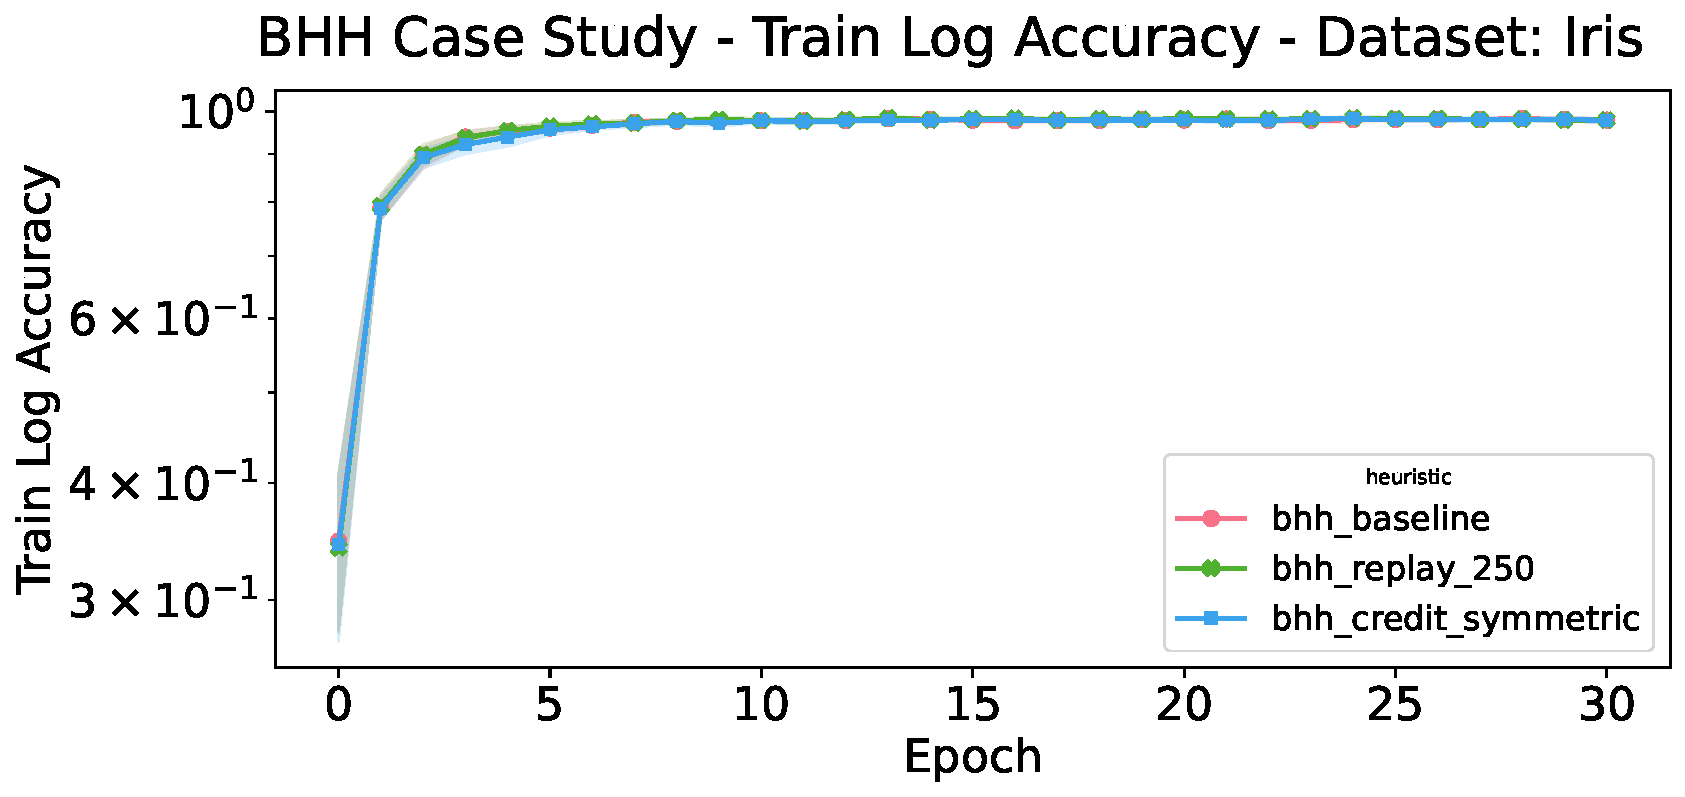
\includegraphics[width=1.0\textwidth]{case_study/metrics/figures/train/train_accuracy.pdf}
            \caption{Train log accuracy}
            \label{fig:results:case_study:metrics:train_accuracy}
      \end{subfigure}
      \begin{subfigure}{0.5\textwidth}
            \centering
            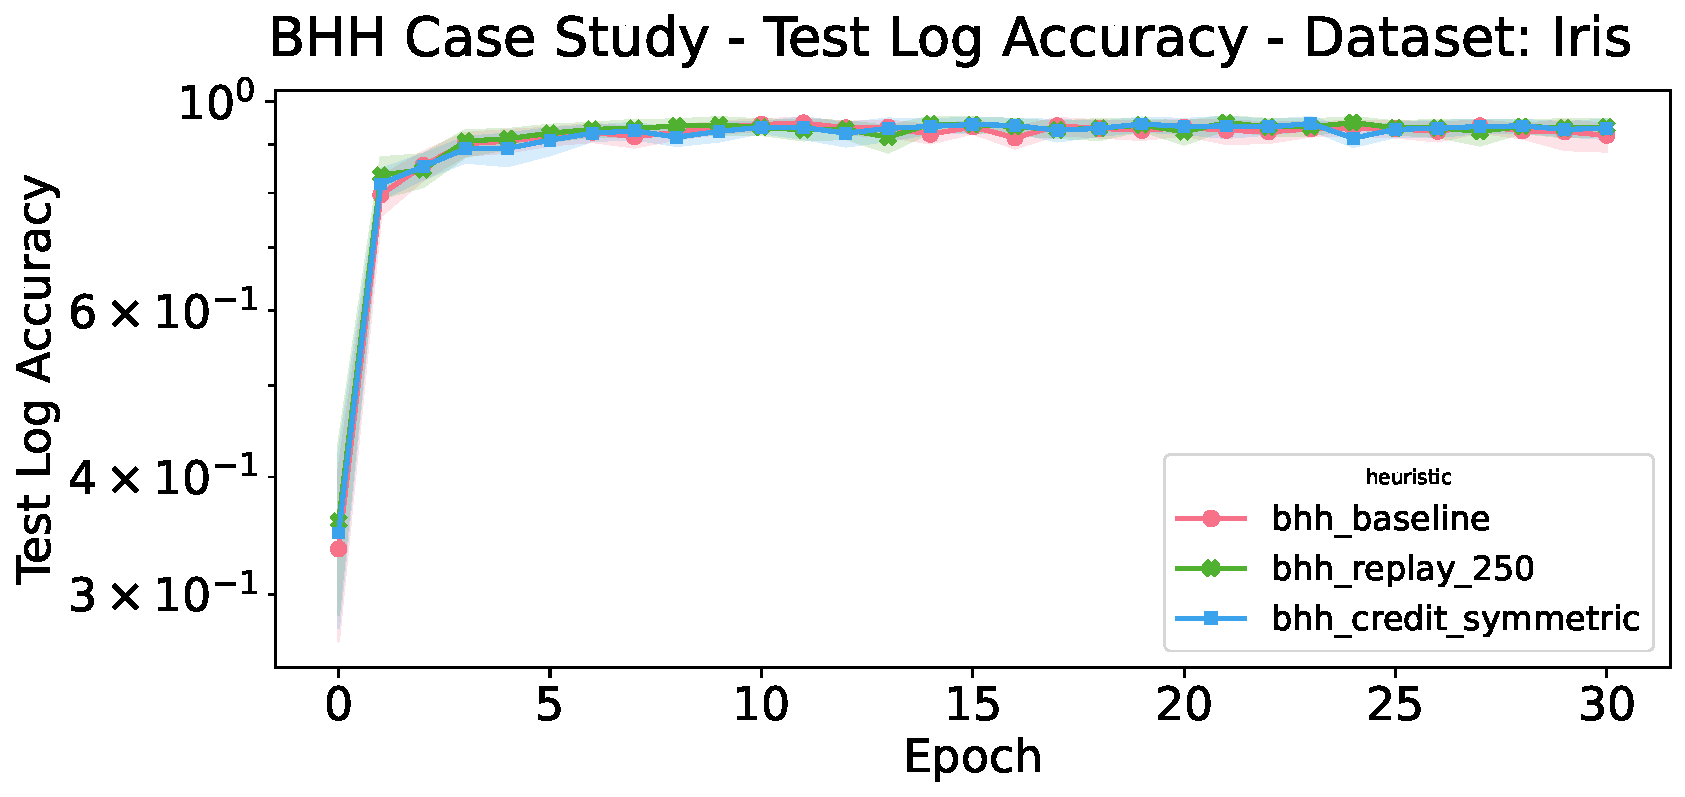
\includegraphics[width=1.0\textwidth]{case_study/metrics/figures/test/test_accuracy.pdf}
            \caption{Test log accuracy}
            \label{fig:results:case_study:metrics:test_accuracy}
      \end{subfigure}
      \par\bigskip
      \caption{The average train and test loss and accuracy plots over 30 epochs, obtained from 30 runs of the case study on the behaviour of the \acs{BHH} on the iris dataset, illustrated in log scale.}
      \label{fig:results:case_study:metrics}
\end{figure}

The first logical observation that can be made is that the \acs{BHH} was indeed able to successfully train the underlying \acs{FFNN}, observed by the convergence of the training process, yielding good results. Figures~\ref{fig:results:case_study:metrics:train_accuracy} and~\ref{fig:results:case_study:metrics:test_accuracy} show that the trained \acs{FFNN} achieved an accuracy of almost 100\%.

Although the different configurations of the \acs{BHH} are all able to succesfully train the underlying \acs{FFNN}, in this particular case, there is no clear distinction between the performance of any of the configurations under consideration.

The volatility and minor divergence of the test loss compared to the training loss, observed in Figure~\ref{fig:results:case_study:metrics:test_loss}, is due to overfitting and partly due to the noisiness that results from mini-batch training. Early stopping can be applied to the training process to halt training before the model overfits on the training data. The training dataset is also very small, with just 120 samples. Furthermore, a very small batch size of 16 is used. As such, noisiness and overfitting can be expected.

From Figure~\ref{fig:results:case_study:metrics:train_loss}, at the 22nd epoch, a small divergence of the train loss can be observed. This could simply be a result of momentum that is maintained when switching between low-level \index{heuristic}heuristics in an attempt to find better solutions. For example, momentum can be built up by one of the gradient-based heuristics, after which the \acs{BHH} switches to another heuristic in an attempt to find better solutions. The \acs{BHH} does not incorporate a \textit{move-acceptance strategy}, whereby a heuristic's outcome is rejected if it does not improve on previous solutions, yielding a possibly worse loss measurement as it relates to the test set. A move-acceptance strategy can be utilised on a validation set as a mechanism to accept or reject heuristic progressions from one step to the other.

Finally, it should be noted that the \acs{BHH} implements learning at every mini-batch step, while Figure~\ref{fig:results:case_study:metrics} only provides the outcomes of performance metrics at the end of each epoch. Further investigation is required at a mini-batch step level and is provided in the following sections.


% %%%%%%%%%%%%%%%%%%%%%%%%%%%%%%%%%%%%%%%%%%%%%%%%%%%%%
% % PARAMS ALPHAS
% %%%%%%%%%%%%%%%%%%%%%%%%%%%%%%%%%%%%%%%%%%%%%%%%%%%%%

\subsection{Concentration Parameters}\label{sec:results:case_study:concentration_parameters}

To illustrate the learning process undergone by the \acs{BHH}, further investigation is required. Consider the concentration parameter $\boldsymbol{\alpha}$ that parameterises the \index{Dirichelet probability distribution}Dirichelet probability distribution, denoted $P(\boldsymbol{\theta} \vert \boldsymbol{\alpha})$. The probability distribution, $P(\boldsymbol{\theta} \vert \boldsymbol{\alpha})$, is used to sample prior \textit{\index{heuristic}heuristic selection probabilities}. Figures~\ref{fig:results:case_study:alphas:0} to \ref{fig:results:case_study:alphas:8} provide illustrations that show that change in values of the concentration parameter $\boldsymbol{\alpha}$, at indices 0, 6, 7, and 8 respectively. Indices 0, 6, 7, and 8 represent the concentration parameters for the \acs{SGD}, \acs{Adam}, \acs{PSO} and \acs{GA} low-level heuristics respectively, and only represent a subset of the elements in $\boldsymbol{\alpha}$ and thus, the \index{heuristic pool}heuristic pool. Similar illustrations for the other elements in $\boldsymbol{\alpha}$ are left out for brevity as they contain similar illustrations.

\begin{figure}[htb]
      \begin{subfigure}{0.5\textwidth}
            \centering
            \includegraphics[width=1.0\textwidth]{case_study/params/figures/alphas/alpha[0].pdf}
            \caption{$\alpha_{0}$ - \acs{SGD}}
            \label{fig:results:case_study:alphas:0}
      \end{subfigure}
      \begin{subfigure}{0.5\textwidth}
            \centering
            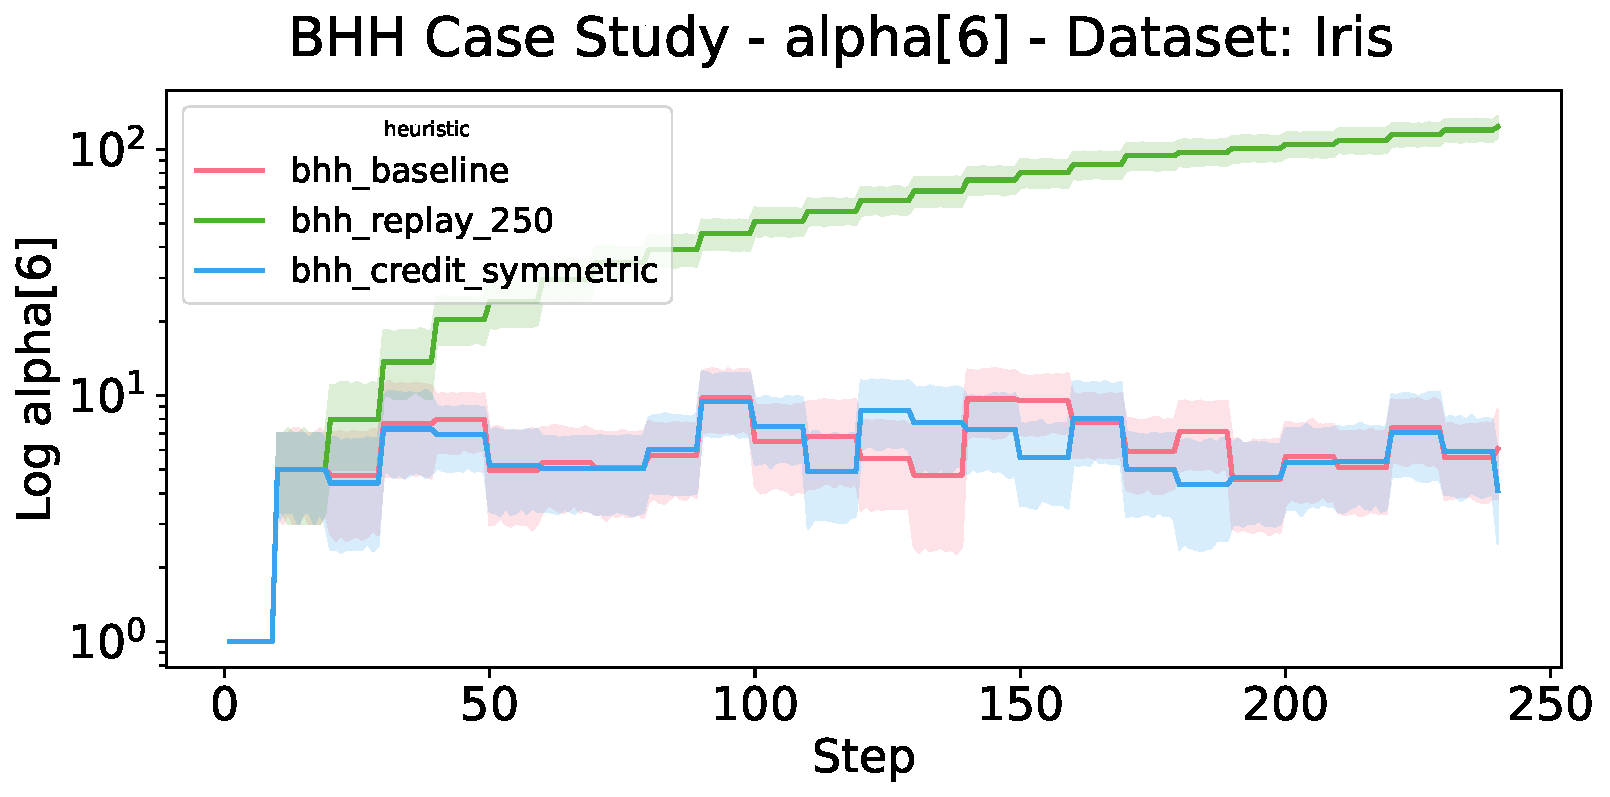
\includegraphics[width=1.0\textwidth]{case_study/params/figures/alphas/alpha[6].pdf}
            \caption{$\alpha_{6}$ - \acs{Adam}}
            \label{fig:results:case_study:alphas:6}
      \end{subfigure}
      \par\bigskip
      \begin{subfigure}{0.5\textwidth}
            \centering
            \includegraphics[width=1.0\textwidth]{case_study/params/figures/alphas/alpha[7].pdf}
            \caption{$\alpha_{7}$ - \acs{PSO}}
            \label{fig:results:case_study:alphas:7}
      \end{subfigure}
      \begin{subfigure}{0.5\textwidth}
            \centering
            \includegraphics[width=1.0\textwidth]{case_study/params/figures/alphas/alpha[8].pdf}
            \caption{$\alpha_{8}$ - \acs{GA}}
            \label{fig:results:case_study:alphas:8}
      \end{subfigure}
      \par\bigskip
      \caption{The average value of the concentration parameter $\boldsymbol{\alpha}$, at indices 0, 6, 7, and 8 over 240 steps, obtained from 30 runs of the case study on the behaviour of the \acs{BHH} on the iris dataset, illustrated in log scale.}
      \label{fig:results:case_study:alphas}
\end{figure}

The first logical observation to be made from Figures~\ref{fig:results:case_study:alphas:0} to \ref{fig:results:case_study:alphas:8} is the step-wise, increasing nature of $\boldsymbol{\alpha}$ for the bhh\_replay\_250 configuration, illustrated in \textcolor{green}{green}. Since the replay window size is sufficienty large to contain the performance log for all the steps executed in the training process, the \acs{BHH} does not forget past performances of low-level heuristics at all. The value for $\boldsymbol{\alpha}$ is never reset to its initial value of 1.0, and thus, $\boldsymbol{\alpha}$ continues to increase throughout the training process. However, it should be noted that the rate and degree of change is different for different indices of $\boldsymbol{\alpha}$. The aforementioned observation is the first indicator of the learning process yielded by the \acs{BHH}. Heuristics that perform well will see their corresponding element in $\boldsymbol{\alpha}$ increase more rapidly than other heuristics that do not perform well.

The next observations that can be made are for the bhh\_baseline configuration, illustrated in \textcolor{red}{red}, and the bhh\_credit\_symmetric configuration in \textcolor{blue}{blue}. Both these configurations see $\boldsymbol{\alpha}$ being reset to its initial value of 1.0 as regular intervals. This interval is defined by the \textit{reanalysis interval} hyper-parameter. The reanalysis interval dictates the frequency at which Bayesian analysis is conducted on the performance log, mainted by the \acs{BHH}. Bayesian analysis is used to update $\boldsymbol{\alpha}$ only at the reanalysis interval. As a result, small plateaus appear where $\boldsymbol{\alpha}$ does not change.

Notice from Figure~\ref{fig:results:case_study:alphas} that $\boldsymbol{\alpha} \geq 1.0$ for multiple elements. This is due to the accumulation of pseudo counts for $\boldsymbol{\alpha}$ by the Bayesian analysis process. Furthermore, this is also because the same heuristic can be allocated to multiple entities, each contributing a minimum pseudo-count gain of 1.0 to the corresponding element in $\boldsymbol{\alpha}$ through the Bayesian analysis process. Consider a case where all five entities in the entity pool are allocated the same heuristic and that a the replay window size of 10 is used. Then for all ten samples defined in the performance log, $\alpha_{i} = 50$, where $i$ is the index of the $i$-th \index{heuristic}heuristic in the \index{heuristic pool}heuristic pool.

Furthermore, it is important to mention that a change in $\boldsymbol{\alpha}$ between reanalysis windows does not yet necessarily indicate that the \acs{BHH} is learning. The concentration parameter $\boldsymbol{\alpha}$ tracks the \textit{occurrence} of the random event of observing heuristics (denoted $\boldsymbol{{H}}$). \index{heuristic}Heuristics can be observed as a result of good performance, by which the \acs{BHH} then learns to frequenctly reselect these \index{heuristic}heuristics again, or just by chance through the stochastic nature of probabilistic sampling as implemented by the \acs{BHH}. Further investigation is required to illustrate the learning mechanism of the \acs{BHH}.


% %%%%%%%%%%%%%%%%%%%%%%%%%%%%%%%%%%%%%%%%%%%%%%%%%%%%%
% % PARAMS THETAS
% %%%%%%%%%%%%%%%%%%%%%%%%%%%%%%%%%%%%%%%%%%%%%%%%%%%%%

\subsection{Probability Distribution of Heuristic Selection Probabilities}\label{sec:results:case_study:probs_of_select_probs}

This section provides a detailed investigation into the \textit{probability distribution of \index{heuristic}heuristic selection probabilities} as it changes throughout the training process. As a reminder, the \acs{BHH} implements a Bayesian view of probabilistic modeling and thus, \index{heuristic}heuristic selection probabilities are defined by an underlying probablistic distribution themselves. The probability distribution of \index{heuristic}heuristic selection probabilities is denoted by $P(\boldsymbol{\theta} \vert \boldsymbol{\alpha})$, where $\boldsymbol{\theta} \sim Dir(\boldsymbol{\alpha, K})$ are the sampled heuristic selection probabilities.

Figures~\ref{fig:results:case_study:thetas:0} to \ref{fig:results:case_study:thetas:8} provide illustrations of the distribution of \index{heuristic}heuristic selection probabilities, $\boldsymbol{\theta}$, sampled from the probability distribution $P(\boldsymbol{\theta} \vert \boldsymbol{\alpha})$ throughout the training process, and averaged over all 30 runs. These illustrations are presented in log scale. Indices 0, 6, 7, and 8 represent the distribution of \index{heuristic}heuristic selection probabilities for the \acs{SGD}, \acs{Adam}, \acs{PSO} and \acs{GA} low-level heuristics respectively, and only represent a subset of the distribution of \index{heuristic}heuristic selection probabilities in $\boldsymbol{\theta}$. Similar illustrations for the other elements in $\boldsymbol{\theta}$ are left out for brevity as they contain similar illustrations.

\begin{figure}[htb]
      \begin{subfigure}{0.5\textwidth}
            \centering
            \includegraphics[width=1.0\textwidth]{case_study/params/figures/thetas/theta[0].pdf}
            \caption{P($\theta_{0} \vert \alpha_{0})$ - \acs{SGD}}
            \label{fig:results:case_study:thetas:0}
      \end{subfigure}
      \begin{subfigure}{0.5\textwidth}
            \centering
            \includegraphics[width=1.0\textwidth]{case_study/params/figures/thetas/theta[6].pdf}
            \caption{P($\theta_{6} \vert \alpha_{6})$ - \acs{Adam}}
            \label{fig:results:case_study:thetas:6}
      \end{subfigure}
      \par\bigskip
      \begin{subfigure}{0.5\textwidth}
            \centering
            \includegraphics[width=1.0\textwidth]{case_study/params/figures/thetas/theta[7].pdf}
            \caption{P($\theta_{7} \vert \alpha_{7})$ - \acs{PSO}}
            \label{fig:results:case_study:thetas:7}
      \end{subfigure}
      \begin{subfigure}{0.5\textwidth}
            \centering
            \includegraphics[width=1.0\textwidth]{case_study/params/figures/thetas/theta[8].pdf}
            \caption{P($\theta_{8} \vert \alpha_{8})$ - \acs{GA}}
            \label{fig:results:case_study:thetas:8}
      \end{subfigure}
      \par\bigskip
      \caption{The average sampled \index{heuristic}heuristic selection probabilities, denoted $\boldsymbol{\theta}$, at indices 0, 6, 7, and 8. The \index{heuristic}heuristic selection probabilities are sampled from the probability distribution, denoted $P(\boldsymbol{\theta} \vert \boldsymbol{\alpha})$, over 240 steps, obtained from 30 runs of the case study on the behaviour of the \acs{BHH} on the iris dataset, illustrated in log scale.}
      \label{fig:results:case_study:thetas}
\end{figure}


From the illustrations presented in Figures~\ref{fig:results:case_study:thetas:0} to \ref{fig:results:case_study:thetas:8}, a clearer picture of the learning process of the \acs{BHH} is formed. The first important observation to make is for the bhh\_replay\_250 configuration, presented in \textcolor{green}{green}. As a reminder, ten low-level \index{heuristic}heuristics are included in the heuristic pool, yielding an expected mean \index{heuristic}heuristics selection probability of 0.1, for each \index{heuristic}heuristic, by the frequentist view of probabilistic modeling.

Towards the end of the training process, the \index{heuristic}heuristic selection probability converges back to the symmetrical, uniform probability distribution, yielding a \index{heuristic}heuristic selection probability of 0.1, for all \index{heuristic}heuristics. This can be explained as follows: most of the training progress is made in the early stages of the training process, and training converges towards the end of the training process. Since training converges, all heuristics, no matter their past performances, fail to yield better solutions towards the end of the training process. As a result of training convergence, heuristics then fail to meet the performance criteria and credit allocations by means of the credit assignment strategy.

Both the bhh\_baseline (\textcolor{red}{red}) and the bhh\_replay\_250 (\textcolor{green}{green}) configurations make use of the \textit{ibest} credit assignment strategy. The \textit{ibest} credit assignment strategy allocates credit to the heuristic that yields the best performance for the current iteration/step and thus, towards the end of the training process, any random heuristic can yield the best iteration performance. However, since the bhh\_baseline is configured with a small replay window size of 10, and a reanalysis interval of 10, the concentration parameter $\boldsymbol{\alpha}$ is reset to its default value of 1.0 more often than the bhh\_replay\_250 configuration, resulting in a probability distribution that is broader, and thus, explaining the larger variance of $\boldsymbol{\theta}$ throughout.

Another observation to make occurs in the first 30 steps of the training process. In Figure~\ref{fig:results:case_study:thetas}, notice how all three configurations mostly yield the same \index{heuristic}heuristic selection probabilities in these first 30 steps. This can be explained as follows: all three configurations use a different random seed per run, but use the same random seed across configurations for the same run number. This is done so that any difference in the behaviour of the different \acs{BHH} configurations are then not a result of random sampling, but solely because of differences in their approaches. This is especially applicable to the initialisation process, where entities are randomly placed in the search space, as well as the early stages of training, where most of the training progress is made.

It should be noted that, despite using the same random seed across configurations for the same run number, the behavioural changes between the configurations start to show after about 30 steps. As a reminder, the bhh\_credit\_symmetric (\textcolor{blue}{blue}) configuration, does not bias towards best performing \index{heuristic}heuristics. Where the bhh\_baseline and bhh\_replay\_250 configurations then diverge from the behaviour of the bhh\_credit\_symmetric configuration is proof of the effect of performance bias.

Furthermore, it can be observed for small windows, at various steps for multiple runs, that the variance of $\boldsymbol{\theta}$, for the bhh\_baseline configuration and the bhh\_credit\_symmetric configuration, do not yield means that are equal to the expected \index{heuristic}heuristic selection probabilities of 0.1. This is proof that the \acs{BHH} does not just implement a form of random search, despite having small reanalysis interval and replay window size configurations. This is also true for the bhh\_credit\_symmetric configuration, as the bhh\_credit\_symmetric configuration biases towards heuristics that happen to be sampled, despite not biasing towards good performance.

Finally, the bhh\_baseline configuration and the bhh\_credit\_symmetric configuration both yield similar volatile behaviour, much more so than with the bhh\_replay\_250 configuration. This can be attributed to a very small reanalysis window combined with a small replay window size of 10, that contains very few samples to learn from. A small reanalysis interval and a small replay window size allows for more exploration of the \index{heuristic}heuristic space, but can also yield greater variance of the \index{heuristic}heuristic selection probabilities. Once again, any differences then in the behaviour of the bhh\_baseline compared to the bhh\_credit\_symmetric configurations is proof of small performance exploitations and biases by the bhh\_baseline configuration.


% %%%%%%%%%%%%%%%%%%%%%%%%%%%%%%%%%%%%%%%%%%%%%%%%%%%%%
% % PARAMS P_H (Priors)
% %%%%%%%%%%%%%%%%%%%%%%%%%%%%%%%%%%%%%%%%%%%%%%%%%%%%%

\subsection{Prior Heuristic Selection Probabilities}\label{sec:results:case_study:prior_selec_prob}

This section provides a brief investigation into the \textit{prior \index{heuristic}heuristic selection probabilities} that result from the probabilistic model implemented by the \acs{BHH}. The prior \index{heuristic}heuristic selection probability distribution is denoted $P(\boldsymbol{H} \vert \boldsymbol{\theta})$. As such, $P(\boldsymbol{H} \vert \boldsymbol{\theta}) = \boldsymbol{\theta}$ and heuristics are initially sampled such that $\boldsymbol{H} \sim Cat(\boldsymbol{\theta})$.

Figures~\ref{fig:results:case_study:p_H:0} to \ref{fig:results:case_study:p_H:8} provide illustrations of the prior \index{heuristic}heuristic selection probabilities, denoted by $P(\boldsymbol{H} \vert \boldsymbol{\theta})$, at indices 0, 6, 7, and 8, throughout the training process, and averaged over all 30 runs. Similar to before, these illustrations are also presented in log scale.

\begin{figure}[htb]
      \begin{subfigure}{0.5\textwidth}
            \centering
            \includegraphics[width=1.0\textwidth]{case_study/params/figures/p_H/p_H[0].pdf}
            \caption{P($h_{0} \vert \theta_{0})$ - \acs{SGD}}
            \label{fig:results:case_study:p_H:0}
      \end{subfigure}
      \begin{subfigure}{0.5\textwidth}
            \centering
            \includegraphics[width=1.0\textwidth]{case_study/params/figures/p_H/p_H[6].pdf}
            \caption{P($h_{6} \vert \theta_{6})$ - \acs{Adam}}
            \label{fig:results:case_study:p_H:6}
      \end{subfigure}
      \par\bigskip
      \begin{subfigure}{0.5\textwidth}
            \centering
            \includegraphics[width=1.0\textwidth]{case_study/params/figures/p_H/p_H[7].pdf}
            \caption{P($h_{7} \vert \theta_{7})$ - \acs{PSO}}
            \label{fig:results:case_study:p_H:7}
      \end{subfigure}
      \begin{subfigure}{0.5\textwidth}
            \centering
            \includegraphics[width=1.0\textwidth]{case_study/params/figures/p_H/p_H[8].pdf}
            \caption{P($h_{8} \vert \theta_{8})$ - \acs{GA}}
            \label{fig:results:case_study:p_H:8}
      \end{subfigure}
      \par\bigskip
      \caption{The average prior \index{heuristic}heuristic selection probabilities, $P(\boldsymbol{H} \vert \boldsymbol{\theta})$, at indices 0, 6, 7, and 8. The prior \index{heuristic}heuristic selection probabilities are sampled from the probability distribution of \index{heuristic}heuristic selection probabilities, denoted by $P(\boldsymbol{\theta} \vert \boldsymbol{\alpha})$, over 240 steps, obtained from 30 runs of the case study on the behaviour of the \acs{BHH} on the iris dataset, illustrated in log scale.}
      \label{fig:results:case_study:p_H}
\end{figure}

The main observation to make from these figures is that they are much less volatile and noisy than the figures presented for the distribution of \index{heuristic}heuristic selection probabilities, $\boldsymbol{\theta}$, presented in the previous section in Figure~\ref{fig:results:case_study:thetas}. This is because of the \textit{reselection} interval hyper-parameter. The reselection interval hyper-parameter is implemented as a way to control the frequency by which new heuristics are selected and allocated to each entity. Since the default \textit{reselection} interval is set to 10, the \index{heuristic}heuristic selection probabilities are only resampled at intervals of 10. These illustrations then simply yield rough approximations of the illustrations provided in Figures~\ref{fig:results:case_study:thetas:0} to \ref{fig:results:case_study:thetas:8} for the distribution of \index{heuristic}heuristic selection probabilities. As such, the same observations and conclusions that are made in Section \ref{sec:results:case_study:probs_of_select_probs} also apply in this section.

Finally, it should be mentioned that at each step, the goal of the \acs{BHH} is to update these prior ``beliefs'' based on newly observed evidence of \index{heuristic}heuristic performances. Since these prior \index{heuristic}heuristic selection probabilities change over time, it can be concluded that the change in prior \index{heuristic}heuristic selection probabilities is a result of the learning mechanism of the \acs{BHH}. Furthermore, the prior \index{heuristic}heuristic selection probability distribution provides an opportunity to utilise prior knowledge by some expert before training starts, by injecting heuristic selection biases, by means of the initial values for the concentration parameter $\boldsymbol{\alpha}$.



% %%%%%%%%%%%%%%%%%%%%%%%%%%%%%%%%%%%%%%%%%%%%%%%%%%%%%
% % PARAMS P_HgEC (Posterior)
% %%%%%%%%%%%%%%%%%%%%%%%%%%%%%%%%%%%%%%%%%%%%%%%%%%%%%

\subsection{Posterior Heuristic Selection Probabilities}\label{sec:results:case_study:posterior_selec_prob}

This section provides a detailed discussion on the outcomes of the \textit{posterior heuristic selection probabilities}. These posterior heuristic selection probabilities form the basis of the probabilistic model implemented by the \acs{BHH}. The posterior \index{heuristic}heuristic selection probability distribution is defined as $P(\boldsymbol{H} \vert \boldsymbol{E}, \boldsymbol{C}; \boldsymbol{\theta}, \boldsymbol{\phi}, \boldsymbol{\psi})$, where $\boldsymbol{E}$ represents the vector of entities in the entity pool, and $\boldsymbol{C}$ represents the vector of credit allocation outcomes as implemented by the credit assignment strategy. Furthermore $\boldsymbol{\theta}$ and $\boldsymbol{\phi}$ represent the probability distributions of \index{heuristic}heuristic selection probabilities and the entity selection probabilities respectively. Finally, $\boldsymbol{\psi}$ represents the probability distribution of successful credit allocation probabilities.

Figures~\ref{fig:results:case_study:p_HgEC:0:0} to \ref{fig:results:case_study:p_HgEC:0:8} provide illustrations of the calculated posterior \index{heuristic}heuristic selection probabilities at indices 0, 6, 7, and 8, throughout the training process, averaged over 30 runs. Similar to before, these illustrations are also presented in log scale. As before, illustrations for the other indices are left out for brevity as they yield simular illustrations.

\begin{figure}[htb]
      \begin{subfigure}{0.5\textwidth}
            \centering
            \includegraphics[width=1.0\textwidth]{case_study/params/figures/p_HgEC/p_HgEC[0][0].pdf}
            \caption{$P(h_{0} \vert e_{0}, c_{1})$ - \acs{SGD}}
            \label{fig:results:case_study:p_HgEC:0:0}
      \end{subfigure}
      \begin{subfigure}{0.5\textwidth}
            \centering
            \includegraphics[width=1.0\textwidth]{case_study/params/figures/p_HgEC/p_HgEC[0][6].pdf}
            \caption{$P(h_{6} \vert e_{0}, c_{1})$ - \acs{Adam}}
            \label{fig:results:case_study:p_HgEC:0:6}
      \end{subfigure}
      \par\bigskip
      \begin{subfigure}{0.5\textwidth}
            \centering
            \includegraphics[width=1.0\textwidth]{case_study/params/figures/p_HgEC/p_HgEC[0][7].pdf}
            \caption{$P(h_{7} \vert e_{0}, c_{1})$ - \acs{PSO}}
            \label{fig:results:case_study:p_HgEC:0:7}
      \end{subfigure}
      \begin{subfigure}{0.5\textwidth}
            \centering
            \includegraphics[width=1.0\textwidth]{case_study/params/figures/p_HgEC/p_HgEC[0][8].pdf}
            \caption{$P(h_{8} \vert e_{0}, c_{1})$ - \acs{GA}}
            \label{fig:results:case_study:p_HgEC:0:8}
      \end{subfigure}
      \par\bigskip
      \caption{The average calculated proportional posterior \index{heuristic}heuristic selection probabilities for \index{heuristic}heuristics $(\boldsymbol{H})$ at indices 0, 6, 7, and 8, given the application to entity $e_{0}$ and requiring a successful credit allocation, $c_{1}$, from the \textit{ibest} credit assignment strategy. The proportional posterior \index{heuristic}heuristic selection probabilities are calculated from the probabilistic model, denoted $P(\boldsymbol{H} \vert \boldsymbol{E}, \boldsymbol{C}; \boldsymbol{\theta}, \boldsymbol{\phi}, \boldsymbol{\psi})$, over 240 steps, and obtained from 30 runs of the case study on the behaviour of the \acs{BHH} on the iris dataset, illustrated in log scale.}
      \label{fig:results:case_study:p_HgEC:0}
\end{figure}

The main observation to make from Figures~\ref{fig:results:case_study:p_HgEC:0:0} to \ref{fig:results:case_study:p_HgEC:0:8} is that the implemented posterior heuristic selection distribution, defined by $P(\boldsymbol{H} \vert \boldsymbol{E}, \boldsymbol{C}; \boldsymbol{\theta}, \boldsymbol{\phi}, \boldsymbol{\psi})$, does not yield normalised probabilities, but rather yield unnormalised \textit{logits}, which are used to parameterise a \index{Categorical probability distribution}Categorical probability distribution from which new \index{heuristic}heuristic selections are sampled. The reasons for the aforementioned is because the probablistic model is evaluated proportionaly as was discussed in Chapter~\ref{chap:bhh}. As a reminder, the log-sum-exp trick is used in order to maintain numerical stability, yielding \textit{logits} instead of probabilities.

Another observation to make is for the bhh\_replay\_250 configuration $(\textcolor{green}{green})$. Figures~\ref{fig:results:case_study:p_HgEC:0:0} to \ref{fig:results:case_study:p_HgEC:0:8} show that the posterior heuristic selection probabilities converge to the expected heuristic selection probabilities later in the training stages. The aforementioned suggests that the \acs{BHH} is not able to find anymore performance biases and cannot exploit better solutions. At this point, the \acs{BHH} starts to explore more as the concentration parameters are reanalysed more uniformly, resolving more and more to a random search in attempt to find better solutions.

Furthermore, the posterior heuristic selection probability distribution is conditional on the occurrence of a specific entity that the potential \index{heuristic}heuristic will be applied to, as well as a specific performance criterion enforced by a specific credit assignment strategy. This means that \index{heuristic}heuristic selection is specific to each entity. A particular \index{heuristic}heuristic might be good for one entity, but not for another. This is a strong characteristic of the \acs{BHH}, as it learns to apply the correct \index{heuristic}heuristic to the correct entity at the correct time in the training process.

Finally, the posterior heuristic selection probabilities are much less volatile than their prior heuristic selection probability equivalents. This is a result of the information that is added in the performance log by tracking the entity and credit allocation as well.

It can be concluded from Sections~\ref{sec:results:case_study:performance_metrics} to \ref{sec:results:case_study:posterior_selec_prob} that the \acs{BHH} is able to successfully train the underlying \acs{FFNN} for the case study on the iris dataset. Furthermore it can be concluded that the learning mechanism implemented by the \acs{BHH} is able to exploit minor performance biases, and thus the \acs{BHH} is able to correctly allocate the correct heuristic to the correct entity at the correct time in the training process.

%%%%%%%%%%%%%%%%%%%%%%%%%%%%%%%%%%%%%%%%%%%%%%%%%%%%%%%%%%%%%%%5
% BHH vs. Low-Level Heuristics
%%%%%%%%%%%%%%%%%%%%%%%%%%%%%%%%%%%%%%%%%%%%%%%%%%%%%%%%%%%%%%%5
\section{BHH vs. Low-Level Heuristics}\label{sec:results:standalone}

This section provides the empirical results for the experimental group that compares the performance of the \acs{BHH} to the performance of the individual, standalone, low-level heuristics. Detailed discussions and illustrations follow. As a reminder, the set of low-level heuristics includes a number of gradient-based heuristics and a number of \acp{MH}. Three variants of the \acs{BHH} is included in the experiment, including the \acs{BHH} baseline configuration with a \index{heuristic pool}heuristic pool that contains all the low-level heuristics (denoted bhh\_all), the \acs{BHH} configuration with a \index{heuristic pool}heuristic pool that contains only gradient-based \index{heuristic}heuristics (denoted bhh\_gd), and finally, the \acs{BHH} configuration with a \index{heuristic pool}heuristics pool that contains only \index{meta-heuristic}meta-heuristics (denoted bhh\_mh).

Table~\ref{tab:results:standalone:metrics:loss} presents the empirical results for this experimental group, showing the average test loss and statistics for all the low-level heuristics, compared to the three variants of the \acs{BHH} that was implemented. The test loss is measured at the last epoch for each dataset, over all independent runs.

\begin{sidewaystable}[htbp]
      \centering
      \caption{Empirical results showing test loss and statistics for different low-level \index{heuristic}heuristics compared to three \index{heuristic pool}heuristic pool variants of the \acs{BHH} baseline configuration, across multiple datasets, for all independent runs, measured at the last epoch.}
      \label{tab:results:standalone:metrics:loss}%
      \par\bigskip
      \resizebox{\textwidth}{!}{
            \begin{tabular}{r|lll|l|l|l|l|l|lllll}
                                                      & \multicolumn{13}{c}{\textbf{BHH vs. Low-Level Heuristics - Average Test Loss}}                                                                                                                                                                                                                                                                                                                                                                                                                                                                                                                                                                                                                                                                                                                         \\
                  \cmidrule{2-14}    \textbf{dataset} & \multicolumn{1}{c}{\textbf{adagrad}}                                           & \multicolumn{1}{c}{\textbf{adam}}                       & \multicolumn{1}{c|}{\textbf{rmsprop}}                   & \multicolumn{1}{c|}{\textbf{bhh\_gd}}                   & \multicolumn{1}{c|}{\textbf{nag}}                       & \multicolumn{1}{c|}{\textbf{bhh\_all}}                  & \multicolumn{1}{c|}{\textbf{adadelta}}                  & \multicolumn{1}{c|}{\textbf{bhh\_mh}}                   & \multicolumn{1}{c}{\textbf{ga}}                         & \multicolumn{1}{c}{\textbf{pso}}                        & \multicolumn{1}{c}{\textbf{sgd}}                        & \multicolumn{1}{c}{\textbf{momentum}}                   & \multicolumn{1}{c}{\textbf{de}}                         \\
                  \midrule
                  \textbf{abalone}                    & \cellcolor[rgb]{ .506,  .776,  .486}1.9678 ($\pm$0.032)                        & \cellcolor[rgb]{ .494,  .773,  .486}1.9651 ($\pm$0.035) & \cellcolor[rgb]{ .388,  .745,  .482}1.9455 ($\pm$0.035) & \cellcolor[rgb]{ .749,  .847,  .502}2.0125 ($\pm$0.068) & \cellcolor[rgb]{ .765,  .851,  .502}2.0156 ($\pm$0.035) & \cellcolor[rgb]{ 1,  .922,  .518}2.0587 ($\pm$0.088)    & \cellcolor[rgb]{ .788,  .859,  .502}2.0199 ($\pm$0.034) & \cellcolor[rgb]{ .996,  .827,  .502}2.2942 ($\pm$0.055) & \cellcolor[rgb]{ .984,  .612,  .459}2.8155 ($\pm$0.055) & \cellcolor[rgb]{ .98,  .522,  .443}3.0384 ($\pm$0.294)  & \cellcolor[rgb]{ .992,  .773,  .49}2.428 ($\pm$0.029)   & \cellcolor[rgb]{ .992,  .745,  .486}2.4942 ($\pm$0.029) & \cellcolor[rgb]{ .973,  .412,  .42}3.2959 ($\pm$0.016)  \\
                  \textbf{air quality}                & \cellcolor[rgb]{ .651,  .82,  .494}0.2569 ($\pm$0.007)                         & \cellcolor[rgb]{ .827,  .871,  .506}0.2606 ($\pm$0.009) & \cellcolor[rgb]{ .388,  .745,  .482}0.2513 ($\pm$0.008) & \cellcolor[rgb]{ 1,  .922,  .518}0.2642 ($\pm$0.011)    & \cellcolor[rgb]{ .647,  .82,  .494}0.2568 ($\pm$0.006)  & \cellcolor[rgb]{ .996,  .827,  .502}0.2729 ($\pm$0.016) & \cellcolor[rgb]{ .647,  .82,  .494}0.2568 ($\pm$0.006)  & \cellcolor[rgb]{ .976,  .914,  .514}0.2637 ($\pm$0.007) & \cellcolor[rgb]{ .996,  .792,  .494}0.2759 ($\pm$0.008) & \cellcolor[rgb]{ .984,  .608,  .459}0.2923 ($\pm$0.023) & \cellcolor[rgb]{ .988,  .69,  .475}0.2852 ($\pm$0.015)  & \cellcolor[rgb]{ .984,  .604,  .459}0.2929 ($\pm$0.016) & \cellcolor[rgb]{ .973,  .412,  .42}0.3097 ($\pm$0.017)  \\
                  \textbf{bank}                       & \cellcolor[rgb]{ .459,  .765,  .486}0.2096 ($\pm$0.005)                        & \cellcolor[rgb]{ .4,  .745,  .482}0.2065 ($\pm$0.004)   & \cellcolor[rgb]{ .388,  .745,  .482}0.2058 ($\pm$0.006) & \cellcolor[rgb]{ .588,  .8,  .49}0.2164 ($\pm$0.005)    & \cellcolor[rgb]{ .588,  .8,  .49}0.2164 ($\pm$0.006)    & \cellcolor[rgb]{ 1,  .886,  .514}0.2456 ($\pm$0.065)    & \cellcolor[rgb]{ .627,  .812,  .494}0.2186 ($\pm$0.004) & \cellcolor[rgb]{ .996,  .839,  .502}0.2562 ($\pm$0.011) & \cellcolor[rgb]{ .988,  .686,  .475}0.2881 ($\pm$0.013) & \cellcolor[rgb]{ .973,  .412,  .42}0.3454 ($\pm$0.034)  & \cellcolor[rgb]{ 1,  .922,  .518}0.2382 ($\pm$0.006)    & \cellcolor[rgb]{ 1,  .922,  .518}0.2386 ($\pm$0.005)    & \cellcolor[rgb]{ .976,  .424,  .424}0.3437 ($\pm$0.028) \\
                  \textbf{bike}                       & \cellcolor[rgb]{ .388,  .745,  .482}0.0458 ($\pm$0.002)                        & \cellcolor[rgb]{ .592,  .804,  .494}0.0682 ($\pm$0.068) & \cellcolor[rgb]{ 1,  .922,  .518}0.1123 ($\pm$0.103)    & \cellcolor[rgb]{ .467,  .765,  .486}0.0545 ($\pm$0.005) & \cellcolor[rgb]{ .882,  .886,  .51}0.0995 ($\pm$0.002)  & \cellcolor[rgb]{ .565,  .796,  .49}0.0651 ($\pm$0.02)   & \cellcolor[rgb]{ .588,  .8,  .49}0.0679 ($\pm$0.002)    & \cellcolor[rgb]{ 1,  .902,  .514}0.1179 ($\pm$0.006)    & \cellcolor[rgb]{ .992,  .761,  .486}0.1531 ($\pm$0.005) & \cellcolor[rgb]{ .992,  .773,  .49}0.1503 ($\pm$0.025)  & \cellcolor[rgb]{ .992,  .733,  .482}0.1599 ($\pm$0.003) & \cellcolor[rgb]{ .992,  .725,  .482}0.1614 ($\pm$0.003) & \cellcolor[rgb]{ .973,  .412,  .42}0.2399 ($\pm$0.04)   \\
                  \textbf{car}                        & \cellcolor[rgb]{ .729,  .843,  .502}0.2027 ($\pm$0.018)                        & \cellcolor[rgb]{ .388,  .745,  .482}0.0972 ($\pm$0.024) & \cellcolor[rgb]{ .408,  .749,  .482}0.1039 ($\pm$0.031) & \cellcolor[rgb]{ .62,  .812,  .494}0.169 ($\pm$0.025)   & \cellcolor[rgb]{ .867,  .882,  .51}0.2454 ($\pm$0.029)  & \cellcolor[rgb]{ .58,  .8,  .49}0.1572 ($\pm$0.034)     & \cellcolor[rgb]{ 1,  .922,  .518}0.2859 ($\pm$0.027)    & \cellcolor[rgb]{ .992,  .733,  .482}0.4891 ($\pm$0.077) & \cellcolor[rgb]{ .98,  .502,  .439}0.7374 ($\pm$0.063)  & \cellcolor[rgb]{ .988,  .667,  .471}0.5632 ($\pm$0.158) & \cellcolor[rgb]{ .98,  .533,  .443}0.7035 ($\pm$0.052)  & \cellcolor[rgb]{ .98,  .506,  .439}0.7322 ($\pm$0.043)  & \cellcolor[rgb]{ .973,  .412,  .42}0.8332 ($\pm$0.074)  \\
                  \textbf{diabetic}                   & \cellcolor[rgb]{ .694,  .831,  .498}0.8895 ($\pm$0.004)                        & \cellcolor[rgb]{ 1,  .898,  .514}0.9193 ($\pm$0.01)     & \cellcolor[rgb]{ .918,  .894,  .51}0.8957 ($\pm$0.004)  & \cellcolor[rgb]{ .98,  .914,  .514}0.8976 ($\pm$0.011)  & \cellcolor[rgb]{ .388,  .745,  .482}0.8809 ($\pm$0.004) & \cellcolor[rgb]{ .973,  .412,  .42}1.2983 ($\pm$0.66)   & \cellcolor[rgb]{ .49,  .773,  .486}0.8839 ($\pm$0.005)  & \cellcolor[rgb]{ 1,  .902,  .518}0.9137 ($\pm$0.008)    & \cellcolor[rgb]{ .996,  .843,  .506}0.9613 ($\pm$0.007) & \cellcolor[rgb]{ .996,  .835,  .502}0.9661 ($\pm$0.016) & \cellcolor[rgb]{ .976,  .914,  .514}0.8974 ($\pm$0.004) & \cellcolor[rgb]{ 1,  .922,  .518}0.898 ($\pm$0.003)     & \cellcolor[rgb]{ .988,  .694,  .475}1.0774 ($\pm$0.039) \\
                  \textbf{fish toxicity}              & \cellcolor[rgb]{ .588,  .8,  .49}0.0991 ($\pm$0.008)                           & \cellcolor[rgb]{ .451,  .761,  .482}0.0972 ($\pm$0.007) & \cellcolor[rgb]{ .388,  .745,  .482}0.0963 ($\pm$0.008) & \cellcolor[rgb]{ 1,  .91,  .518}0.1056 ($\pm$0.008)     & \cellcolor[rgb]{ .831,  .871,  .506}0.1023 ($\pm$0.008) & \cellcolor[rgb]{ 1,  .922,  .518}0.1046 ($\pm$0.008)    & \cellcolor[rgb]{ .773,  .855,  .502}0.1016 ($\pm$0.009) & \cellcolor[rgb]{ .976,  .914,  .514}0.1043 ($\pm$0.009) & \cellcolor[rgb]{ 1,  .863,  .506}0.1093 ($\pm$0.009)    & \cellcolor[rgb]{ 1,  .855,  .506}0.1099 ($\pm$0.012)    & \cellcolor[rgb]{ .976,  .475,  .435}0.1393 ($\pm$0.012) & \cellcolor[rgb]{ .973,  .412,  .42}0.1441 ($\pm$0.012)  & \cellcolor[rgb]{ .992,  .733,  .482}0.1193 ($\pm$0.013) \\
                  \textbf{forest fires}               & \cellcolor[rgb]{ 1,  .922,  .518}0.0643 ($\pm$0.04)                            & \cellcolor[rgb]{ .557,  .792,  .49}0.0527 ($\pm$0.039)  & \cellcolor[rgb]{ 1,  .922,  .518}0.0626 ($\pm$0.039)    & \cellcolor[rgb]{ .824,  .871,  .506}0.0586 ($\pm$0.034) & \cellcolor[rgb]{ .851,  .878,  .506}0.0592 ($\pm$0.032) & \cellcolor[rgb]{ 1,  .89,  .514}0.081 ($\pm$0.069)      & \cellcolor[rgb]{ .388,  .745,  .482}0.0488 ($\pm$0.032) & \cellcolor[rgb]{ .976,  .914,  .514}0.0621 ($\pm$0.038) & \cellcolor[rgb]{ .553,  .792,  .49}0.0526 ($\pm$0.026)  & \cellcolor[rgb]{ 1,  .914,  .518}0.0692 ($\pm$0.047)    & \cellcolor[rgb]{ .992,  .722,  .482}0.1806 ($\pm$0.008) & \cellcolor[rgb]{ .992,  .706,  .478}0.1885 ($\pm$0.01)  & \cellcolor[rgb]{ .973,  .412,  .42}0.3598 ($\pm$0.09)   \\
                  \textbf{housing}                    & \cellcolor[rgb]{ .518,  .78,  .486}0.0889 ($\pm$0.012)                         & \cellcolor[rgb]{ .404,  .749,  .482}0.0848 ($\pm$0.011) & \cellcolor[rgb]{ .388,  .745,  .482}0.0842 ($\pm$0.015) & \cellcolor[rgb]{ .69,  .831,  .498}0.0951 ($\pm$0.015)  & \cellcolor[rgb]{ .612,  .808,  .494}0.0923 ($\pm$0.016) & \cellcolor[rgb]{ .663,  .824,  .498}0.0941 ($\pm$0.017) & \cellcolor[rgb]{ 1,  .922,  .518}0.106 ($\pm$0.019)     & \cellcolor[rgb]{ 1,  .867,  .51}0.1169 ($\pm$0.019)     & \cellcolor[rgb]{ .996,  .812,  .498}0.1279 ($\pm$0.02)  & \cellcolor[rgb]{ .992,  .722,  .482}0.1452 ($\pm$0.03)  & \cellcolor[rgb]{ .984,  .576,  .455}0.1735 ($\pm$0.023) & \cellcolor[rgb]{ .984,  .588,  .455}0.1713 ($\pm$0.018) & \cellcolor[rgb]{ .973,  .412,  .42}0.2057 ($\pm$0.036)  \\
                  \textbf{iris}                       & \cellcolor[rgb]{ .788,  .859,  .502}0.2161 ($\pm$0.059)                        & \cellcolor[rgb]{ .514,  .78,  .486}0.1203 ($\pm$0.098)  & \cellcolor[rgb]{ .388,  .745,  .482}0.0753 ($\pm$0.046) & \cellcolor[rgb]{ 1,  .855,  .506}0.3729 ($\pm$1.119)    & \cellcolor[rgb]{ .416,  .753,  .482}0.085 ($\pm$0.042)  & \cellcolor[rgb]{ .859,  .878,  .506}0.2411 ($\pm$0.295) & \cellcolor[rgb]{ .996,  .808,  .498}0.426 ($\pm$0.072)  & \cellcolor[rgb]{ .686,  .831,  .498}0.1809 ($\pm$0.164) & \cellcolor[rgb]{ 1,  .922,  .518}0.2895 ($\pm$0.117)    & \cellcolor[rgb]{ .973,  .412,  .42}0.8965 ($\pm$0.844)  & \cellcolor[rgb]{ .992,  .773,  .49}0.4694 ($\pm$0.088)  & \cellcolor[rgb]{ .992,  .745,  .486}0.5028 ($\pm$0.072) & \cellcolor[rgb]{ .98,  .494,  .435}0.8027 ($\pm$0.684)  \\
                  \textbf{mushroom}                   & \cellcolor[rgb]{ .549,  .792,  .49}0.0026 ($\pm$0.001)                         & \cellcolor[rgb]{ .467,  .765,  .486}0.0013 ($\pm$0.005) & \cellcolor[rgb]{ .388,  .745,  .482}0.0001 ($\pm$0)     & \cellcolor[rgb]{ .439,  .757,  .482}0.0009 ($\pm$0.001) & \cellcolor[rgb]{ 1,  .922,  .518}0.0094 ($\pm$0.002)    & \cellcolor[rgb]{ .718,  .839,  .498}0.0052 ($\pm$0.012) & \cellcolor[rgb]{ .655,  .82,  .494}0.0042 ($\pm$0.001)  & \cellcolor[rgb]{ 1,  .871,  .51}0.0774 ($\pm$0.02)      & \cellcolor[rgb]{ .984,  .561,  .451}0.4892 ($\pm$0.025) & \cellcolor[rgb]{ 1,  .886,  .514}0.0611 ($\pm$0.06)     & \cellcolor[rgb]{ .996,  .796,  .494}0.1797 ($\pm$0.009) & \cellcolor[rgb]{ .992,  .749,  .486}0.2418 ($\pm$0.013) & \cellcolor[rgb]{ .973,  .412,  .42}0.687 ($\pm$0.016)   \\
                  \textbf{parkinsons}                 & \cellcolor[rgb]{ .51,  .776,  .486}0.0563 ($\pm$0.001)                         & \cellcolor[rgb]{ .412,  .749,  .482}0.0545 ($\pm$0.002) & \cellcolor[rgb]{ .388,  .745,  .482}0.054 ($\pm$0.002)  & \cellcolor[rgb]{ .639,  .816,  .494}0.0587 ($\pm$0.003) & \cellcolor[rgb]{ 1,  .922,  .518}0.0655 ($\pm$0.002)    & \cellcolor[rgb]{ .639,  .816,  .494}0.0587 ($\pm$0.003) & \cellcolor[rgb]{ .69,  .831,  .498}0.0597 ($\pm$0.002)  & \cellcolor[rgb]{ 1,  .918,  .518}0.0658 ($\pm$0.003)    & \cellcolor[rgb]{ 1,  .898,  .514}0.0669 ($\pm$0.003)    & \cellcolor[rgb]{ 1,  .894,  .514}0.0671 ($\pm$0.005)    & \cellcolor[rgb]{ .976,  .467,  .431}0.0923 ($\pm$0.008) & \cellcolor[rgb]{ .973,  .412,  .42}0.0954 ($\pm$0.009)  & \cellcolor[rgb]{ .984,  .604,  .459}0.0843 ($\pm$0.009) \\
                  \textbf{student performance}        & \cellcolor[rgb]{ .388,  .745,  .482}0.1656 ($\pm$0.011)                        & \cellcolor[rgb]{ .98,  .522,  .443}0.4929 ($\pm$0.105)  & \cellcolor[rgb]{ .973,  .412,  .42}0.5724 ($\pm$0.054)  & \cellcolor[rgb]{ 1,  .855,  .506}0.2454 ($\pm$0.134)    & \cellcolor[rgb]{ .471,  .769,  .486}0.1697 ($\pm$0.011) & \cellcolor[rgb]{ 1,  .871,  .51}0.2359 ($\pm$0.102)     & \cellcolor[rgb]{ .49,  .773,  .486}0.1708 ($\pm$0.01)   & \cellcolor[rgb]{ .969,  .91,  .514}0.1947 ($\pm$0.014)  & \cellcolor[rgb]{ 1,  .922,  .518}0.1962 ($\pm$0.01)     & \cellcolor[rgb]{ .984,  .573,  .451}0.4565 ($\pm$0.049) & \cellcolor[rgb]{ .933,  .902,  .514}0.193 ($\pm$0.011)  & \cellcolor[rgb]{ .925,  .898,  .51}0.1925 ($\pm$0.011)  & \cellcolor[rgb]{ 1,  .918,  .518}0.2014 ($\pm$0.012)    \\
                  \textbf{wine quality}               & \cellcolor[rgb]{ .631,  .816,  .494}1.0651 ($\pm$0.024)                        & \cellcolor[rgb]{ .388,  .745,  .482}1.0395 ($\pm$0.018) & \cellcolor[rgb]{ .502,  .776,  .486}1.0514 ($\pm$0.021) & \cellcolor[rgb]{ 1,  .922,  .518}1.1028 ($\pm$0.039)    & \cellcolor[rgb]{ .698,  .831,  .498}1.0718 ($\pm$0.025) & \cellcolor[rgb]{ .804,  .863,  .506}1.0827 ($\pm$0.026) & \cellcolor[rgb]{ .788,  .859,  .502}1.0809 ($\pm$0.021) & \cellcolor[rgb]{ .996,  .839,  .502}1.1666 ($\pm$0.03)  & \cellcolor[rgb]{ .992,  .725,  .482}1.2516 ($\pm$0.046) & \cellcolor[rgb]{ .988,  .659,  .467}1.3046 ($\pm$0.114) & \cellcolor[rgb]{ .996,  .843,  .502}1.1648 ($\pm$0.023) & \cellcolor[rgb]{ .996,  .824,  .502}1.1774 ($\pm$0.019) & \cellcolor[rgb]{ .973,  .412,  .42}1.4896 ($\pm$0.093)  \\
                  \cmidrule{5-5}\cmidrule{7-7}\cmidrule{9-9}\end{tabular}%
      }
\end{sidewaystable}%

Table~\ref{tab:results:standalone:metrics:loss} shows that the bhh\_gd configuration produced the best results of the \acs{BHH} variants and managed to perform well, producing generally good results across all datasets. The bhh\_gd configuration managed to produce results that are comparable to the top three heuristics for each dataset, while the bhh\_all and bhh\_mh produced average results compared to all the \index{heuristic}heuristics.

Table~\ref{tab:results:standalone:metrics:rank} provides the empirical results from Table~\ref{tab:results:standalone:metrics:loss} in ranked format. The performance rank is calculated as the average rank produced by each \index{heuristic}heuristic, across all datasets, for all indepented runs and all epochs. The average rank across all epochs produces a view on the performance of the \index{heuristic}heuristics as it relates to the entire training process. Finally, a normalised average rank is provided for the overall performance of all \index{heuristic}heuristics at the bottom of the table. The normalised average rank is calculated as a discrete normalisation of the average rank achieved across all datasets, for all independent runs and epochs.

\begin{sidewaystable}[htbp]
      \centering
      \caption{Empirical results showing normalised average rank and statistics for different low-level \index{heuristic}heuristics compared to three \index{heuristic pool}heuristic pool variants of the \acs{BHH} baseline configuration, across multiple datasets, for all independent runs and epochs.}
      \label{tab:results:standalone:metrics:rank}%
      \par\bigskip
      \resizebox{\textwidth}{!}{
            \begin{tabular}{r|ccc|c|c|c|c|c|ccccc}
                                               & \multicolumn{13}{c}{\textbf{BHH vs. Low-Level Heuristics - Average Rank (Based on Test Loss)}}                                                                                                                                                                                                                                                                                                                                                                                                                                                                                                                                                                                                                                                                                                                              \\
                  \textbf{dataset}             & \textbf{adagrad}                                                                               & \textbf{adam}                                           & \textbf{rmsprop}                                        & \textbf{bhh\_gd}                                        & \textbf{nag}                                            & \textbf{bhh\_all}                                       & \textbf{adadelta}                                       & \textbf{bhh\_mh}                                        & \textbf{ga}                                              & \textbf{pso}                                             & \textbf{sgd}                                             & \textbf{momentum}                                        & \textbf{de}                                              \\
                  \midrule
                  \textbf{abalone}             & \cellcolor[rgb]{ .388,  .745,  .482}2.2215 ($\pm$1.591)                                        & \cellcolor[rgb]{ .416,  .753,  .482}2.3989 ($\pm$1.887) & \cellcolor[rgb]{ .78,  .859,  .502}4.6172 ($\pm$2.65)   & \cellcolor[rgb]{ .796,  .863,  .506}4.7032 ($\pm$2.108) & \cellcolor[rgb]{ .725,  .839,  .498}4.2731 ($\pm$1.542) & \cellcolor[rgb]{ 1,  .922,  .518}5.9376 ($\pm$2.399)    & \cellcolor[rgb]{ .894,  .89,  .51}5.3129 ($\pm$1.478)   & \cellcolor[rgb]{ .992,  .749,  .486}8.1882 ($\pm$1.195) & \cellcolor[rgb]{ .98,  .525,  .443}11.1108 ($\pm$1.102)  & \cellcolor[rgb]{ .98,  .514,  .439}11.2559 ($\pm$1.826)  & \cellcolor[rgb]{ .992,  .718,  .478}8.628 ($\pm$1.019)   & \cellcolor[rgb]{ .984,  .624,  .463}9.8151 ($\pm$1.16)   & \cellcolor[rgb]{ .973,  .412,  .42}12.5376 ($\pm$1.329)  \\
                  \textbf{air quality}         & \cellcolor[rgb]{ .427,  .757,  .482}3.6409 ($\pm$2.259)                                        & \cellcolor[rgb]{ .804,  .863,  .506}5.4312 ($\pm$2.62)  & \cellcolor[rgb]{ .388,  .745,  .482}3.4452 ($\pm$2.57)  & \cellcolor[rgb]{ .729,  .843,  .502}5.0817 ($\pm$2.762) & \cellcolor[rgb]{ .467,  .765,  .486}3.8194 ($\pm$2.229) & \cellcolor[rgb]{ 1,  .894,  .514}6.686 ($\pm$3.061)     & \cellcolor[rgb]{ .765,  .851,  .502}5.2441 ($\pm$3.162) & \cellcolor[rgb]{ 1,  .922,  .518}6.357 ($\pm$2.303)     & \cellcolor[rgb]{ .996,  .784,  .494}7.8204 ($\pm$2.265)  & \cellcolor[rgb]{ .984,  .588,  .455}9.9151 ($\pm$2.288)  & \cellcolor[rgb]{ .98,  .518,  .443}10.6613 ($\pm$1.606)  & \cellcolor[rgb]{ .973,  .412,  .42}11.7559 ($\pm$1.473)  & \cellcolor[rgb]{ .976,  .471,  .431}11.1419 ($\pm$2.236) \\
                  \textbf{bank}                & \cellcolor[rgb]{ .455,  .765,  .486}2.5495 ($\pm$1.598)                                        & \cellcolor[rgb]{ .388,  .745,  .482}2.0796 ($\pm$1.587) & \cellcolor[rgb]{ .588,  .8,  .49}3.4645 ($\pm$2.209)    & \cellcolor[rgb]{ .8,  .863,  .506}4.8828 ($\pm$1.702)   & \cellcolor[rgb]{ .71,  .835,  .498}4.2871 ($\pm$1.732)  & \cellcolor[rgb]{ 1,  .922,  .518}6.2419 ($\pm$2.157)    & \cellcolor[rgb]{ .914,  .894,  .51}5.672 ($\pm$1.241)   & \cellcolor[rgb]{ .988,  .639,  .463}9.7495 ($\pm$1.048) & \cellcolor[rgb]{ .98,  .537,  .447}10.9817 ($\pm$1.216)  & \cellcolor[rgb]{ .976,  .467,  .431}11.8376 ($\pm$1.464) & \cellcolor[rgb]{ .992,  .757,  .486}8.2774 ($\pm$1.03)   & \cellcolor[rgb]{ .992,  .741,  .486}8.4774 ($\pm$1.068)  & \cellcolor[rgb]{ .973,  .412,  .42}12.4989 ($\pm$1.224)  \\
                  \textbf{bike}                & \cellcolor[rgb]{ .388,  .745,  .482}1.7204 ($\pm$1.384)                                        & \cellcolor[rgb]{ .643,  .816,  .494}3.6925 ($\pm$4.004) & \cellcolor[rgb]{ .973,  .914,  .514}6.2624 ($\pm$4.58)  & \cellcolor[rgb]{ .663,  .824,  .498}3.8441 ($\pm$1.398) & \cellcolor[rgb]{ 1,  .922,  .518}6.4516 ($\pm$1.02)     & \cellcolor[rgb]{ .71,  .835,  .498}4.2151 ($\pm$1.361)  & \cellcolor[rgb]{ .859,  .878,  .506}5.3602 ($\pm$1.155) & \cellcolor[rgb]{ .996,  .843,  .506}7.4108 ($\pm$1.008) & \cellcolor[rgb]{ .988,  .686,  .475}9.2269 ($\pm$1.183)  & \cellcolor[rgb]{ .988,  .682,  .475}9.3086 ($\pm$1.761)  & \cellcolor[rgb]{ .984,  .596,  .455}10.3355 ($\pm$1.419) & \cellcolor[rgb]{ .984,  .561,  .451}10.7086 ($\pm$1.423) & \cellcolor[rgb]{ .973,  .412,  .42}12.4634 ($\pm$1.465)  \\
                  \textbf{car}                 & \cellcolor[rgb]{ .702,  .835,  .498}4.7634 ($\pm$0.938)                                        & \cellcolor[rgb]{ .388,  .745,  .482}1.6226 ($\pm$1.405) & \cellcolor[rgb]{ .455,  .765,  .486}2.3269 ($\pm$1.409) & \cellcolor[rgb]{ .561,  .792,  .49}3.3473 ($\pm$1.35)   & \cellcolor[rgb]{ .831,  .871,  .506}6.0785 ($\pm$0.799) & \cellcolor[rgb]{ .58,  .8,  .49}3.5624 ($\pm$1.315)     & \cellcolor[rgb]{ 1,  .922,  .518}7.7344 ($\pm$1.746)    & \cellcolor[rgb]{ .996,  .8,  .498}8.8505 ($\pm$1.413)   & \cellcolor[rgb]{ .984,  .592,  .455}10.7763 ($\pm$1.471) & \cellcolor[rgb]{ 1,  .855,  .506}8.3613 ($\pm$1.622)     & \cellcolor[rgb]{ .988,  .651,  .467}10.2452 ($\pm$1.447) & \cellcolor[rgb]{ .984,  .576,  .451}10.9226 ($\pm$1.349) & \cellcolor[rgb]{ .973,  .412,  .42}12.4086 ($\pm$1.492)  \\
                  \textbf{diabetic}            & \cellcolor[rgb]{ .506,  .776,  .486}2.7796 ($\pm$1.659)                                        & \cellcolor[rgb]{ 1,  .886,  .514}7.1484 ($\pm$2.227)    & \cellcolor[rgb]{ 1,  .922,  .518}6.7376 ($\pm$2.577)    & \cellcolor[rgb]{ .812,  .867,  .506}5.2269 ($\pm$2.186) & \cellcolor[rgb]{ .388,  .745,  .482}1.8118 ($\pm$1.413) & \cellcolor[rgb]{ .988,  .69,  .475}9.3968 ($\pm$3.022)  & \cellcolor[rgb]{ .494,  .773,  .486}2.6753 ($\pm$1.629) & \cellcolor[rgb]{ .992,  .765,  .49}8.557 ($\pm$1.17)    & \cellcolor[rgb]{ .98,  .529,  .443}11.2011 ($\pm$1.413)  & \cellcolor[rgb]{ .984,  .573,  .451}10.7022 ($\pm$1.067) & \cellcolor[rgb]{ .898,  .89,  .51}5.9215 ($\pm$1.542)    & \cellcolor[rgb]{ .949,  .906,  .514}6.3355 ($\pm$1.612)  & \cellcolor[rgb]{ .973,  .412,  .42}12.5065 ($\pm$1.242)  \\
                  \textbf{fish toxicity}       & \cellcolor[rgb]{ .533,  .784,  .49}4.2645 ($\pm$2.614)                                         & \cellcolor[rgb]{ .388,  .745,  .482}3.6022 ($\pm$2.445) & \cellcolor[rgb]{ .388,  .745,  .482}3.5946 ($\pm$2.329) & \cellcolor[rgb]{ .784,  .859,  .502}5.4118 ($\pm$2.665) & \cellcolor[rgb]{ .89,  .89,  .51}5.8914 ($\pm$2.629)    & \cellcolor[rgb]{ .875,  .886,  .51}5.829 ($\pm$2.856)   & \cellcolor[rgb]{ .996,  .788,  .494}7.914 ($\pm$3.429)  & \cellcolor[rgb]{ 1,  .922,  .518}6.3849 ($\pm$2.944)    & \cellcolor[rgb]{ 1,  .894,  .514}6.7043 ($\pm$2.82)      & \cellcolor[rgb]{ .996,  .82,  .498}7.5731 ($\pm$2.982)   & \cellcolor[rgb]{ .976,  .471,  .431}11.5785 ($\pm$1.459) & \cellcolor[rgb]{ .973,  .412,  .42}12.2301 ($\pm$1.382)  & \cellcolor[rgb]{ .984,  .608,  .459}10.0215 ($\pm$2.358) \\
                  \textbf{forest fires}        & \cellcolor[rgb]{ .769,  .855,  .502}5.1559 ($\pm$2.922)                                        & \cellcolor[rgb]{ .388,  .745,  .482}4.2688 ($\pm$2.984) & \cellcolor[rgb]{ .718,  .839,  .498}5.0355 ($\pm$3.143) & \cellcolor[rgb]{ .569,  .796,  .49}4.6935 ($\pm$2.759)  & \cellcolor[rgb]{ 1,  .922,  .518}5.6882 ($\pm$2.215)    & \cellcolor[rgb]{ .91,  .894,  .51}5.4839 ($\pm$3.107)   & \cellcolor[rgb]{ 1,  .859,  .506}6.5161 ($\pm$3.082)    & \cellcolor[rgb]{ .898,  .89,  .51}5.4591 ($\pm$2.668)   & \cellcolor[rgb]{ .996,  .796,  .494}7.3667 ($\pm$2.37)   & \cellcolor[rgb]{ 1,  .863,  .51}6.4796 ($\pm$3.354)      & \cellcolor[rgb]{ .98,  .529,  .443}10.8129 ($\pm$1.207)  & \cellcolor[rgb]{ .976,  .463,  .431}11.7065 ($\pm$1.325) & \cellcolor[rgb]{ .973,  .412,  .42}12.3333 ($\pm$1.923)  \\
                  \textbf{housing}             & \cellcolor[rgb]{ .404,  .749,  .482}3.4484 ($\pm$2.025)                                        & \cellcolor[rgb]{ .388,  .745,  .482}3.3344 ($\pm$1.819) & \cellcolor[rgb]{ .439,  .757,  .482}3.6946 ($\pm$2.166) & \cellcolor[rgb]{ .553,  .792,  .49}4.4742 ($\pm$2.312)  & \cellcolor[rgb]{ .584,  .8,  .49}4.6839 ($\pm$2.658)    & \cellcolor[rgb]{ .537,  .788,  .49}4.3763 ($\pm$2.438)  & \cellcolor[rgb]{ 1,  .918,  .518}7.5903 ($\pm$2.748)    & \cellcolor[rgb]{ 1,  .922,  .518}7.5441 ($\pm$1.736)    & \cellcolor[rgb]{ 1,  .878,  .51}7.8839 ($\pm$2.099)      & \cellcolor[rgb]{ .984,  .608,  .459}9.9409 ($\pm$2.317)  & \cellcolor[rgb]{ .973,  .412,  .42}11.4075 ($\pm$1.528)  & \cellcolor[rgb]{ .976,  .431,  .424}11.2731 ($\pm$1.506) & \cellcolor[rgb]{ .976,  .42,  .424}11.3484 ($\pm$2.096)  \\
                  \textbf{iris}                & \cellcolor[rgb]{ .965,  .91,  .514}6.3946 ($\pm$1.6)                                           & \cellcolor[rgb]{ .525,  .784,  .49}3.5839 ($\pm$2.511)  & \cellcolor[rgb]{ .388,  .745,  .482}2.6968 ($\pm$1.912) & \cellcolor[rgb]{ .706,  .835,  .498}4.7473 ($\pm$2.275) & \cellcolor[rgb]{ .522,  .78,  .486}3.5548 ($\pm$2.125)  & \cellcolor[rgb]{ .78,  .859,  .502}5.2204 ($\pm$3.041)  & \cellcolor[rgb]{ .973,  .412,  .42}11.3527 ($\pm$1.779) & \cellcolor[rgb]{ 1,  .922,  .518}6.6075 ($\pm$2.555)    & \cellcolor[rgb]{ .992,  .749,  .486}8.2473 ($\pm$1.765)  & \cellcolor[rgb]{ .992,  .745,  .486}8.2731 ($\pm$4.384)  & \cellcolor[rgb]{ .98,  .518,  .443}10.3796 ($\pm$1.294)  & \cellcolor[rgb]{ .976,  .447,  .427}11.0548 ($\pm$1.409) & \cellcolor[rgb]{ .988,  .678,  .471}8.8871 ($\pm$3.251)  \\
                  \textbf{mushroom}            & \cellcolor[rgb]{ .71,  .835,  .498}4.4656 ($\pm$1.053)                                         & \cellcolor[rgb]{ .388,  .745,  .482}2.1344 ($\pm$1.883) & \cellcolor[rgb]{ .431,  .757,  .482}2.4656 ($\pm$1.359) & \cellcolor[rgb]{ .569,  .796,  .49}3.4484 ($\pm$1.602)  & \cellcolor[rgb]{ .969,  .91,  .514}6.3323 ($\pm$0.891)  & \cellcolor[rgb]{ .6,  .804,  .494}3.6688 ($\pm$2.469)   & \cellcolor[rgb]{ 1,  .922,  .518}6.5538 ($\pm$1.071)    & \cellcolor[rgb]{ .992,  .718,  .478}9.0452 ($\pm$1.093) & \cellcolor[rgb]{ .98,  .51,  .439}11.5731 ($\pm$1.193)   & \cellcolor[rgb]{ .996,  .816,  .498}7.872 ($\pm$0.92)    & \cellcolor[rgb]{ .988,  .659,  .471}9.7527 ($\pm$1.083)  & \cellcolor[rgb]{ .98,  .557,  .451}10.9785 ($\pm$1.108)  & \cellcolor[rgb]{ .973,  .412,  .42}12.7097 ($\pm$1.478)  \\
                  \textbf{parkinsons}          & \cellcolor[rgb]{ .412,  .749,  .482}2.4677 ($\pm$1.497)                                        & \cellcolor[rgb]{ .388,  .745,  .482}2.2333 ($\pm$1.742) & \cellcolor[rgb]{ .541,  .788,  .49}3.5656 ($\pm$2.492)  & \cellcolor[rgb]{ .655,  .82,  .494}4.572 ($\pm$1.934)   & \cellcolor[rgb]{ 1,  .922,  .518}7.5355 ($\pm$1.44)     & \cellcolor[rgb]{ .635,  .816,  .494}4.3839 ($\pm$1.861) & \cellcolor[rgb]{ .875,  .882,  .51}6.472 ($\pm$2.423)   & \cellcolor[rgb]{ .996,  .843,  .506}8.3161 ($\pm$1.644) & \cellcolor[rgb]{ 1,  .898,  .514}7.7968 ($\pm$1.719)     & \cellcolor[rgb]{ .996,  .827,  .502}8.4892 ($\pm$1.901)  & \cellcolor[rgb]{ .98,  .494,  .435}11.7516 ($\pm$1.155)  & \cellcolor[rgb]{ .973,  .412,  .42}12.5419 ($\pm$1.351)  & \cellcolor[rgb]{ .984,  .584,  .455}10.8742 ($\pm$1.317) \\
                  \textbf{student performance} & \cellcolor[rgb]{ .388,  .745,  .482}2.5634 ($\pm$1.912)                                        & \cellcolor[rgb]{ .98,  .506,  .439}11.3978 ($\pm$2.178) & \cellcolor[rgb]{ .973,  .412,  .42}12.4312 ($\pm$1.34)  & \cellcolor[rgb]{ .843,  .875,  .506}5.6624 ($\pm$3.57)  & \cellcolor[rgb]{ .478,  .769,  .486}3.1935 ($\pm$2.12)  & \cellcolor[rgb]{ .875,  .882,  .51}5.8634 ($\pm$3.159)  & \cellcolor[rgb]{ .514,  .78,  .486}3.4194 ($\pm$2.006)  & \cellcolor[rgb]{ 1,  .902,  .514}6.9333 ($\pm$2.44)     & \cellcolor[rgb]{ 1,  .886,  .514}7.1032 ($\pm$1.989)     & \cellcolor[rgb]{ .98,  .537,  .443}11.0624 ($\pm$1.067)  & \cellcolor[rgb]{ .988,  .918,  .514}6.6366 ($\pm$2.023)  & \cellcolor[rgb]{ 1,  .922,  .518}6.7011 ($\pm$2.242)     & \cellcolor[rgb]{ .996,  .804,  .498}8.0323 ($\pm$1.935)  \\
                  \textbf{wine quality}        & \cellcolor[rgb]{ .569,  .796,  .49}3.2806 ($\pm$1.931)                                         & \cellcolor[rgb]{ .388,  .745,  .482}2.1118 ($\pm$1.666) & \cellcolor[rgb]{ .624,  .812,  .494}3.6301 ($\pm$1.731) & \cellcolor[rgb]{ .808,  .863,  .506}4.7882 ($\pm$2.105) & \cellcolor[rgb]{ .706,  .835,  .498}4.1505 ($\pm$1.916) & \cellcolor[rgb]{ .871,  .882,  .51}5.1925 ($\pm$1.951)  & \cellcolor[rgb]{ 1,  .922,  .518}6.0011 ($\pm$2.404)    & \cellcolor[rgb]{ .988,  .647,  .467}9.5935 ($\pm$1.494) & \cellcolor[rgb]{ .984,  .588,  .455}10.3387 ($\pm$1.62)  & \cellcolor[rgb]{ .98,  .525,  .443}11.1602 ($\pm$1.773)  & \cellcolor[rgb]{ .992,  .722,  .482}8.6344 ($\pm$1.18)   & \cellcolor[rgb]{ .988,  .651,  .467}9.5269 ($\pm$1.341)  & \cellcolor[rgb]{ .973,  .412,  .42}12.5903 ($\pm$1.352)  \\
                  \midrule
                  \textbf{avg rank}            & \cellcolor[rgb]{ .388,  .745,  .482}3.5512 ($\pm$2.25)                                         & \cellcolor[rgb]{ .471,  .769,  .486}3.9314 ($\pm$3.423) & \cellcolor[rgb]{ .616,  .808,  .494}4.5691 ($\pm$3.517) & \cellcolor[rgb]{ .631,  .812,  .494}4.6346 ($\pm$2.364) & \cellcolor[rgb]{ .675,  .827,  .498}4.8394 ($\pm$2.384) & \cellcolor[rgb]{ .808,  .867,  .506}5.4327 ($\pm$2.9)   & \cellcolor[rgb]{ 1,  .922,  .518}6.2727 ($\pm$3.004)    & \cellcolor[rgb]{ .992,  .776,  .49}7.7855 ($\pm$2.271)  & \cellcolor[rgb]{ .988,  .639,  .467}9.1522 ($\pm$2.48)   & \cellcolor[rgb]{ .984,  .612,  .459}9.4451 ($\pm$2.75)   & \cellcolor[rgb]{ .984,  .592,  .455}9.6445 ($\pm$2.214)  & \cellcolor[rgb]{ .98,  .529,  .443}10.2877 ($\pm$2.346)  & \cellcolor[rgb]{ .973,  .412,  .42}11.4538 ($\pm$2.354)  \\
                  \midrule
                  \textbf{normalised avg rank} & \cellcolor[rgb]{ .388,  .745,  .482}1                                                          & \cellcolor[rgb]{ .49,  .773,  .486}2                    & \cellcolor[rgb]{ .592,  .804,  .494}3                   & \cellcolor[rgb]{ .694,  .831,  .498}4                   & \cellcolor[rgb]{ .796,  .863,  .506}5                   & \cellcolor[rgb]{ .898,  .89,  .51}6                     & \cellcolor[rgb]{ 1,  .922,  .518}7                      & \cellcolor[rgb]{ .996,  .839,  .502}8                   & \cellcolor[rgb]{ .992,  .753,  .486}9                    & \cellcolor[rgb]{ .988,  .667,  .471}10                   & \cellcolor[rgb]{ .984,  .584,  .455}11                   & \cellcolor[rgb]{ .98,  .498,  .439}12                    & \cellcolor[rgb]{ .973,  .412,  .42}13                    \\
                  \cmidrule{5-5}\cmidrule{7-7}\cmidrule{9-9}\end{tabular}%

      }
\end{sidewaystable}%

From the normalised average ranks provided in Table~\ref{tab:results:standalone:metrics:rank}, it can be seen that the bhh\_gd configuration ranked fourth, while the bhh\_all and bhh\_mh configurations ranked sixth and eigth amongst all thirteen \index{heuristic}heuristic implementations respectively. These results show that the \acs{BHH} generally performs well, but is not able to outperform the best heuristic for each dataset.

Figure~\ref{fig:results:standalone:descriptive:descriptive} provides an illustration showing a descriptive plot of the average ranks achieved over all independent runs, for each \index{heuristic}heuristic, per dataset. The heuristics are ordered according to the normalised ranks presented in Table~\ref{tab:results:standalone:metrics:rank}.

\begin{figure}[htb]
      \centering
      \includegraphics[width=\textwidth]{standalone/figures/descriptive/descriptive.pdf}
      \caption{Descriptive plots for the average ranks of all low-level heuristics compared to three \index{heuristic pool}heuristic pool variants of the \acs{BHH} baseline configuration, per dataset, across all independent runs and epochs.}
      \label{fig:results:standalone:descriptive:descriptive}
\end{figure}

From Figure~\ref{fig:results:standalone:descriptive:descriptive} a few observations can be made. Firstly, both \acs{Adam} and \acs{RMSProp} achieved radically different average ranks for the student performance dataset, compared to the other datasets. This can also be seen in Table~\ref{tab:results:standalone:metrics:rank}. Further investigation into the reasons for this is required as both these heuristics perform well on all other datasets, and the other heuristics perform well for the student performance dataset. A suggestion is that an invalid learning rate or learning rate schedule leads to a scenario where good solutions are overshot, causing \acs{Adam} and \acs{RMSProp} to struggle to resolve back to good solutions. Furthermore, the bhh\_gd heuristic achieved the lowest variance in average rank across all datasets, compared to the other heuristics. The aforementioned shows the generalisation capabilities of the \acs{BHH} to multiple problems.

Figure~\ref{fig:results:standalone:descriptive:cd} provides an illustration of the overall critical difference plots that illustrate the statistically significant differences in ranked performance for each \index{heuristic}heuristic as it relates to all datasets, across all independent runs and epochs.

\begin{figure}[htb]
      \centering
      \includegraphics[width=\textwidth]{standalone/figures/cd/overall.pdf}
      \caption{Critical difference plots for the average ranks of all low-level \index{heuristic}heuristics compared to three \index{heuristic pool}heuristic pool variants of the baseline \acs{BHH}, across all datasets, runs and epochs.}
      \label{fig:results:standalone:descriptive:cd}
\end{figure}

Although the outcomes of the bhh\_all and bhh\_mh configurations seem to produce average performance results, it should be noted that the performance difference between all \index{heuristic}heuristics is very small. Furthermore, the best configuration of the \acs{BHH}, namely the bhh\_gd configuration, is statistically only outperformed overall by \acs{Adagrad} and \acs{Adam}, yielding statistically comparable results to \acs{RMSProp} and \acs{NAG}. It should be noted that the standalone low-level \index{heuristic} \index{heuristic}heuristics already produce good results in general across all datasets. In this particular case, producing better performance outcomes can be hard to achieve. However, as mentioned previously, the \acs{BHH} provides a generalisation capability across all datasets that is advantageous to the \acs{BHH}.

Another observation that can be made is that the gradient-based \index{heuristic}heuristics generally performed much better than the \index{meta-heuristic}meta-heuristics on all datasets. State of the art methods for training \acp{FFNN}, such as \acs{Adam}, utilise gradient-based approaches that have been proven to work well on many occasions~\cite{ref:kingma:2014}. Exploration of the \index{heuristic}heuristic space leads the \acs{BHH} to consider other \index{heuristic}heuristics during the training process, which could possibly result in worse performances at times. As previously mentioned, a suggestion to improve on these results is to include a move-acceptance strategy, where heuristic progressions are discarded if they fail to produce better results.

Figures~\ref{fig:results:standalone:figures:iris} to \ref{fig:results:standalone:figures:bank} provide example illustrations of the train and test loss and accuracy plots for each heuristic as it relates to a selection of classification datasets. The train and test loss and accuracy plots provided are illustrated in log scale. The other classification datasets are left out for brevity as they produce similar illustrations.


\begin{figure}[htpb]
      \begin{subfigure}{0.5\textwidth}
            \centering
            \includegraphics[width=\textwidth]{standalone/figures/train/loss/iris.pdf}
            \caption{Train log loss}
            \label{fig:results:standalone:figures:loss:train:iris}
      \end{subfigure}
      \begin{subfigure}{0.5\textwidth}
            \centering
            \includegraphics[width=\textwidth]{standalone/figures/test/loss/iris.pdf}
            \caption{Test log loss}
            \label{fig:results:standalone:figures:loss:test:iris}
      \end{subfigure}
      \par\bigskip
      \par\bigskip
      \begin{subfigure}{0.5\textwidth}
            \centering
            \includegraphics[width=\textwidth]{standalone/figures/train/accuracy/iris.pdf}
            \caption{Train log accuracy}
            \label{fig:results:standalone:figures:accuracy:train:iris}
      \end{subfigure}
      \begin{subfigure}{0.5\textwidth}
            \centering
            \includegraphics[width=\textwidth]{standalone/figures/test/accuracy/iris.pdf}
            \caption{Test log accuracy}
            \label{fig:results:standalone:figures:accuracy:test:iris}
      \end{subfigure}
      \par\bigskip
      \caption{The train and test loss and accuracy plots for the experimental group comparing the performance of the \acs{BHH} to individual, standalone, low-level \index{heuristic}heuristics on the iris dataset over 30 epochs, illustrated in log scale.}
      \label{fig:results:standalone:figures:iris}
\end{figure}

\begin{figure}[htpb]
      \begin{subfigure}{0.5\textwidth}
            \centering
            \includegraphics[width=\textwidth]{standalone/figures/train/loss/car.pdf}
            \caption{Train log loss}
            \label{fig:results:standalone:figures:loss:train:car}
      \end{subfigure}
      \begin{subfigure}{0.5\textwidth}
            \centering
            \includegraphics[width=\textwidth]{standalone/figures/test/loss/car.pdf}
            \caption{Test log loss}
            \label{fig:results:standalone:figures:loss:test:car}
      \end{subfigure}
      \par\bigskip
      \par\bigskip
      \begin{subfigure}{0.5\textwidth}
            \centering
            \includegraphics[width=\textwidth]{standalone/figures/train/accuracy/car.pdf}
            \caption{Train log accuracy}
            \label{fig:results:standalone:figures:accuracy:train:car}
      \end{subfigure}
      \begin{subfigure}{0.5\textwidth}
            \centering
            \includegraphics[width=\textwidth]{standalone/figures/test/accuracy/car.pdf}
            \caption{Test log accuracy}
            \label{fig:results:standalone:figures:accuracy:test:car}
      \end{subfigure}
      \par\bigskip
      \caption{The train and test loss and accuracy plots for the experimental group comparing the performance of the \acs{BHH} to individual, standalone, low-level \index{heuristic}heuristics on the car dataset over 30 epochs, illustrated in log scale.}
      \label{fig:results:standalone:figures:car}
\end{figure}

\begin{figure}[htpb]
      \begin{subfigure}{0.5\textwidth}
            \centering
            \includegraphics[width=\textwidth]{standalone/figures/train/loss/bank.pdf}
            \caption{Train log loss}
            \label{fig:results:standalone:figures:loss:train:bank}
      \end{subfigure}
      \begin{subfigure}{0.5\textwidth}
            \centering
            \includegraphics[width=\textwidth]{standalone/figures/test/loss/bank.pdf}
            \caption{Test log loss}
            \label{fig:results:standalone:figures:loss:test:bank}
      \end{subfigure}
      \par\bigskip
      \par\bigskip
      \begin{subfigure}{0.5\textwidth}
            \centering
            \includegraphics[width=\textwidth]{standalone/figures/train/accuracy/bank.pdf}
            \caption{Train log accuracy}
            \label{fig:results:standalone:figures:accuracy:train:bank}
      \end{subfigure}
      \begin{subfigure}{0.5\textwidth}
            \centering
            \includegraphics[width=\textwidth]{standalone/figures/test/accuracy/bank.pdf}
            \caption{Test log accuracy}
            \label{fig:results:standalone:figures:accuracy:test:bank}
      \end{subfigure}
      \par\bigskip
      \caption{The train and test loss and accuracy plots for the experimental group comparing the performance of the \acs{BHH} to individual, standalone, low-level \index{heuristic}heuristics on the bank dataset over 30 epochs, illustrated in log scale.}
      \label{fig:results:standalone:figures:bank}
\end{figure}

Figures~\ref{fig:results:standalone:figures:fish_toxicity} to \ref{fig:results:standalone:figures:parkinsons} provide example illustrations of the train and test loss plots for each heuristic as it relates to a selection of regression datasets. The train and test loss plots provided are illustrated in log scale. Similar to before, the other regression datasets are left out for brevity as they produce similar illustrations.

\begin{figure}[htpb]
      \begin{subfigure}{0.5\textwidth}
            \centering
            \includegraphics[width=\textwidth]{standalone/figures/train/loss/fish_toxicity.pdf}
            \caption{Train log loss}
            \label{fig:results:standalone:figures:loss:train:fish_toxicity}
      \end{subfigure}
      \begin{subfigure}{0.5\textwidth}
            \centering
            \includegraphics[width=\textwidth]{standalone/figures/test/loss/fish_toxicity.pdf}
            \caption{Test log loss}
            \label{fig:results:standalone:figures:loss:test:fish_toxicity}
      \end{subfigure}
      \par\bigskip
      \caption{The train and test loss plots for the experimental group comparing the performance of the \acs{BHH} to individual, standalone, low-level \index{heuristic}heuristics on the fish toxicity dataset over 30 epochs, illustrated in log scale.}
      \label{fig:results:standalone:figures:fish_toxicity}
\end{figure}


\begin{figure}[htpb]
      \begin{subfigure}{0.5\textwidth}
            \centering
            \includegraphics[width=\textwidth]{standalone/figures/train/loss/parkinsons.pdf}
            \caption{Train log loss}
            \label{fig:results:standalone:figures:loss:train:parkinsons}
      \end{subfigure}
      \begin{subfigure}{0.5\textwidth}
            \centering
            \includegraphics[width=\textwidth]{standalone/figures/test/loss/parkinsons.pdf}
            \caption{Test log loss}
            \label{fig:results:standalone:figures:loss:test:parkinsons}
      \end{subfigure}
      \par\bigskip
      \caption{The train and test loss plots for the experimental group comparing the performance of the \acs{BHH} to individual, standalone, low-level \index{heuristic}heuristics on the parkinsons dataset over 30 epochs, illustrated in log scale.}
      \label{fig:results:standalone:figures:parkinsons}
\end{figure}



\section{Heuristic Pool}\label{sec:results:heuristic_pool}

This section provides the empirical results for the experimental group that compares the performance of different variants of the \acs{BHH} as it relates to the \index{heuristic pool}\textit{heuristic pool} hyper-parameter. Brief discussions follow and illustrations are provided for visual aid. This experimental group utilises the same three variants of the \acs{BHH} as was utilised in Section \ref{sec:results:standalone}, but provides an opportunity to look at the \acs{BHH} \index{heuristic pool}heuristic pool hyper-parameter in more depth. These variants are denoted as follows: The \acs{BHH} baseline configuration with a \index{heuristic pool}heuristic pool that contains all the low-level heuristics is denoted as \textit{all}, the \acs{BHH} configuration with a \index{heuristic pool}heuristic pool that contains only gradient-based \index{heuristic}heuristics is denoted as \textit{gd}, and finally, the \acs{BHH} configuration with a \index{heuristic pool}heuristics pool that contains only \index{meta-heuristic}meta-heuristics is denoted as \textit{mh}.

Table~\ref{tab:results:heuristic_pool:metrics:loss} presents the empirical results for this experimental group, showing the average test loss and statistics for all the heuristic pool variants of the \acs{BHH} that was implemented. The test loss is measured at the last epoch for each dataset, over all independent runs.

\begin{table}[htb]
      \centering
      \caption{Empirical results showing average test loss and statistics for all heuristic pool configurations used by the \acs{BHH} across multiple datasets, for all independent runs and is measured at the last epoch.}
      \label{tab:results:heuristic_pool:metrics:loss}%
      \par\bigskip
      \resizebox{0.8\textwidth}{!}{
            \begin{tabular}{r|lll}
                                               & \multicolumn{3}{c}{\textbf{Heuristic Pool - Average Test Loss}}                                                                                                                     \\
                  \midrule
                  \textbf{dataset}             & \multicolumn{1}{c}{\textbf{all}}                                & \multicolumn{1}{c}{\textbf{gd}}                         & \multicolumn{1}{c}{\textbf{mh}}                         \\
                  \midrule
                  \textbf{abalone}             & \cellcolor[rgb]{ 1,  .922,  .518}2.0587 ($\pm$0.088)            & \cellcolor[rgb]{ .388,  .745,  .482}2.0125 ($\pm$0.068) & \cellcolor[rgb]{ .973,  .412,  .42}2.2942 ($\pm$0.055)  \\
                  \textbf{air quality}         & \cellcolor[rgb]{ .973,  .412,  .42}0.2729 ($\pm$0.016)          & \cellcolor[rgb]{ 1,  .922,  .518}0.2642 ($\pm$0.011)    & \cellcolor[rgb]{ .388,  .745,  .482}0.2637 ($\pm$0.007) \\
                  \textbf{bank}                & \cellcolor[rgb]{ 1,  .922,  .518}0.2456 ($\pm$0.065)            & \cellcolor[rgb]{ .388,  .745,  .482}0.2164 ($\pm$0.005) & \cellcolor[rgb]{ .973,  .412,  .42}0.2562 ($\pm$0.011)  \\
                  \textbf{bike}                & \cellcolor[rgb]{ 1,  .922,  .518}0.0651 ($\pm$0.02)             & \cellcolor[rgb]{ .388,  .745,  .482}0.0545 ($\pm$0.005) & \cellcolor[rgb]{ .973,  .412,  .42}0.1179 ($\pm$0.006)  \\
                  \textbf{car}                 & \cellcolor[rgb]{ .388,  .745,  .482}0.1572 ($\pm$0.034)         & \cellcolor[rgb]{ 1,  .922,  .518}0.169 ($\pm$0.025)     & \cellcolor[rgb]{ .973,  .412,  .42}0.4891 ($\pm$0.077)  \\
                  \textbf{diabetic}            & \cellcolor[rgb]{ .973,  .412,  .42}1.2983 ($\pm$0.66)           & \cellcolor[rgb]{ .388,  .745,  .482}0.8976 ($\pm$0.011) & \cellcolor[rgb]{ 1,  .922,  .518}0.9137 ($\pm$0.008)    \\
                  \textbf{fish toxicity}       & \cellcolor[rgb]{ 1,  .922,  .518}0.1046 ($\pm$0.008)            & \cellcolor[rgb]{ .973,  .412,  .42}0.1056 ($\pm$0.008)  & \cellcolor[rgb]{ .388,  .745,  .482}0.1043 ($\pm$0.009) \\
                  \textbf{forest fires}        & \cellcolor[rgb]{ .973,  .412,  .42}0.081 ($\pm$0.069)           & \cellcolor[rgb]{ .388,  .745,  .482}0.0586 ($\pm$0.034) & \cellcolor[rgb]{ 1,  .922,  .518}0.0621 ($\pm$0.038)    \\
                  \textbf{housing}             & \cellcolor[rgb]{ .388,  .745,  .482}0.0941 ($\pm$0.017)         & \cellcolor[rgb]{ 1,  .922,  .518}0.0951 ($\pm$0.015)    & \cellcolor[rgb]{ .973,  .412,  .42}0.1169 ($\pm$0.019)  \\
                  \textbf{iris}                & \cellcolor[rgb]{ 1,  .922,  .518}0.2411 ($\pm$0.295)            & \cellcolor[rgb]{ .973,  .412,  .42}0.3729 ($\pm$1.119)  & \cellcolor[rgb]{ .388,  .745,  .482}0.1809 ($\pm$0.164) \\
                  \textbf{mushroom}            & \cellcolor[rgb]{ 1,  .922,  .518}0.0052 ($\pm$0.012)            & \cellcolor[rgb]{ .388,  .745,  .482}0.0009 ($\pm$0.001) & \cellcolor[rgb]{ .973,  .412,  .42}0.0774 ($\pm$0.02)   \\
                  \textbf{parkinsons}          & \cellcolor[rgb]{ 1,  .922,  .518}0.0587 ($\pm$0.003)            & \cellcolor[rgb]{ .388,  .745,  .482}0.0587 ($\pm$0.003) & \cellcolor[rgb]{ .973,  .412,  .42}0.0658 ($\pm$0.003)  \\
                  \textbf{student performance} & \cellcolor[rgb]{ 1,  .922,  .518}0.2359 ($\pm$0.102)            & \cellcolor[rgb]{ .973,  .412,  .42}0.2454 ($\pm$0.134)  & \cellcolor[rgb]{ .388,  .745,  .482}0.1947 ($\pm$0.014) \\
                  \textbf{wine quality}        & \cellcolor[rgb]{ .388,  .745,  .482}1.0827 ($\pm$0.026)         & \cellcolor[rgb]{ 1,  .922,  .518}1.1028 ($\pm$0.039)    & \cellcolor[rgb]{ .973,  .412,  .42}1.1666 ($\pm$0.03)   \\
            \end{tabular}%

      }
\end{table}%

Similar to before, Table \ref{tab:results:heuristic_pool:metrics:rank} provides the average ranked performance, per dataset, of each of the \acs{BHH} \index{heuristic pool}heuristic pool configurations. The performance rank is calculated as the average rank produced by each \index{heuristic pool}heuristic pool configuration, for all datasets, over all independent runs and epochs.

\begin{table}[htb]
      \centering
      \caption{Empirical results showing average rank and statistics for all heuristic pool configurations used by the \acs{BHH} across multiple datasets, for all independent runs and epochs.}
      \label{tab:results:heuristic_pool:metrics:rank}%
      \par\bigskip
      \resizebox{0.8\textwidth}{!}{
            \begin{tabular}{r|ccc}
                                               & \multicolumn{3}{c}{\textbf{Heuristic Pool - Average Rank}}                                                                                                                    \\
                  \midrule
                  \textbf{dataset}             & \textbf{all}                                               & \textbf{gd}                                             & \textbf{mh}                                            \\
                  \midrule
                  \textbf{abalone}             & \cellcolor[rgb]{ 1,  .922,  .518}1.7946 ($\pm$0.641)       & \cellcolor[rgb]{ .388,  .745,  .482}1.3828 ($\pm$0.56)  & \cellcolor[rgb]{ .973,  .412,  .42}2.8226 ($\pm$0.42)  \\
                  \textbf{air quality}         & \cellcolor[rgb]{ .973,  .412,  .42}2.1871 ($\pm$0.815)     & \cellcolor[rgb]{ .388,  .745,  .482}1.6828 ($\pm$0.751) & \cellcolor[rgb]{ 1,  .922,  .518}2.1301 ($\pm$0.788)   \\
                  \textbf{bank}                & \cellcolor[rgb]{ 1,  .922,  .518}1.7731 ($\pm$0.562)       & \cellcolor[rgb]{ .388,  .745,  .482}1.3215 ($\pm$0.492) & \cellcolor[rgb]{ .973,  .412,  .42}2.9054 ($\pm$0.334) \\
                  \textbf{bike}                & \cellcolor[rgb]{ 1,  .922,  .518}1.6247 ($\pm$0.553)       & \cellcolor[rgb]{ .388,  .745,  .482}1.4387 ($\pm$0.532) & \cellcolor[rgb]{ .973,  .412,  .42}2.9366 ($\pm$0.281) \\
                  \textbf{car}                 & \cellcolor[rgb]{ 1,  .922,  .518}1.5903 ($\pm$0.511)       & \cellcolor[rgb]{ .388,  .745,  .482}1.4409 ($\pm$0.518) & \cellcolor[rgb]{ .973,  .412,  .42}2.9688 ($\pm$0.228) \\
                  \textbf{diabetic}            & \cellcolor[rgb]{ .973,  .412,  .42}2.4516 ($\pm$0.735)     & \cellcolor[rgb]{ .388,  .745,  .482}1.2806 ($\pm$0.576) & \cellcolor[rgb]{ 1,  .922,  .518}2.2677 ($\pm$0.58)    \\
                  \textbf{fish toxicity}       & \cellcolor[rgb]{ 1,  .922,  .518}1.9903 ($\pm$0.849)       & \cellcolor[rgb]{ .388,  .745,  .482}1.8344 ($\pm$0.768) & \cellcolor[rgb]{ .973,  .412,  .42}2.1753 ($\pm$0.796) \\
                  \textbf{forest fires}        & \cellcolor[rgb]{ 1,  .922,  .518}2.0667 ($\pm$0.834)       & \cellcolor[rgb]{ .388,  .745,  .482}1.8269 ($\pm$0.781) & \cellcolor[rgb]{ .973,  .412,  .42}2.1065 ($\pm$0.807) \\
                  \textbf{housing}             & \cellcolor[rgb]{ .388,  .745,  .482}1.6043 ($\pm$0.687)    & \cellcolor[rgb]{ 1,  .922,  .518}1.6602 ($\pm$0.665)    & \cellcolor[rgb]{ .973,  .412,  .42}2.7355 ($\pm$0.524) \\
                  \textbf{iris}                & \cellcolor[rgb]{ 1,  .922,  .518}1.8581 ($\pm$0.8)         & \cellcolor[rgb]{ .388,  .745,  .482}1.7806 ($\pm$0.727) & \cellcolor[rgb]{ .973,  .412,  .42}2.3613 ($\pm$0.796) \\
                  \textbf{mushroom}            & \cellcolor[rgb]{ .388,  .745,  .482}1.5204 ($\pm$0.581)    & \cellcolor[rgb]{ 1,  .922,  .518}1.5484 ($\pm$0.527)    & \cellcolor[rgb]{ .973,  .412,  .42}2.9312 ($\pm$0.289) \\
                  \textbf{parkinsons}          & \cellcolor[rgb]{ .388,  .745,  .482}1.557 ($\pm$0.624)     & \cellcolor[rgb]{ 1,  .922,  .518}1.6011 ($\pm$0.591)    & \cellcolor[rgb]{ .973,  .412,  .42}2.8419 ($\pm$0.445) \\
                  \textbf{student performance} & \cellcolor[rgb]{ 1,  .922,  .518}1.9828 ($\pm$0.822)       & \cellcolor[rgb]{ .388,  .745,  .482}1.7903 ($\pm$0.848) & \cellcolor[rgb]{ .973,  .412,  .42}2.2269 ($\pm$0.715) \\
                  \textbf{wine quality}        & \cellcolor[rgb]{ 1,  .922,  .518}1.5785 ($\pm$0.55)        & \cellcolor[rgb]{ .388,  .745,  .482}1.4935 ($\pm$0.563) & \cellcolor[rgb]{ .973,  .412,  .42}2.928 ($\pm$0.294)  \\
                  \midrule
                  \textbf{avg rank}            & \cellcolor[rgb]{ 1,  .922,  .518}1.8271 ($\pm$0.743)       & \cellcolor[rgb]{ .388,  .745,  .482}1.5773 ($\pm$0.671) & \cellcolor[rgb]{ .973,  .412,  .42}2.5955 ($\pm$0.659) \\
                  \midrule
                  \textbf{normalised avg rank} & \cellcolor[rgb]{ 1,  .922,  .518}2                         & \cellcolor[rgb]{ .388,  .745,  .482}1                   & \cellcolor[rgb]{ .973,  .412,  .42}3                   \\
            \end{tabular}%
      }
\end{table}%

Similar to the outcomes provided in Section \ref{sec:results:standalone}, by ranked performance over all epochs, it is found that the \textit{gd} configuration yielded the best overall performance compared to the \textit{all} and \textit{mh} configurations. However, when considering the test loss measured at the last epoch, there is no clear difference in performance overall. This illustrates the reasoning behind the use of the rank metric over all epochs to evaluate the overall training process, as the test loss outcome differs at different epochs and early stopping of the training process was not used.

Figure~\ref{fig:results:heuristic_pool:descriptive:descriptive} provides an illustration of the descriptive plots for the different \acs{BHH} configurations as it relates to the performance of the different \index{heuristic pool}heuristic pool configurations, per dataset. From this illustration it can clearly be seen that, by ranked performance, the \textit{gd} configuration produced better results overall, considering the entire training process.

\begin{figure}[htb]
      \centering
      \includegraphics[width=\textwidth]{bhh_heuristic_pool/figures/descriptive/descriptive.pdf}
      \caption{Descriptive plots for the average ranks of the \acs{BHH} with varying heuristic pools per dataset, across all independent runs and epochs.}
      \label{fig:results:heuristic_pool:descriptive:descriptive}
\end{figure}

Figure~\ref{fig:results:heuristic_pool:descriptive:cd} provides an illustration of the overall critical difference plots that illustrate the statistically significant differences in ranked performance for each \index{heuristic pool}heuristic pool configuration as it relates to all datasets, across all independent runs and epochs.

\begin{figure}[htb]
      \centering
      \includegraphics[width=\textwidth]{bhh_heuristic_pool/figures/cd/overall.pdf}
      \caption{Critical difference plots for the average ranks of the \acs{BHH} with varying heuristic pools across all datasets, runs and epochs.}
      \label{fig:results:heuristic_pool:descriptive:cd}
\end{figure}

From Figures~\ref{fig:results:heuristic_pool:descriptive:descriptive} and~\ref{fig:results:heuristic_pool:descriptive:cd}, it is clear that the \textit{gd} configuration configuration performs best overall, with exceptions to the parkinsons and housing datasets, where the \textit{all} and \textit{gd} configurations performed equally well with statistically insignificant differences in their outcomes.

From the results shown in this section and Section \ref{sec:results:standalone}, the gradient-based \index{heuristic}heuristics outperformed the \index{meta-heuristic}meta-heuristics in almost all cases. It can then logically be concluded that the \acs{BHH} baseline configuration with only gradient-based \index{heuristic}heuristics in the \index{heuristic pool}heuristic pool yields the best performance. The inclusion of \index{meta-heuristic}meta-heuristics is done as an attempt to provide a mechanism that could provide even better performance, as well as generalisation capabilities to other datasets. The benefits of using \index{meta-heuristic}meta-heuristics in the \index{heuristic pool}heuristic pool is not realised in this dissertation, since the gradient-based \index{heuristic}heuristics provided the best overall performance across  all datasets. Furthermore, the standalone gradient-based \index{heuristic}heuristics already produce good performance results, and improvement on those results are hard. Faster convergence is also difficult to achieve, since the \acs{BHH} needs sufficient time to explore the heuristic space. The benefit that the \acs{BHH} then brings is that it provides a mechanism whereby prior expert knowledge can be injected, before training starts. Since gradient-based \index{heuristic}heuristics perform well, future research can exploit this knowledge and provide a significant bias towards these gradient-based \index{heuristic}heuristics through the initialisation of the concentration parameters related to these \index{heuristic}heuristics as mentioned previously.

Similar to before, Figure~\ref{fig:results:heuristic_pool:figures:abalone} provides an illustration of the train and test loss and accuracy plots for an example classification dataset (abalone) as it relates to the \index{heuristic pool}heuristic pool experimental group. As before, the illustrations are provided in log scale and illustrations for the other classification datasets are left out for brevity as they yield similar illustrations.

\begin{figure}[htb]
      \begin{subfigure}{0.5\textwidth}
            \centering
            \includegraphics[width=\textwidth]{bhh_heuristic_pool/figures/train/loss/abalone.pdf}
            \caption{Train log loss}
            \label{fig:results:heuristic_pool:figures:loss:train:abalone}
      \end{subfigure}
      \begin{subfigure}{0.5\textwidth}
            \centering
            \includegraphics[width=\textwidth]{bhh_heuristic_pool/figures/test/loss/abalone.pdf}
            \caption{Test log loss}
            \label{fig:results:heuristic_pool:figures:loss:test:abalone}
      \end{subfigure}
      \par\bigskip
      \begin{subfigure}{0.5\textwidth}
            \centering
            \includegraphics[width=\textwidth]{bhh_heuristic_pool/figures/train/accuracy/abalone.pdf}
            \caption{Train log accuracy}
            \label{fig:results:heuristic_pool:figures:accuracy:train:abalone}
      \end{subfigure}
      \begin{subfigure}{0.5\textwidth}
            \centering
            \includegraphics[width=\textwidth]{bhh_heuristic_pool/figures/test/accuracy/abalone.pdf}
            \caption{Test log accuracy}
            \label{fig:results:heuristic_pool:figures:accuracy:test:abalone}
      \end{subfigure}
      \par\bigskip
      \caption{The train and test loss and accuracy plots for the experimental group comparing the performance of the \acs{BHH} with different configurations of the \index{heuristic pool}heuristic pool hyper-parameter on the abalone dataset over 30 epochs, illustrated in log scale.}
      \label{fig:results:heuristic_pool:figures:abalone}
\end{figure}

Figure~\ref{fig:results:heuristic_pool:figures:forest_fires} provides the train and test loss plots for an example regression dataset (forest fires) as it relates to the heuristic pool experimental group. As before, the illustrations are provided in log scale and illustrations for the other regression datasets are left out for brevity.

\begin{figure}[htb]
      \begin{subfigure}{0.5\textwidth}
            \centering
            \includegraphics[width=\textwidth]{bhh_heuristic_pool/figures/train/loss/forest_fires.pdf}
            \caption{Train log loss}
            \label{fig:results:heuristic_pool:figures:loss:train:forest_fires}
      \end{subfigure}
      \begin{subfigure}{0.5\textwidth}
            \centering
            \includegraphics[width=\textwidth]{bhh_heuristic_pool/figures/test/loss/forest_fires.pdf}
            \caption{Test log loss}
            \label{fig:results:heuristic_pool:figures:loss:test:forest_fires}
      \end{subfigure}
      \par\bigskip
      \caption{The train and test loss plots for the experimental group comparing the performance of the \acs{BHH} with different configurations of the \index{heuristic pool}heuristic pool hyper-parameter on the forest fires dataset over 30 epochs, illustrated in log scale.}
      \label{fig:results:heuristic_pool:figures:forest_fires}
\end{figure}



\section{Population Size}\label{sec:results:population}

This section provides the empirical results for the experimental group that compares the performance of different variants of the \acs{BHH} as it relates to the \textit{population size} hyper-parameter. Brief discussions follow and illustrations are provided for visual aid. As a reminder, five different population sizes are considered. These include population sizes of 5, 10, 15, 20, and 25, and experiments are denoted as such.

Table~\ref{tab:results:population:metrics:loss} presents the empirical results for this experimental group, showing the average test loss and statistics for all the population size variants of the \acs{BHH} that was implemented. Similar to before, the test loss is measured at the last epoch for each dataset, over all independent runs.

\begin{table}[htb]
      \centering
      \caption{Empirical results showing average test loss and statistics for all population size configurations used by the \acs{BHH} across multiple datasets, for all independent runs and is measured at the last epoch.}
      \label{tab:results:population:metrics:loss}%
      \par\bigskip
      \resizebox{\textwidth}{!}{
            \begin{tabular}{r|ccccc}
                                               & \multicolumn{5}{c}{\textbf{Population - Average Test Loss}}                                                                                                                                                                                                                                        \\
                  \midrule
                  \textbf{dataset}             & \textbf{5}                                                  & \textbf{10}                                             & \textbf{15}                                             & \textbf{20}                                            & \textbf{25}                                             \\
                  \midrule
                  \textbf{abalone}             & \cellcolor[rgb]{ .388,  .745,  .482}2.0587 ($\pm$0.088)     & \cellcolor[rgb]{ .612,  .808,  .494}2.1592 ($\pm$0.278) & \cellcolor[rgb]{ 1,  .922,  .518}2.3321 ($\pm$0.446)    & \cellcolor[rgb]{ 1,  .91,  .518}2.3345 ($\pm$0.357)    & \cellcolor[rgb]{ .973,  .412,  .42}2.4188 ($\pm$0.473)  \\
                  \textbf{air quality}         & \cellcolor[rgb]{ 1,  .922,  .518}0.2729 ($\pm$0.016)        & \cellcolor[rgb]{ .388,  .745,  .482}0.2701 ($\pm$0.011) & \cellcolor[rgb]{ 1,  .878,  .51}0.2736 ($\pm$0.014)     & \cellcolor[rgb]{ .973,  .412,  .42}0.2808 ($\pm$0.026) & \cellcolor[rgb]{ .702,  .835,  .498}0.2715 ($\pm$0.011) \\
                  \textbf{bank}                & \cellcolor[rgb]{ .973,  .412,  .42}0.2456 ($\pm$0.065)      & \cellcolor[rgb]{ .992,  .729,  .482}0.2356 ($\pm$0.029) & \cellcolor[rgb]{ .388,  .745,  .482}0.2268 ($\pm$0.015) & \cellcolor[rgb]{ 1,  .922,  .518}0.2294 ($\pm$0.019)   & \cellcolor[rgb]{ .608,  .808,  .494}0.2278 ($\pm$0.012) \\
                  \textbf{bike}                & \cellcolor[rgb]{ .973,  .412,  .42}0.0651 ($\pm$0.02)       & \cellcolor[rgb]{ .388,  .745,  .482}0.0527 ($\pm$0.002) & \cellcolor[rgb]{ .988,  .918,  .514}0.0535 ($\pm$0.003) & \cellcolor[rgb]{ 1,  .898,  .514}0.0541 ($\pm$0.003)   & \cellcolor[rgb]{ 1,  .922,  .518}0.0535 ($\pm$0.003)    \\
                  \textbf{car}                 & \cellcolor[rgb]{ .388,  .745,  .482}0.1572 ($\pm$0.034)     & \cellcolor[rgb]{ .757,  .851,  .502}0.1595 ($\pm$0.035) & \cellcolor[rgb]{ 1,  .922,  .518}0.161 ($\pm$0.039)     & \cellcolor[rgb]{ .992,  .773,  .49}0.1636 ($\pm$0.04)  & \cellcolor[rgb]{ .973,  .412,  .42}0.17 ($\pm$0.048)    \\
                  \textbf{diabetic}            & \cellcolor[rgb]{ .973,  .412,  .42}1.2983 ($\pm$0.66)       & \cellcolor[rgb]{ 1,  .922,  .518}0.9954 ($\pm$0.103)    & \cellcolor[rgb]{ .992,  .776,  .49}1.0826 ($\pm$0.3)    & \cellcolor[rgb]{ .525,  .784,  .49}0.9893 ($\pm$0.105) & \cellcolor[rgb]{ .388,  .745,  .482}0.9875 ($\pm$0.078) \\
                  \textbf{fish toxicity}       & \cellcolor[rgb]{ .388,  .745,  .482}0.1046 ($\pm$0.008)     & \cellcolor[rgb]{ 1,  .922,  .518}0.1077 ($\pm$0.009)    & \cellcolor[rgb]{ .882,  .886,  .51}0.1071 ($\pm$0.011)  & \cellcolor[rgb]{ .973,  .412,  .42}0.1104 ($\pm$0.017) & \cellcolor[rgb]{ 1,  .886,  .514}0.1079 ($\pm$0.008)    \\
                  \textbf{forest fires}        & \cellcolor[rgb]{ 1,  .922,  .518}0.081 ($\pm$0.069)         & \cellcolor[rgb]{ .388,  .745,  .482}0.0694 ($\pm$0.059) & \cellcolor[rgb]{ .737,  .843,  .502}0.0761 ($\pm$0.056) & \cellcolor[rgb]{ .984,  .569,  .451}0.084 ($\pm$0.07)  & \cellcolor[rgb]{ .973,  .412,  .42}0.0854 ($\pm$0.065)  \\
                  \textbf{housing}             & \cellcolor[rgb]{ .388,  .745,  .482}0.0941 ($\pm$0.017)     & \cellcolor[rgb]{ 1,  .922,  .518}0.0985 ($\pm$0.026)    & \cellcolor[rgb]{ .412,  .749,  .482}0.0943 ($\pm$0.016) & \cellcolor[rgb]{ 1,  .906,  .518}0.0987 ($\pm$0.017)   & \cellcolor[rgb]{ .973,  .412,  .42}0.1038 ($\pm$0.017)  \\
                  \textbf{iris}                & \cellcolor[rgb]{ .388,  .745,  .482}0.2411 ($\pm$0.295)     & \cellcolor[rgb]{ .992,  .741,  .486}0.4212 ($\pm$0.671) & \cellcolor[rgb]{ .973,  .412,  .42}0.5905 ($\pm$1.043)  & \cellcolor[rgb]{ .651,  .82,  .494}0.2784 ($\pm$0.261) & \cellcolor[rgb]{ 1,  .922,  .518}0.327 ($\pm$0.381)     \\
                  \textbf{mushroom}            & \cellcolor[rgb]{ .388,  .745,  .482}0.0052 ($\pm$0.012)     & \cellcolor[rgb]{ .973,  .412,  .42}1.9037 ($\pm$10.345) & \cellcolor[rgb]{ 1,  .898,  .514}0.3366 ($\pm$1.559)    & \cellcolor[rgb]{ .69,  .831,  .498}0.1311 ($\pm$0.486) & \cellcolor[rgb]{ 1,  .922,  .518}0.2602 ($\pm$1.115)    \\
                  \textbf{parkinsons}          & \cellcolor[rgb]{ .388,  .745,  .482}0.0587 ($\pm$0.003)     & \cellcolor[rgb]{ .82,  .867,  .506}0.0598 ($\pm$0.003)  & \cellcolor[rgb]{ .988,  .694,  .475}0.0606 ($\pm$0.003) & \cellcolor[rgb]{ 1,  .922,  .518}0.0602 ($\pm$0.003)   & \cellcolor[rgb]{ .973,  .412,  .42}0.0612 ($\pm$0.003)  \\
                  \textbf{student performance} & \cellcolor[rgb]{ .973,  .412,  .42}0.2359 ($\pm$0.102)      & \cellcolor[rgb]{ .388,  .745,  .482}0.2007 ($\pm$0.032) & \cellcolor[rgb]{ 1,  .922,  .518}0.2092 ($\pm$0.039)    & \cellcolor[rgb]{ .573,  .796,  .49}0.2033 ($\pm$0.037) & \cellcolor[rgb]{ 1,  .922,  .518}0.2091 ($\pm$0.054)    \\
                  \textbf{wine quality}        & \cellcolor[rgb]{ .388,  .745,  .482}1.0827 ($\pm$0.026)     & \cellcolor[rgb]{ .553,  .792,  .49}1.0864 ($\pm$0.034)  & \cellcolor[rgb]{ .973,  .412,  .42}1.1083 ($\pm$0.054)  & \cellcolor[rgb]{ 1,  .922,  .518}1.0961 ($\pm$0.027)   & \cellcolor[rgb]{ .976,  .463,  .431}1.1071 ($\pm$0.039) \\
            \end{tabular}%

      }
\end{table}%

From Table \ref{tab:results:population:metrics:loss} it can be seen that the lowest population size produced mostly the best performance outcomes, yielding the best average test loss for eight of the fourteen datasets. However, the lowest population size also produced the worst performance outcomes for four of the fourteen datasets. From the empirical results that show the average test loss, measured at the last epoch, it is not clear which population size configuration produced the overall best results.

As before, the performance of the different \acs{BHH} population size configurations need to be considered for the entire training process. As such, Table \ref{tab:results:population:metrics:rank} provides the average ranked performance, per dataset, of each of the \acs{BHH} population size configurations. Similar to before, the performance rank is calculated as the average rank produced by each population size configuration, for all datasets, over all independent runs and epochs.

\begin{table}[htb]
      \centering
      \caption{Empirical results showing average rank and statistics for different population sizes used by the \acs{BHH} across multiple datasets, for all independent runs and all epochs.}
      \label{tab:results:population:metrics:rank}%
      \par\bigskip
      \resizebox{\textwidth}{!}{
            \begin{tabular}{r|ccccc}
                                               & \multicolumn{5}{c}{\textbf{Population - Average Rank}}                                                                                                                                                                                                                                          \\
                  \midrule
                  \textbf{dataset}             & \textbf{5}                                              & \textbf{10}                                             & \textbf{15}                                             & \textbf{20}                                             & \textbf{25}                                             \\
                  \midrule
                  \textbf{abalone}             & \cellcolor[rgb]{ .388,  .745,  .482}2.4387 ($\pm$1.34)  & \cellcolor[rgb]{ .714,  .839,  .498}2.7452 ($\pm$1.392) & \cellcolor[rgb]{ 1,  .922,  .518}3.0129 ($\pm$1.386)    & \cellcolor[rgb]{ .973,  .412,  .42}3.4065 ($\pm$1.351)  & \cellcolor[rgb]{ .976,  .427,  .424}3.3968 ($\pm$1.351) \\
                  \textbf{air quality}         & \cellcolor[rgb]{ .388,  .745,  .482}2.7527 ($\pm$1.428) & \cellcolor[rgb]{ .882,  .886,  .51}2.9258 ($\pm$1.39)   & \cellcolor[rgb]{ 1,  .922,  .518}2.9656 ($\pm$1.379)    & \cellcolor[rgb]{ .973,  .412,  .42}3.314 ($\pm$1.379)   & \cellcolor[rgb]{ .996,  .812,  .498}3.0419 ($\pm$1.437) \\
                  \textbf{bank}                & \cellcolor[rgb]{ .388,  .745,  .482}2.8129 ($\pm$1.41)  & \cellcolor[rgb]{ .973,  .412,  .42}3.1591 ($\pm$1.435)  & \cellcolor[rgb]{ 1,  .922,  .518}2.9989 ($\pm$1.42)     & \cellcolor[rgb]{ .992,  .761,  .486}3.0505 ($\pm$1.444) & \cellcolor[rgb]{ .929,  .902,  .514}2.9785 ($\pm$1.341) \\
                  \textbf{bike}                & \cellcolor[rgb]{ .973,  .412,  .42}3.8957 ($\pm$1.335)  & \cellcolor[rgb]{ 1,  .922,  .518}2.8688 ($\pm$1.285)    & \cellcolor[rgb]{ 1,  .875,  .51}2.9645 ($\pm$1.345)     & \cellcolor[rgb]{ .773,  .855,  .502}2.743 ($\pm$1.376)  & \cellcolor[rgb]{ .388,  .745,  .482}2.528 ($\pm$1.328)  \\
                  \textbf{car}                 & \cellcolor[rgb]{ .973,  .412,  .42}3.1892 ($\pm$1.391)  & \cellcolor[rgb]{ 1,  .922,  .518}3.0409 ($\pm$1.394)    & \cellcolor[rgb]{ 1,  .922,  .518}3.0398 ($\pm$1.452)    & \cellcolor[rgb]{ .388,  .745,  .482}2.8559 ($\pm$1.394) & \cellcolor[rgb]{ .447,  .761,  .482}2.8742 ($\pm$1.415) \\
                  \textbf{diabetic}            & \cellcolor[rgb]{ .388,  .745,  .482}2.7978 ($\pm$1.508) & \cellcolor[rgb]{ .914,  .894,  .51}2.9387 ($\pm$1.413)  & \cellcolor[rgb]{ .973,  .412,  .42}3.2129 ($\pm$1.452)  & \cellcolor[rgb]{ 1,  .922,  .518}2.9613 ($\pm$1.304)    & \cellcolor[rgb]{ .988,  .663,  .471}3.0892 ($\pm$1.353) \\
                  \textbf{fish toxicity}       & \cellcolor[rgb]{ .388,  .745,  .482}2.8151 ($\pm$1.425) & \cellcolor[rgb]{ 1,  .922,  .518}3.0409 ($\pm$1.429)    & \cellcolor[rgb]{ .984,  .62,  .463}3.0925 ($\pm$1.323)  & \cellcolor[rgb]{ .973,  .412,  .42}3.128 ($\pm$1.407)   & \cellcolor[rgb]{ .682,  .827,  .498}2.9237 ($\pm$1.463) \\
                  \textbf{forest fires}        & \cellcolor[rgb]{ .992,  .773,  .49}3.0172 ($\pm$1.403)  & \cellcolor[rgb]{ .388,  .745,  .482}2.9215 ($\pm$1.38)  & \cellcolor[rgb]{ .965,  .91,  .514}2.9806 ($\pm$1.383)  & \cellcolor[rgb]{ .973,  .412,  .42}3.0968 ($\pm$1.412)  & \cellcolor[rgb]{ 1,  .922,  .518}2.9839 ($\pm$1.488)    \\
                  \textbf{housing}             & \cellcolor[rgb]{ .431,  .757,  .482}2.8366 ($\pm$1.404) & \cellcolor[rgb]{ .388,  .745,  .482}2.8258 ($\pm$1.38)  & \cellcolor[rgb]{ 1,  .922,  .518}2.9753 ($\pm$1.439)    & \cellcolor[rgb]{ 1,  .91,  .518}2.9849 ($\pm$1.411)     & \cellcolor[rgb]{ .973,  .412,  .42}3.3774 ($\pm$1.368)  \\
                  \textbf{iris}                & \cellcolor[rgb]{ .388,  .745,  .482}2.8301 ($\pm$1.304) & \cellcolor[rgb]{ .506,  .776,  .486}2.8731 ($\pm$1.397) & \cellcolor[rgb]{ 1,  .922,  .518}3.0505 ($\pm$1.413)    & \cellcolor[rgb]{ .973,  .412,  .42}3.186 ($\pm$1.425)   & \cellcolor[rgb]{ 1,  .886,  .514}3.0602 ($\pm$1.499)    \\
                  \textbf{mushroom}            & \cellcolor[rgb]{ .388,  .745,  .482}2.7989 ($\pm$1.205) & \cellcolor[rgb]{ .745,  .847,  .502}2.9441 ($\pm$1.325) & \cellcolor[rgb]{ 1,  .922,  .518}3.0462 ($\pm$1.452)    & \cellcolor[rgb]{ .973,  .412,  .42}3.1366 ($\pm$1.494)  & \cellcolor[rgb]{ 1,  .882,  .51}3.0538 ($\pm$1.566)     \\
                  \textbf{parkinsons}          & \cellcolor[rgb]{ .388,  .745,  .482}2.6645 ($\pm$1.441) & \cellcolor[rgb]{ .988,  .647,  .467}3.1065 ($\pm$1.327) & \cellcolor[rgb]{ .957,  .91,  .514}3.0247 ($\pm$1.427)  & \cellcolor[rgb]{ 1,  .922,  .518}3.0495 ($\pm$1.442)    & \cellcolor[rgb]{ .973,  .412,  .42}3.1548 ($\pm$1.381)  \\
                  \textbf{student performance} & \cellcolor[rgb]{ .388,  .745,  .482}2.6376 ($\pm$1.436) & \cellcolor[rgb]{ .682,  .827,  .498}2.8645 ($\pm$1.411) & \cellcolor[rgb]{ .992,  .733,  .482}3.1548 ($\pm$1.404) & \cellcolor[rgb]{ .973,  .412,  .42}3.2387 ($\pm$1.397)  & \cellcolor[rgb]{ 1,  .922,  .518}3.1043 ($\pm$1.34)     \\
                  \textbf{wine quality}        & \cellcolor[rgb]{ .388,  .745,  .482}2.5505 ($\pm$1.317) & \cellcolor[rgb]{ .62,  .812,  .494}2.7817 ($\pm$1.415)  & \cellcolor[rgb]{ 1,  .922,  .518}3.1581 ($\pm$1.384)    & \cellcolor[rgb]{ 1,  .855,  .506}3.1806 ($\pm$1.394)    & \cellcolor[rgb]{ .973,  .412,  .42}3.329 ($\pm$1.414)   \\
                  \midrule
                  \textbf{avg rank}            & \cellcolor[rgb]{ .388,  .745,  .482}2.8598 ($\pm$1.424) & \cellcolor[rgb]{ .62,  .812,  .494}2.9312 ($\pm$1.389)  & \cellcolor[rgb]{ 1,  .922,  .518}3.0484 ($\pm$1.406)    & \cellcolor[rgb]{ .973,  .412,  .42}3.0952 ($\pm$1.412)  & \cellcolor[rgb]{ .992,  .753,  .486}3.064 ($\pm$1.428)  \\
                  \midrule
                  \textbf{normalised avg rank} & \cellcolor[rgb]{ .388,  .745,  .482}1                   & \cellcolor[rgb]{ .694,  .831,  .498}2                   & \cellcolor[rgb]{ 1,  .922,  .518}3                      & \cellcolor[rgb]{ .973,  .412,  .42}5                    & \cellcolor[rgb]{ .988,  .667,  .471}4                   \\
            \end{tabular}%

      }
\end{table}%

From Table \ref{tab:results:population:metrics:rank} it can be seen that a lower population size of five, mostly produced the best results, with exception to the bike and car datasets, for which the lowest population size configuration produced the worst performance, yielding statistically significant differences in outcomes from the other datasets. A larger population size configuration is prefered for the bike and car datasets. Furthermore, a population size configuration of ten, slightly higher than the default of five, is preferred for the forest fires and housing datasets. Finally, the overall normalised average rank is provided at the bottom of the table, showing that a population size of five produced the best performance outcome across all datasets on average.

Figure~\ref{fig:results:population:descriptive:descriptive} provides an illustration of the descriptive plots for the different \acs{BHH} configurations as it relates to the performance of the different population size configurations, per dataset.

\begin{figure}[htb]
      \centering
      \includegraphics[width=\textwidth]{bhh_population/figures/descriptive/descriptive.pdf}
      \caption{Descriptive plots for the average ranks of \acs{BHH} with varying population sizes per dataset, across all independent runs and epochs.}
      \label{fig:results:population:descriptive:descriptive}
\end{figure}

Figure~\ref{fig:results:population:descriptive:descriptive} shows the correlation of performance with population size for each dataset. From these illustrations, it can be seen that the correlation between the population size configuration and performance is different for each dataset, suggesting that the population size hyper-parameter is problem specific. However, the overall performance related to each population configuration, across all datasets is not clear from these illustrations.

Figure~\ref{fig:results:population:descriptive:cd} provides an illustration of the overall critical difference plots for ranked performance for each population size configuration as it relates to all datasets, across all independent runs and epochs. It is shown that there is no overall statistical significant difference between population sizes, and thus it can be concluded that the population size hyper-parameter is problem specific.

\begin{figure}[htb]
      \centering
      \includegraphics[width=\textwidth]{bhh_population/figures/cd/overall.pdf}
      \caption{Critical difference plots for the average ranks of \acs{BHH} with varying population sizes across all datasets, runs and epochs.}
      \label{fig:results:population:descriptive:cd}
\end{figure}

Similar to before, Figure~\ref{fig:results:population:figures:mushroom} provides the train and test loss and accuracy plots for an example classification dataset (mushroom) as it relates to the population size experimental group. As before, the illustrations are provided in log scale and illustrations of the train and test loss and accuracy plots for the other classification datasets are left out for brevity as they yield similar illustrations.

\begin{figure}[htbp]
      \begin{subfigure}{0.5\textwidth}
            \centering
            \includegraphics[width=\textwidth]{bhh_population/figures/train/loss/mushroom.pdf}
            \caption{Train log loss}
            \label{fig:results:population:figures:loss:train:mushroom}
      \end{subfigure}
      \begin{subfigure}{0.5\textwidth}
            \centering
            \includegraphics[width=\textwidth]{bhh_population/figures/test/loss/mushroom.pdf}
            \caption{Test log loss}
            \label{fig:results:population:figures:loss:test:mushroom}
      \end{subfigure}
      \par\bigskip
      \begin{subfigure}{0.5\textwidth}
            \centering
            \includegraphics[width=\textwidth]{bhh_population/figures/train/accuracy/mushroom.pdf}
            \caption{Train log accuracy}
            \label{fig:results:population:figures:accuracy:train:mushroom}
      \end{subfigure}
      \begin{subfigure}{0.5\textwidth}
            \centering
            \includegraphics[width=\textwidth]{bhh_population/figures/test/accuracy/mushroom.pdf}
            \caption{Test log accuracy}
            \label{fig:results:population:figures:accuracy:test:mushroom}
      \end{subfigure}
      \par\bigskip
      \caption{The train and test loss and accuracy plots for the experimental group comparing the performance of the \acs{BHH} with different configurations of the population size hyper-parameter on the mushroom dataset over 30 epochs, illustrated in log scale.}
      \label{fig:results:population:figures:mushroom}
\end{figure}

As a reminder, the experimental group for population sizes only varies the population size hyper-parameter and all other hyper-parameters remain the same between configurations. As such, all population size configurations make use of the \index{heuristic pool}heuristic pool configuration that includes all the low-level heuristics, including gradient-based \index{heuristic}heuristics and \index{meta-heuristic}meta-heuristics.

Divergence of the training loss can be observed in Figure \ref{fig:results:population:figures:loss:test:mushroom}. Note that, despite the divergence of training loss, the accuracy is still almost 100\% and that these divergent behaviours are simply a result of an attempt to further improve performance, by exploring the heuristic space more. For example, heuristics could have momentum as a result of good training progression thus far, but then overshoot good solutions after \index{heuristic}heuristic reselection. Overshooting good solutions then causes the \index{heuristic}heuristics to struggle to converge back to good solutions, especially if many different \index{heuristic}heuristics are selected in quick succession. A suggestion to this problem is to implement a move-acceptance strategy as was mentioned before. At the nineth epoch, the \acs{BHH} fails to produce better solutions on the training set. Since there is not much room for more improvement, the \acs{BHH} is bound to try different \index{heuristic}heuristics that yield sub-optimal results. From this point onwards, the \acs{BHH} finds slightly better results on the train set, and as a result, produces volatile performance on the test set.

Figure~\ref{fig:results:population:figures:student_performance} provides the train and test loss plots for an example regression dataset (student performance) as it relates to the population size experimental group. As before, the illustrations are provided in log scale and illustrations of the train and test loss plots for the other regression datasets are left out for brevity.

\begin{figure}[htbp]
      \begin{subfigure}{0.5\textwidth}
            \centering
            \includegraphics[width=\textwidth]{bhh_population/figures/train/loss/student_performance.pdf}
            \caption{Train log loss}
            \label{fig:results:population:figures:loss:train:student_performance}
      \end{subfigure}
      \begin{subfigure}{0.5\textwidth}
            \centering
            \includegraphics[width=\textwidth]{bhh_population/figures/test/loss/student_performance.pdf}
            \caption{Test log loss}
            \label{fig:results:population:figures:loss:test:student_performance}
      \end{subfigure}
      \par\bigskip
      \caption{The train and test loss and accuracy plots for the experimental group comparing the performance of the \acs{BHH} with different configurations of the population size hyper-parameter on the student performance dataset over 30 epochs, illustrated in log scale.}
      \label{fig:results:population:figures:student_performance}
\end{figure}

From Figure~\ref{fig:results:population:figures:loss:train:student_performance} it can be seen that the \acs{BHH} with a low population size of five starts to diverge away from optimal results as it explores different \index{heuristic}heuristics in an attempt to provide better solutions. Divergence can be eliminated by means of an early stopping strategy as well as a move-acceptance strategy as mentioned before.


\section{Credit Assignment Strategy}\label{sec:results:credit}

This section provides the empirical results for the experimental group that compares the performance of different variants of the \acs{BHH} as it relates to the \textit{credit assignment strategy} hyper-parameter. Brief discussions follow and illustrations are provided for visual aid. As a reminder, five different credit assignment strategies are considered. These include the \textit{ibest}, \textit{pbest}, \textit{rbest}, \textit{gbest}, and \textit{symmetric} credit assignment strategies as presented in Chapter \ref{chap:bhh} and experiments are denoted as such.

Table~\ref{tab:results:credit:metrics:loss} presents the empirical results for this experimental group, showing the average test loss and statistics for all the credit assignment strategy variants of the \acs{BHH} that was implemented. As before, the test loss is measured at the last epoch for each dataset, over all independent runs.

\begin{table}[htb]
      \centering
      \caption{Empirical results showing average test loss and statistics for different credit assignment strategies used by the \acs{BHH} across multiple datasets, for all independent runs and is measured at the last epoch.}
      \label{tab:results:credit:metrics:loss}%
      \par\bigskip
      \resizebox{\textwidth}{!}{
            \begin{tabular}{r|ccccc}
                                               & \multicolumn{5}{c}{\textbf{Credit - Average Test Loss}}                                                                                                                                                                                                                             \\
                  \midrule
                  \textbf{dataset}             & \textbf{ibest}                                          & \textbf{pbest}                                       & \textbf{rbest}                                       & \textbf{gbest}                                       & \textbf{symmetric}                                   \\
                  \midrule
                  \textbf{abalone}             & \cellcolor[rgb]{ .631,  .816,  .494}2.0587 (+-0.088)    & \cellcolor[rgb]{ .388,  .745,  .482}2.0422 (+-0.094) & \cellcolor[rgb]{ .996,  .792,  .494}2.0922 (+-0.152) & \cellcolor[rgb]{ 1,  .922,  .518}2.0833 (+-0.136)    & \cellcolor[rgb]{ .973,  .412,  .42}2.1177 (+-0.259)  \\
                  \textbf{air quality}         & \cellcolor[rgb]{ .973,  .412,  .42}0.2729 (+-0.016)     & \cellcolor[rgb]{ .902,  .89,  .51}0.2678 (+-0.015)   & \cellcolor[rgb]{ .388,  .745,  .482}0.2644 (+-0.015) & \cellcolor[rgb]{ 1,  .922,  .518}0.2684 (+-0.013)    & \cellcolor[rgb]{ 1,  .882,  .51}0.2688 (+-0.017)     \\
                  \textbf{bank}                & \cellcolor[rgb]{ 1,  .922,  .518}0.2456 (+-0.065)       & \cellcolor[rgb]{ .973,  .412,  .42}0.2645 (+-0.171)  & \cellcolor[rgb]{ .51,  .78,  .486}0.238 (+-0.047)    & \cellcolor[rgb]{ .388,  .745,  .482}0.2361 (+-0.031) & \cellcolor[rgb]{ .996,  .812,  .498}0.2498 (+-0.047) \\
                  \textbf{bike}                & \cellcolor[rgb]{ .988,  .647,  .467}0.0651 (+-0.02)     & \cellcolor[rgb]{ 1,  .922,  .518}0.0634 (+-0.023)    & \cellcolor[rgb]{ .871,  .882,  .51}0.0633 (+-0.02)   & \cellcolor[rgb]{ .388,  .745,  .482}0.063 (+-0.021)  & \cellcolor[rgb]{ .973,  .412,  .42}0.0666 (+-0.021)  \\
                  \textbf{car}                 & \cellcolor[rgb]{ 1,  .91,  .518}0.1572 (+-0.034)        & \cellcolor[rgb]{ 1,  .922,  .518}0.1569 (+-0.029)    & \cellcolor[rgb]{ .973,  .412,  .42}0.1665 (+-0.03)   & \cellcolor[rgb]{ .388,  .745,  .482}0.1504 (+-0.03)  & \cellcolor[rgb]{ .945,  .906,  .514}0.1564 (+-0.037) \\
                  \textbf{diabetic}            & \cellcolor[rgb]{ .878,  .886,  .51}1.2983 (+-0.66)      & \cellcolor[rgb]{ .988,  .651,  .467}1.4981 (+-2.41)  & \cellcolor[rgb]{ .973,  .412,  .42}1.6172 (+-1.527)  & \cellcolor[rgb]{ .388,  .745,  .482}1.0347 (+-0.231) & \cellcolor[rgb]{ 1,  .922,  .518}1.3627 (+-1.145)    \\
                  \textbf{fish toxicity}       & \cellcolor[rgb]{ .988,  .647,  .467}0.1046 (+-0.008)    & \cellcolor[rgb]{ 1,  .922,  .518}0.1028 (+-0.008)    & \cellcolor[rgb]{ .388,  .745,  .482}0.1024 (+-0.009) & \cellcolor[rgb]{ .973,  .412,  .42}0.1061 (+-0.009)  & \cellcolor[rgb]{ .643,  .816,  .494}0.1026 (+-0.009) \\
                  \textbf{forest fires}        & \cellcolor[rgb]{ .973,  .914,  .514}0.081 (+-0.069)     & \cellcolor[rgb]{ 1,  .922,  .518}0.0819 (+-0.062)    & \cellcolor[rgb]{ .388,  .745,  .482}0.0591 (+-0.046) & \cellcolor[rgb]{ .973,  .412,  .42}0.0845 (+-0.077)  & \cellcolor[rgb]{ 1,  .867,  .51}0.0822 (+-0.07)      \\
                  \textbf{housing}             & \cellcolor[rgb]{ .388,  .745,  .482}0.0941 (+-0.017)    & \cellcolor[rgb]{ .996,  .82,  .498}0.0974 (+-0.021)  & \cellcolor[rgb]{ .835,  .875,  .506}0.0961 (+-0.018) & \cellcolor[rgb]{ .973,  .412,  .42}0.0995 (+-0.016)  & \cellcolor[rgb]{ 1,  .922,  .518}0.0969 (+-0.018)    \\
                  \textbf{iris}                & \cellcolor[rgb]{ .973,  .412,  .42}0.2411 (+-0.295)     & \cellcolor[rgb]{ .388,  .745,  .482}0.1441 (+-0.131) & \cellcolor[rgb]{ 1,  .922,  .518}0.1547 (+-0.111)    & \cellcolor[rgb]{ 1,  .882,  .51}0.1616 (+-0.187)     & \cellcolor[rgb]{ .765,  .851,  .502}0.1507 (+-0.142) \\
                  \textbf{mushroom}            & \cellcolor[rgb]{ .404,  .749,  .482}0.0052 (+-0.012)    & \cellcolor[rgb]{ 1,  .922,  .518}0.0289 (+-0.107)    & \cellcolor[rgb]{ .388,  .745,  .482}0.0044 (+-0.011) & \cellcolor[rgb]{ 1,  .91,  .518}0.1835 (+-0.949)     & \cellcolor[rgb]{ .973,  .412,  .42}5.3926 (+-29.503) \\
                  \textbf{parkinsons}          & \cellcolor[rgb]{ .388,  .745,  .482}0.0587 (+-0.003)    & \cellcolor[rgb]{ 1,  .867,  .51}0.0594 (+-0.002)     & \cellcolor[rgb]{ .973,  .412,  .42}0.0602 (+-0.002)  & \cellcolor[rgb]{ .898,  .89,  .51}0.0592 (+-0.002)   & \cellcolor[rgb]{ 1,  .922,  .518}0.0593 (+-0.003)    \\
                  \textbf{student performance} & \cellcolor[rgb]{ 1,  .922,  .518}0.2359 (+-0.102)       & \cellcolor[rgb]{ .678,  .827,  .498}0.2303 (+-0.095) & \cellcolor[rgb]{ .988,  .69,  .475}0.2551 (+-0.109)  & \cellcolor[rgb]{ .388,  .745,  .482}0.2251 (+-0.088) & \cellcolor[rgb]{ .973,  .412,  .42}0.2777 (+-0.116)  \\
                  \textbf{wine quality}        & \cellcolor[rgb]{ .98,  .525,  .443}1.0827 (+-0.026)     & \cellcolor[rgb]{ 1,  .922,  .518}1.0799 (+-0.031)    & \cellcolor[rgb]{ .925,  .898,  .51}1.0794 (+-0.021)  & \cellcolor[rgb]{ .388,  .745,  .482}1.0757 (+-0.027) & \cellcolor[rgb]{ .973,  .412,  .42}1.0835 (+-0.029)  \\
            \end{tabular}%
      }
\end{table}%

From Table~\ref{tab:results:credit:metrics:loss}, it is not clear which credit assignment strategy yields the best performance for the entire training process. As such, Table \ref{tab:results:credit:metrics:rank} provides the average ranked performance, per dataset, of each of the \acs{BHH} credit assignment strategy configurations. Similar to before, the performance rank is calculated as the average rank produced by each credit assignment strategy configuration, for all datasets, over all independent runs and epochs.

\begin{table}[htb]
      \centering
      \caption{Empirical results showing average rank and statistics for different credit assignment strategies used by the \acs{BHH} across multiple datasets, for all independent runs and epochs.}
      \label{tab:results:credit:metrics:rank}%
      \par\bigskip
      \resizebox{\textwidth}{!}{
            \begin{tabular}{r|ccccc}
                                               & \multicolumn{5}{c}{\textbf{Credit - Average Rank}}                                                                                                                                                                                                                                              \\
                  \midrule
                  \textbf{dataset}             & \textbf{ibest}                                          & \textbf{pbest}                                          & \textbf{rbest}                                          & \textbf{gbest}                                          & \textbf{symmetric}                                      \\
                  \midrule
                  \textbf{abalone}             & \cellcolor[rgb]{ .973,  .412,  .42}3.1677 ($\pm$1.319)  & \cellcolor[rgb]{ .388,  .745,  .482}2.8613 ($\pm$1.459) & \cellcolor[rgb]{ 1,  .922,  .518}2.9968 ($\pm$1.399)    & \cellcolor[rgb]{ .863,  .882,  .51}2.9667 ($\pm$1.455)  & \cellcolor[rgb]{ 1,  .89,  .514}3.0075 ($\pm$1.421)     \\
                  \textbf{air quality}         & \cellcolor[rgb]{ .973,  .412,  .42}3.1312 ($\pm$1.347)  & \cellcolor[rgb]{ .91,  .894,  .51}3.0376 ($\pm$1.357)   & \cellcolor[rgb]{ .388,  .745,  .482}2.5914 ($\pm$1.465) & \cellcolor[rgb]{ .98,  .498,  .439}3.128 ($\pm$1.336)   & \cellcolor[rgb]{ 1,  .922,  .518}3.1118 ($\pm$1.487)    \\
                  \textbf{bank}                & \cellcolor[rgb]{ .388,  .745,  .482}2.8591 ($\pm$1.344) & \cellcolor[rgb]{ 1,  .922,  .518}2.9903 ($\pm$1.432)    & \cellcolor[rgb]{ .522,  .78,  .486}2.8882 ($\pm$1.41)   & \cellcolor[rgb]{ .996,  .804,  .498}3.0441 ($\pm$1.415) & \cellcolor[rgb]{ .973,  .412,  .42}3.2183 ($\pm$1.442)  \\
                  \textbf{bike}                & \cellcolor[rgb]{ .98,  .537,  .447}3.0527 ($\pm$1.34)   & \cellcolor[rgb]{ 1,  .922,  .518}3.0086 ($\pm$1.393)    & \cellcolor[rgb]{ .973,  .412,  .42}3.0667 ($\pm$1.483)  & \cellcolor[rgb]{ .388,  .745,  .482}2.8742 ($\pm$1.339) & \cellcolor[rgb]{ .949,  .906,  .514}2.9978 ($\pm$1.503) \\
                  \textbf{car}                 & \cellcolor[rgb]{ .992,  .729,  .482}3.1151 ($\pm$1.356) & \cellcolor[rgb]{ 1,  .922,  .518}3.0312 ($\pm$1.483)    & \cellcolor[rgb]{ .973,  .412,  .42}3.2516 ($\pm$1.402)  & \cellcolor[rgb]{ .388,  .745,  .482}2.6892 ($\pm$1.354) & \cellcolor[rgb]{ .788,  .859,  .502}2.9129 ($\pm$1.411) \\
                  \textbf{diabetic}            & \cellcolor[rgb]{ .996,  .918,  .514}2.8914 ($\pm$1.349) & \cellcolor[rgb]{ .388,  .745,  .482}2.6269 ($\pm$1.417) & \cellcolor[rgb]{ .973,  .412,  .42}3.4151 ($\pm$1.365)  & \cellcolor[rgb]{ 1,  .922,  .518}2.8925 ($\pm$1.362)    & \cellcolor[rgb]{ .988,  .647,  .467}3.1742 ($\pm$1.449) \\
                  \textbf{fish toxicity}       & \cellcolor[rgb]{ .98,  .541,  .447}3.1516 ($\pm$1.436)  & \cellcolor[rgb]{ 1,  .922,  .518}2.9903 ($\pm$1.452)    & \cellcolor[rgb]{ .388,  .745,  .482}2.7581 ($\pm$1.475) & \cellcolor[rgb]{ .973,  .412,  .42}3.2043 ($\pm$1.299)  & \cellcolor[rgb]{ .749,  .847,  .502}2.8957 ($\pm$1.358) \\
                  \textbf{forest fires}        & \cellcolor[rgb]{ 1,  .922,  .518}3.0968 ($\pm$1.277)    & \cellcolor[rgb]{ .973,  .412,  .42}3.1806 ($\pm$1.304)  & \cellcolor[rgb]{ .58,  .8,  .49}2.8559 ($\pm$1.356)     & \cellcolor[rgb]{ .992,  .773,  .49}3.1215 ($\pm$1.502)  & \cellcolor[rgb]{ .388,  .745,  .482}2.7452 ($\pm$1.563) \\
                  \textbf{housing}             & \cellcolor[rgb]{ .984,  .918,  .514}2.9011 ($\pm$1.494) & \cellcolor[rgb]{ .388,  .745,  .482}2.8527 ($\pm$1.317) & \cellcolor[rgb]{ 1,  .922,  .518}2.9022 ($\pm$1.397)    & \cellcolor[rgb]{ .973,  .412,  .42}3.3108 ($\pm$1.324)  & \cellcolor[rgb]{ .992,  .761,  .486}3.0333 ($\pm$1.483) \\
                  \textbf{iris}                & \cellcolor[rgb]{ .973,  .412,  .42}3.1892 ($\pm$1.428)  & \cellcolor[rgb]{ .996,  .827,  .502}3.0839 ($\pm$1.441) & \cellcolor[rgb]{ 1,  .922,  .518}3.0591 ($\pm$1.376)    & \cellcolor[rgb]{ .388,  .745,  .482}2.8237 ($\pm$1.409) & \cellcolor[rgb]{ .439,  .757,  .482}2.8441 ($\pm$1.384) \\
                  \textbf{mushroom}            & \cellcolor[rgb]{ .388,  .745,  .482}2.8075 ($\pm$1.459) & \cellcolor[rgb]{ 1,  .922,  .518}3.0183 ($\pm$1.411)    & \cellcolor[rgb]{ .643,  .816,  .494}2.8957 ($\pm$1.398) & \cellcolor[rgb]{ .992,  .706,  .478}3.0839 ($\pm$1.418) & \cellcolor[rgb]{ .973,  .412,  .42}3.172 ($\pm$1.381)   \\
                  \textbf{parkinsons}          & \cellcolor[rgb]{ .388,  .745,  .482}2.5645 ($\pm$1.484) & \cellcolor[rgb]{ .898,  .89,  .51}2.8925 ($\pm$1.343)   & \cellcolor[rgb]{ .973,  .412,  .42}3.5065 ($\pm$1.219)  & \cellcolor[rgb]{ .996,  .808,  .498}3.0796 ($\pm$1.392) & \cellcolor[rgb]{ 1,  .922,  .518}2.957 ($\pm$1.455)     \\
                  \textbf{student performance} & \cellcolor[rgb]{ .388,  .745,  .482}2.6624 ($\pm$1.312) & \cellcolor[rgb]{ 1,  .922,  .518}3.029 ($\pm$1.407)     & \cellcolor[rgb]{ .988,  .643,  .467}3.1892 ($\pm$1.382) & \cellcolor[rgb]{ .612,  .808,  .494}2.7978 ($\pm$1.47)  & \cellcolor[rgb]{ .973,  .412,  .42}3.3215 ($\pm$1.394)  \\
                  \textbf{wine quality}        & \cellcolor[rgb]{ .98,  .494,  .439}3.1871 ($\pm$1.308)  & \cellcolor[rgb]{ .388,  .745,  .482}2.6366 ($\pm$1.471) & \cellcolor[rgb]{ 1,  .922,  .518}3.014 ($\pm$1.371)     & \cellcolor[rgb]{ .882,  .886,  .51}2.9419 ($\pm$1.411)  & \cellcolor[rgb]{ .973,  .412,  .42}3.2204 ($\pm$1.43)   \\
                  \midrule
                  \textbf{avg rank}            & \cellcolor[rgb]{ .843,  .875,  .506}2.9841 ($\pm$1.39)  & \cellcolor[rgb]{ .388,  .745,  .482}2.9457 ($\pm$1.415) & \cellcolor[rgb]{ .984,  .588,  .455}3.0279 ($\pm$1.414) & \cellcolor[rgb]{ 1,  .922,  .518}2.997 ($\pm$1.402)     & \cellcolor[rgb]{ .973,  .412,  .42}3.0437 ($\pm$1.449)  \\
                  \midrule
                  \textbf{normalised avg rank} & \cellcolor[rgb]{ .694,  .831,  .498}2                   & \cellcolor[rgb]{ .388,  .745,  .482}1                   & \cellcolor[rgb]{ .988,  .667,  .471}4                   & \cellcolor[rgb]{ 1,  .922,  .518}3                      & \cellcolor[rgb]{ .973,  .412,  .42}5                    \\
            \end{tabular}%

      }
\end{table}%

Table \ref{tab:results:credit:metrics:rank} shows that different credit assignment strategies perform best for different datasets, from which it can be concluded that the credit assignment strategy hyper-parameter is problem specific. Furthermore, the overall normalised average rank across all datasets is provided at the bottom of the table. It should be noted that the \textit{symmetric} credit assignment strategy yielded the best results for the forest fires dataset. This does not necessarily suggest that random search in the heuristic space yields the best performance for this dataset. As a reminder, the \textit{symmetric} credit assignment strategy does not bias towards performance, but rather uniformly assigns credit to any heuristic that happens to be selected. For the particular case where the \textit{symmetric} credit assignment strategy yielded the best results, it could be the case that the initial selection of heuristics is good enough and that it is difficult to find a performance bias that results in better performance, as all \index{heuristic}heuristics in the \index{heuristic pool}heuristic pool provide good results. For all other datasets, it is found that a particular non-\textit{symmetric} credit assignment strategy yields better results.

Figure~\ref{fig:results:credit:descriptive:descriptive} provides an illustration of the descriptive plots for the different \acs{BHH} configurations as it relates to the performance of the different credit assignment strategy configurations, per dataset.

\begin{figure}[htb]
      \centering
      \includegraphics[width=\textwidth]{bhh_credit/figures/descriptive/descriptive.pdf}
      \caption{Descriptive plots for the average ranks of the \acs{BHH} with varying credit assignment strategies per dataset, across all independent runs and epochs.}
      \label{fig:results:credit:descriptive:descriptive}
\end{figure}

Figure~\ref{fig:results:credit:descriptive:cd} provides an illustration of the overall critical difference plots for ranked performance for each credit assignment strategy configuration as it relates to all datasets, across all independent runs and epochs. It is shown that there is no overall statistical significant difference between credit assignment strategies and that the credit assignment strategy hyper-parameter is problem specific. At this point it should be mentioned that the credit assignment strategies implemented in this dissertation yield a discrete credit value and that future research should consider a continuous credit value in an attempt to provide a more fine grained indicator of performance, which should be easier to exploit.

\begin{figure}[htb]
      \centering
      \includegraphics[width=\textwidth]{bhh_credit/figures/cd/overall.pdf}
      \caption{Critical difference plots for the average ranks of the \acs{BHH} with varying credit assignment strategies across all datasets, runs and epochs.}
      \label{fig:results:credit:descriptive:cd}
\end{figure}

Similar to before, Figure~\ref{fig:results:credit:figures:bank} provides the train and test loss and accuracy plots for an example classification dataset (bank) as it relates to the credit assignment strategy experimental group. As before, the illustrations are provided in log scale and illustrations of the train and test loss and accuracy plots for the other classification datasets are left out for brevity as they yield similar illustrations.


\begin{figure}[htbp]
      \begin{subfigure}{0.5\textwidth}
            \centering
            \includegraphics[width=\textwidth]{bhh_credit/figures/train/loss/bank.pdf}
            \caption{Train log loss}
            \label{fig:results:credit:figures:loss:train:bank}
      \end{subfigure}
      \begin{subfigure}{0.5\textwidth}
            \centering
            \includegraphics[width=\textwidth]{bhh_credit/figures/test/loss/bank.pdf}
            \caption{Test log loss}
            \label{fig:results:credit:figures:loss:test:bank}
      \end{subfigure}
      \par\bigskip
      \begin{subfigure}{0.5\textwidth}
            \centering
            \includegraphics[width=\textwidth]{bhh_credit/figures/train/accuracy/bank.pdf}
            \caption{Train log accuracy}
            \label{fig:results:credit:figures:accuracy:train:bank}
      \end{subfigure}
      \begin{subfigure}{0.5\textwidth}
            \centering
            \includegraphics[width=\textwidth]{bhh_credit/figures/test/accuracy/bank.pdf}
            \caption{Test log accuracy}
            \label{fig:results:credit:figures:accuracy:test:bank}
      \end{subfigure}
      \par\bigskip
      \caption{The train and test loss and accuracy plots for the experimental group comparing the performance of the \acs{BHH} with different configurations of the credit assignment strategy hyper-parameter on the bank dataset over 30 epochs, illustrated in log scale.}
      \label{fig:results:credit:figures:bank}
\end{figure}

\begin{figure}[htbp]
      \begin{subfigure}{0.5\textwidth}
            \centering
            \includegraphics[width=\textwidth]{bhh_credit/figures/train/loss/housing.pdf}
            \caption{Train log loss}
            \label{fig:results:credit:figures:loss:train:housing}
      \end{subfigure}
      \begin{subfigure}{0.5\textwidth}
            \centering
            \includegraphics[width=\textwidth]{bhh_credit/figures/test/loss/housing.pdf}
            \caption{Test log loss}
            \label{fig:results:credit:figures:loss:test:housing}
      \end{subfigure}
      \par\bigskip
      \caption{The train and test loss and accuracy plots for the experimental group comparing the performance of the \acs{BHH} with different configurations of the credit assignment strategy hyper-parameter on the housing dataset over 30 epochs, illustrated in log scale.}
      \label{fig:results:credit:figures:housing}
\end{figure}

From Figure~\ref{fig:results:credit:figures:bank} it can be seen that the \textit{pbest} credit assignment strategy diverged away from the current best solution, but was able to return to the current best solution. Since the solution found by the \acs{BHH} with the \textit{pbest} credit assignment strategy was already optimal before divergence, it stands to reason that this divergence is a result of the \acs{BHH} exploring other \index{heuristic}heuristics in the heuristic space that yield sub-optimal solutions. As mentioned before, a move-acceptance strategy can be incorporated to counteract this effect.

Figure~\ref{fig:results:credit:figures:housing} provides the train and test loss plots for an example regression dataset (housing) as it relates to the credit assignment strategy experimental group. As before, the illustrations are provided in log scale and illustrations of the train and test loss plots for the other regression datasets are left out for brevity.


\section{Reselection Interval}\label{sec:results:reselection}

This section provides the empirical results for the experimental group that compares the performance of different variants of the \acs{BHH} as it relates to the \textit{reselection interval} hyper-parameter. Detailed discussions follow and illustrations are provided for visual aid. As a reminder, five different reselection intervals are considered. These include reselection intervals of 1, 5, 10, 15, and 20. Experiments are denoted as such.

Table~\ref{tab:results:reselection:metrics:loss} presents the empirical results for this experimental group, showing the average test loss and statistics for all the reselection interval variants of the \acs{BHH} that was implemented. The test loss is measured at the last epoch for each dataset, over all independent runs.

\begin{table}[htb]
      \centering
      \caption{Empirical results showing average test loss and statistics for different reselection intervals used by the \acs{BHH} across multiple datasets, for all independent runs and is measured at the last epoch.}
      \label{tab:results:reselection:metrics:loss}%
      \par\bigskip
      \resizebox{\textwidth}{!}{
            \begin{tabular}{r|ccccc}
                                               & \multicolumn{5}{c}{\textbf{Reselection - Average Test Loss}}                                                                                                                                                                                                                                         \\
                  \midrule
                  \textbf{dataset}             & \textbf{1}                                                   & \textbf{5}                                              & \textbf{10}                                             & \textbf{15}                                             & \textbf{20}                                             \\
                  \midrule
                  \textbf{abalone}             & \cellcolor[rgb]{ .973,  .412,  .42}2.737 ($\pm$0.507)        & \cellcolor[rgb]{ 1,  .922,  .518}2.0907 ($\pm$0.113)    & \cellcolor[rgb]{ .545,  .788,  .49}2.0587 ($\pm$0.088)  & \cellcolor[rgb]{ .388,  .745,  .482}2.0475 ($\pm$0.103) & \cellcolor[rgb]{ 1,  .906,  .518}2.1139 ($\pm$0.336)    \\
                  \textbf{air quality}         & \cellcolor[rgb]{ .973,  .412,  .42}0.3003 ($\pm$0.046)       & \cellcolor[rgb]{ .992,  .725,  .482}0.2835 ($\pm$0.021) & \cellcolor[rgb]{ 1,  .922,  .518}0.2729 ($\pm$0.016)    & \cellcolor[rgb]{ .388,  .745,  .482}0.2619 ($\pm$0.013) & \cellcolor[rgb]{ .486,  .773,  .486}0.2637 ($\pm$0.016) \\
                  \textbf{bank}                & \cellcolor[rgb]{ .984,  .596,  .455}0.2933 ($\pm$0.033)      & \cellcolor[rgb]{ .973,  .412,  .42}0.3198 ($\pm$0.18)   & \cellcolor[rgb]{ 1,  .922,  .518}0.2456 ($\pm$0.065)    & \cellcolor[rgb]{ .553,  .792,  .49}0.2299 ($\pm$0.032)  & \cellcolor[rgb]{ .388,  .745,  .482}0.224 ($\pm$0.018)  \\
                  \textbf{bike}                & \cellcolor[rgb]{ .973,  .412,  .42}0.1524 ($\pm$0.023)       & \cellcolor[rgb]{ .988,  .671,  .471}0.1084 ($\pm$0.025) & \cellcolor[rgb]{ 1,  .922,  .518}0.0651 ($\pm$0.02)     & \cellcolor[rgb]{ .6,  .804,  .494}0.0566 ($\pm$0.01)    & \cellcolor[rgb]{ .388,  .745,  .482}0.052 ($\pm$0.004)  \\
                  \textbf{car}                 & \cellcolor[rgb]{ .973,  .412,  .42}0.2157 ($\pm$0.031)       & \cellcolor[rgb]{ 1,  .922,  .518}0.1591 ($\pm$0.026)    & \cellcolor[rgb]{ .91,  .894,  .51}0.1572 ($\pm$0.034)   & \cellcolor[rgb]{ 1,  .863,  .51}0.1659 ($\pm$0.064)     & \cellcolor[rgb]{ .388,  .745,  .482}0.1456 ($\pm$0.03)  \\
                  \textbf{diabetic}            & \cellcolor[rgb]{ .388,  .745,  .482}0.9624 ($\pm$0.043)      & \cellcolor[rgb]{ .973,  .412,  .42}3.7821 ($\pm$4.993)  & \cellcolor[rgb]{ 1,  .914,  .518}1.2983 ($\pm$0.66)     & \cellcolor[rgb]{ 1,  .922,  .518}1.2541 ($\pm$0.868)    & \cellcolor[rgb]{ .482,  .773,  .486}1.0085 ($\pm$0.251) \\
                  \textbf{fish toxicity}       & \cellcolor[rgb]{ .973,  .412,  .42}0.1091 ($\pm$0.01)        & \cellcolor[rgb]{ 1,  .922,  .518}0.1043 ($\pm$0.009)    & \cellcolor[rgb]{ 1,  .894,  .514}0.1046 ($\pm$0.008)    & \cellcolor[rgb]{ .388,  .745,  .482}0.1013 ($\pm$0.008) & \cellcolor[rgb]{ .549,  .792,  .49}0.1021 ($\pm$0.008)  \\
                  \textbf{forest fires}        & \cellcolor[rgb]{ .973,  .412,  .42}0.1253 ($\pm$0.087)       & \cellcolor[rgb]{ .988,  .702,  .478}0.1002 ($\pm$0.064) & \cellcolor[rgb]{ 1,  .922,  .518}0.081 ($\pm$0.069)     & \cellcolor[rgb]{ .647,  .82,  .494}0.0681 ($\pm$0.055)  & \cellcolor[rgb]{ .388,  .745,  .482}0.0586 ($\pm$0.056) \\
                  \textbf{housing}             & \cellcolor[rgb]{ .973,  .412,  .42}0.1268 ($\pm$0.025)       & \cellcolor[rgb]{ 1,  .902,  .514}0.0974 ($\pm$0.017)    & \cellcolor[rgb]{ .388,  .745,  .482}0.0941 ($\pm$0.017) & \cellcolor[rgb]{ 1,  .922,  .518}0.0961 ($\pm$0.026)    & \cellcolor[rgb]{ .729,  .843,  .502}0.0952 ($\pm$0.02)  \\
                  \textbf{iris}                & \cellcolor[rgb]{ .714,  .839,  .498}0.1633 ($\pm$0.135)      & \cellcolor[rgb]{ .388,  .745,  .482}0.1376 ($\pm$0.138) & \cellcolor[rgb]{ .973,  .412,  .42}0.2411 ($\pm$0.295)  & \cellcolor[rgb]{ .976,  .447,  .427}0.2373 ($\pm$0.361) & \cellcolor[rgb]{ 1,  .922,  .518}0.1853 ($\pm$0.235)    \\
                  \textbf{mushroom}            & \cellcolor[rgb]{ .973,  .412,  .42}1.8461 ($\pm$5.829)       & \cellcolor[rgb]{ .886,  .886,  .51}0.0283 ($\pm$0.099)  & \cellcolor[rgb]{ .388,  .745,  .482}0.0052 ($\pm$0.012) & \cellcolor[rgb]{ 1,  .922,  .518}0.0388 ($\pm$0.111)    & \cellcolor[rgb]{ 1,  .922,  .518}0.0335 ($\pm$0.158)    \\
                  \textbf{parkinsons}          & \cellcolor[rgb]{ .973,  .412,  .42}0.0872 ($\pm$0.018)       & \cellcolor[rgb]{ 1,  .886,  .514}0.0609 ($\pm$0.004)    & \cellcolor[rgb]{ 1,  .922,  .518}0.0587 ($\pm$0.003)    & \cellcolor[rgb]{ .388,  .745,  .482}0.0584 ($\pm$0.002) & \cellcolor[rgb]{ .482,  .769,  .486}0.0585 ($\pm$0.003) \\
                  \textbf{student performance} & \cellcolor[rgb]{ .973,  .412,  .42}0.4376 ($\pm$0.108)       & \cellcolor[rgb]{ .98,  .518,  .443}0.397 ($\pm$0.13)    & \cellcolor[rgb]{ 1,  .922,  .518}0.2359 ($\pm$0.102)    & \cellcolor[rgb]{ .784,  .859,  .502}0.223 ($\pm$0.098)  & \cellcolor[rgb]{ .388,  .745,  .482}0.1991 ($\pm$0.064) \\
                  \textbf{wine quality}        & \cellcolor[rgb]{ .973,  .412,  .42}1.1183 ($\pm$0.031)       & \cellcolor[rgb]{ 1,  .922,  .518}1.081 ($\pm$0.023)     & \cellcolor[rgb]{ 1,  .898,  .514}1.0827 ($\pm$0.026)    & \cellcolor[rgb]{ .388,  .745,  .482}1.0711 ($\pm$0.028) & \cellcolor[rgb]{ .498,  .776,  .486}1.0729 ($\pm$0.022) \\
            \end{tabular}%
      }
\end{table}%

From Table~\ref{tab:results:reselection:metrics:loss}, a clear pattern can be observed. The empirical results show that, in general, a larger reselection interval is preferred, with the largest reselection intervals yielding the best performance outcomes in the majority of cases, and the lowest reselection interval of one, yielding the worst performance in the majority of cases.

To illustrate the effects of the reselection interval hyper-paramter on the entire trianing, process, Table \ref{tab:results:reselection:metrics:rank} provides the average ranked performance, per dataset, of each of the \acs{BHH} reselection interval configurations. Similar to before, the performance rank is calculated as the average rank produced by reselection interval configuration, for all datasets, over all independent runs and epochs.

\begin{table}[htb]
      \centering
      \caption{Empirical results showing average rank and statistics for different reselection intervals used by the \acs{BHH} across multiple datasets, for all independent runs and epochs.}
      \label{tab:results:reselection:metrics:rank}%
      \par\bigskip
      \resizebox{\textwidth}{!}{
            \begin{tabular}{r|ccccc}
                                               & \multicolumn{5}{c}{\textbf{Reselection - Average Rank}}                                                                                                                                                                                                                                         \\
                  \midrule
                  \textbf{dataset}             & \textbf{1}                                              & \textbf{5}                                              & \textbf{10}                                             & \textbf{15}                                             & \textbf{20}                                             \\
                  \midrule
                  \textbf{abalone}             & \cellcolor[rgb]{ .973,  .412,  .42}4.3548 ($\pm$0.976)  & \cellcolor[rgb]{ 1,  .894,  .514}2.8473 ($\pm$1.288)    & \cellcolor[rgb]{ 1,  .922,  .518}2.7505 ($\pm$1.262)    & \cellcolor[rgb]{ .557,  .792,  .49}2.5602 ($\pm$1.299)  & \cellcolor[rgb]{ .388,  .745,  .482}2.4871 ($\pm$1.318) \\
                  \textbf{air quality}         & \cellcolor[rgb]{ .973,  .412,  .42}3.7355 ($\pm$1.405)  & \cellcolor[rgb]{ .984,  .631,  .463}3.4075 ($\pm$1.379) & \cellcolor[rgb]{ 1,  .922,  .518}2.9688 ($\pm$1.278)    & \cellcolor[rgb]{ .388,  .745,  .482}2.4237 ($\pm$1.228) & \cellcolor[rgb]{ .431,  .757,  .482}2.4645 ($\pm$1.291) \\
                  \textbf{bank}                & \cellcolor[rgb]{ .973,  .412,  .42}4.5677 ($\pm$0.704)  & \cellcolor[rgb]{ .988,  .635,  .463}3.6323 ($\pm$1.127) & \cellcolor[rgb]{ 1,  .922,  .518}2.4237 ($\pm$1.133)    & \cellcolor[rgb]{ .627,  .812,  .494}2.2462 ($\pm$1.114) & \cellcolor[rgb]{ .388,  .745,  .482}2.1301 ($\pm$1.096) \\
                  \textbf{bike}                & \cellcolor[rgb]{ .973,  .412,  .42}4.7935 ($\pm$0.612)  & \cellcolor[rgb]{ .984,  .608,  .459}3.9204 ($\pm$0.648) & \cellcolor[rgb]{ 1,  .922,  .518}2.5161 ($\pm$0.863)    & \cellcolor[rgb]{ .671,  .824,  .498}2.0763 ($\pm$0.901) & \cellcolor[rgb]{ .388,  .745,  .482}1.6935 ($\pm$0.891) \\
                  \textbf{car}                 & \cellcolor[rgb]{ .973,  .412,  .42}4.6409 ($\pm$0.785)  & \cellcolor[rgb]{ .996,  .847,  .506}2.9527 ($\pm$1.158) & \cellcolor[rgb]{ 1,  .922,  .518}2.6548 ($\pm$1.175)    & \cellcolor[rgb]{ .824,  .871,  .506}2.5312 ($\pm$1.244) & \cellcolor[rgb]{ .388,  .745,  .482}2.2204 ($\pm$1.217) \\
                  \textbf{diabetic}            & \cellcolor[rgb]{ 1,  .859,  .506}3.0129 ($\pm$1.048)    & \cellcolor[rgb]{ .973,  .412,  .42}4.4624 ($\pm$0.869)  & \cellcolor[rgb]{ 1,  .922,  .518}2.7957 ($\pm$1.175)    & \cellcolor[rgb]{ .827,  .871,  .506}2.6065 ($\pm$1.439) & \cellcolor[rgb]{ .388,  .745,  .482}2.1226 ($\pm$1.264) \\
                  \textbf{fish toxicity}       & \cellcolor[rgb]{ .973,  .412,  .42}3.7484 ($\pm$1.238)  & \cellcolor[rgb]{ .996,  .851,  .506}3.1376 ($\pm$1.317) & \cellcolor[rgb]{ 1,  .922,  .518}3.0344 ($\pm$1.406)    & \cellcolor[rgb]{ .388,  .745,  .482}2.4656 ($\pm$1.304) & \cellcolor[rgb]{ .545,  .788,  .49}2.614 ($\pm$1.432)   \\
                  \textbf{forest fires}        & \cellcolor[rgb]{ .973,  .412,  .42}3.8194 ($\pm$1.433)  & \cellcolor[rgb]{ .992,  .706,  .478}3.272 ($\pm$1.248)  & \cellcolor[rgb]{ 1,  .922,  .518}2.8656 ($\pm$1.346)    & \cellcolor[rgb]{ .953,  .906,  .514}2.8194 ($\pm$1.305) & \cellcolor[rgb]{ .388,  .745,  .482}2.2237 ($\pm$1.219) \\
                  \textbf{housing}             & \cellcolor[rgb]{ .973,  .412,  .42}4.1892 ($\pm$1.099)  & \cellcolor[rgb]{ .996,  .808,  .498}3.0172 ($\pm$1.288) & \cellcolor[rgb]{ .624,  .812,  .494}2.5871 ($\pm$1.354) & \cellcolor[rgb]{ .388,  .745,  .482}2.5312 ($\pm$1.265) & \cellcolor[rgb]{ 1,  .922,  .518}2.6753 ($\pm$1.34)     \\
                  \textbf{iris}                & \cellcolor[rgb]{ 1,  .922,  .518}2.9839 ($\pm$1.424)    & \cellcolor[rgb]{ .973,  .914,  .514}2.971 ($\pm$1.317)  & \cellcolor[rgb]{ .973,  .412,  .42}3.3462 ($\pm$1.418)  & \cellcolor[rgb]{ 1,  .882,  .51}3.014 ($\pm$1.405)      & \cellcolor[rgb]{ .388,  .745,  .482}2.6849 ($\pm$1.429) \\
                  \textbf{mushroom}            & \cellcolor[rgb]{ .973,  .412,  .42}4.2065 ($\pm$1.236)  & \cellcolor[rgb]{ 1,  .859,  .506}2.9688 ($\pm$1.299)    & \cellcolor[rgb]{ .631,  .816,  .494}2.586 ($\pm$1.234)  & \cellcolor[rgb]{ 1,  .922,  .518}2.7882 ($\pm$1.34)     & \cellcolor[rgb]{ .388,  .745,  .482}2.4505 ($\pm$1.226) \\
                  \textbf{parkinsons}          & \cellcolor[rgb]{ .973,  .412,  .42}4.7645 ($\pm$0.756)  & \cellcolor[rgb]{ .992,  .769,  .49}3.1882 ($\pm$1.021)  & \cellcolor[rgb]{ .49,  .773,  .486}2.2957 ($\pm$1.209)  & \cellcolor[rgb]{ 1,  .922,  .518}2.4968 ($\pm$1.128)    & \cellcolor[rgb]{ .388,  .745,  .482}2.2548 ($\pm$1.097) \\
                  \textbf{student performance} & \cellcolor[rgb]{ .976,  .431,  .424}3.971 ($\pm$1.094)  & \cellcolor[rgb]{ .973,  .412,  .42}4.0226 ($\pm$1.12)   & \cellcolor[rgb]{ 1,  .922,  .518}2.4774 ($\pm$1.221)    & \cellcolor[rgb]{ .388,  .745,  .482}2.2495 ($\pm$1.2)   & \cellcolor[rgb]{ .467,  .765,  .486}2.2796 ($\pm$1.132) \\
                  \textbf{wine quality}        & \cellcolor[rgb]{ .973,  .412,  .42}4.0688 ($\pm$1.122)  & \cellcolor[rgb]{ 1,  .922,  .518}2.9204 ($\pm$1.293)    & \cellcolor[rgb]{ 1,  .906,  .518}2.9559 ($\pm$1.383)    & \cellcolor[rgb]{ .388,  .745,  .482}2.4032 ($\pm$1.378) & \cellcolor[rgb]{ .678,  .827,  .498}2.6516 ($\pm$1.28)  \\
                  \midrule
                  \textbf{avg rank}            & \cellcolor[rgb]{ .973,  .412,  .42}4.0612 ($\pm$1.229)  & \cellcolor[rgb]{ .988,  .69,  .475}3.3372 ($\pm$1.277)  & \cellcolor[rgb]{ 1,  .922,  .518}2.7327 ($\pm$1.283)    & \cellcolor[rgb]{ .647,  .82,  .494}2.5151 ($\pm$1.282)  & \cellcolor[rgb]{ .388,  .745,  .482}2.3538 ($\pm$1.266) \\
                  \midrule
                  \textbf{normalised avg rank} & \cellcolor[rgb]{ .973,  .412,  .42}5                    & \cellcolor[rgb]{ .988,  .667,  .471}4                   & \cellcolor[rgb]{ 1,  .922,  .518}3                      & \cellcolor[rgb]{ .694,  .831,  .498}2                   & \cellcolor[rgb]{ .388,  .745,  .482}1                   \\
            \end{tabular}%

      }
\end{table}%

Table \ref{tab:results:reselection:metrics:rank} shows that larger reselection intervals are mostly preferred. The overall normalised average rank is given at the bottom of the table and supports this finding. This outcome can be explained as follows. A larger reselection interval gives the low-level \index{heuristic}heuristics more time to execute, resulting in smoother update steps and provides an opportunity for the \acs{BHH} to gather more evidence of the current selection of \index{heuristic}heuristics' performance in the performance log. Both of these effects allow the \acs{BHH} to select better \index{heuristic}heuristics during training. This is further supported by the findings from Sections \ref{sec:results:standalone} and \ref{sec:results:heuristic_pool}, that show that gradient-based \index{heuristic}heuristics generally yield the best performance. Most of the gradient-based \index{heuristic}heuristics that are included in the \index{heuristic pool }heuristic pool implement exponentially averaged state parameters in order to produce smooth update steps. If reselection occurs too frequently, these exponentially averaged state parameters do not yield smooth update steps. This is further supported by the inclusion of \acp{MH} such as \acp{GA} and \acs{DE}, which recombine state parameters.

Finally, it should be noted that the default reanalysis interval is 10 and the default replay window size is also ten. At every reanalysis interval, the concentrations for low-level \index{heuristic}heuristics are reset to the default, symmetrical value of 1.0. The replay window size then determines the number of samples in the performance log from which the reanalysis can be done. As such, \acs{BHH} configurations with reselection intervals that are larger than the replay window size, will only consider performance samples from the last replay window, which should contain less entries than the reselection interval. The reselection interval then directly influences what goes into the performance log. Since it is found that reselection intervals larger than the default reanalysis interval and replay window size yield better performance, it can be suggested that exploitation of low-level \index{heuristic}heuristics yields better results than exploration of low-level \index{heuristic}heuristics.

Furthermore, early in the training process, a low reselection interval yields the highest variance of \index{heuristic}heuristic selection. Since the default population size is five and the default number of heuristics in the heuristic pool is thirteen, not all heuristics are represented at every training step, causing an unwanted bias towards the \index{heuristic}heuristics that happen to be             selected.

Figure~\ref{fig:results:credit:descriptive:descriptive} provides an illustration of the descriptive plots for the different \acs{BHH} configurations as it relates to the performance of different reselection interval configurations, per dataset. It can be seen that a general pattern occurs for almost all datasets that show an inverse correlation between performance and the reselection interval. Some exceptions to this relationship can be observed for the iris and diabetic datasets where an average reselection interval yielded the best results.

\begin{figure}[htb]
      \centering
      \includegraphics[width=\textwidth]{bhh_reselection/figures/descriptive/descriptive.pdf}
      \caption{Descriptive plots for the average ranks of the \acs{BHH} with varying reselection interval values per dataset, across all independent runs and epochs.}
      \label{fig:results:reselection:descriptive:descriptive}
\end{figure}

Figure~\ref{fig:results:reselection:descriptive:cd} provides an illustration of the overall critical difference plots for ranked performance for each reselection interval configuration as it relates to all datasets, across all independent runs and epochs.

\begin{figure}[htb]
      \centering
      \includegraphics[width=\textwidth]{bhh_reselection/figures/cd/overall.pdf}
      \caption{Critical difference plots for the average ranks of the \acs{BHH} with varying reselection interval values across all datasets, runs and epochs.}
      \label{fig:results:reselection:descriptive:cd}
\end{figure}

Figure~\ref{fig:results:reselection:descriptive:cd} shows the statistically significant difference in overall results for the various reselection intervals across all datasets. It can be seen that larger reselection intervals statistically perform better than smaller reselection intervals. The largest reselection intervals (15 and 20) yielded the best overall results with statistically insignificant differences between them.

Similar to before, Figure~\ref{fig:results:reselection:figures:car} provides the train and test loss and accuracy plots for an example classification dataset (car) as it relates to the reselection interval experimental group. As before, the illustrations are provided in log scale and illustrations of the train and test loss and accuracy plots for the other classification datasets are left out for brevity as they yield similar illustrations.

\begin{figure}[htbp]
      \begin{subfigure}{0.5\textwidth}
            \centering
            \includegraphics[width=\textwidth]{bhh_reselection/figures/train/loss/car.pdf}
            \caption{Train log loss}
            \label{fig:results:reselection:figures:loss:train:car}
      \end{subfigure}
      \begin{subfigure}{0.5\textwidth}
            \centering
            \includegraphics[width=\textwidth]{bhh_reselection/figures/test/loss/car.pdf}
            \caption{Test log loss}
            \label{fig:results:reselection:figures:loss:test:car}
      \end{subfigure}
      \par\bigskip
      \begin{subfigure}{0.5\textwidth}
            \centering
            \includegraphics[width=\textwidth]{bhh_reselection/figures/train/accuracy/car.pdf}
            \caption{Train log accuracy}
            \label{fig:results:reselection:figures:accuracy:train:car}
      \end{subfigure}
      \begin{subfigure}{0.5\textwidth}
            \centering
            \includegraphics[width=\textwidth]{bhh_reselection/figures/test/accuracy/car.pdf}
            \caption{Test log accuracy}
            \label{fig:results:reselection:figures:accuracy:test:car}
      \end{subfigure}
      \par\bigskip
      \caption{The train and test loss and accuracy plots for the experimental group comparing the performance of the \acs{BHH} with different configurations of the reselection interval hyper-parameter on the car dataset over 30 epochs, illustrated in log scale.}
      \label{fig:results:reselection:figures:car}
\end{figure}

Figure~\ref{fig:results:reselection:figures:bike} provides the train and test loss plots for an example regression dataset (bike) as it relates to the reselection interval experimental group. As before, the illustrations are provided in log scale and illustrations of the train and test loss plots for the other regression datasets are left out for brevity.

\begin{figure}[htbp]
      \begin{subfigure}{0.5\textwidth}
            \centering
            \includegraphics[width=\textwidth]{bhh_reselection/figures/train/loss/bike.pdf}
            \caption{Train log loss}
            \label{fig:results:reselection:figures:loss:train:bike}
      \end{subfigure}
      \begin{subfigure}{0.5\textwidth}
            \centering
            \includegraphics[width=\textwidth]{bhh_reselection/figures/test/loss/bike.pdf}
            \caption{Test log loss}
            \label{fig:results:reselection:figures:loss:test:bike}
      \end{subfigure}
      \par\bigskip
      \caption{The train and test loss and accuracy plots for the experimental group comparing the performance of the \acs{BHH} with different configurations of the reselection interval hyper-parameter on the bike dataset over 30 epochs, illustrated in log scale.}
      \label{fig:results:reselection:figures:bike}
\end{figure}

Figures~\ref{fig:results:reselection:figures:loss:train:car} and \ref{fig:results:reselection:figures:loss:train:bike} both show a smooth decline in training loss for all reselection interval configurations of the \acs{BHH}, but larger reselection interval configurations are able to provide better results than lower reselection intervals. This further supports the suggestion that exploitation of low-level \index{heuristic}heuristics is more important than exploration of low-level \index{heuristic}heuristics in this particular case.

\section{Replay Window Size}\label{sec:results:replay}

This section provides the empirical results for the experimental group that compares the performance of different variants of the \acs{BHH} as it relates to the \textit{replay window size} hyper-parameter. Brief discussions follow and illustrations are provided for visual aid. As a reminder, five different replay window sizes are considered. These include replay window sizes of 1, 5, 10, 15, and 20. Experiments are denoted as such.

As before, Table~\ref{tab:results:replay:metrics:loss} presents the empirical results for this experimental group, showing the average test loss and statistics for all the replay window size variants of the \acs{BHH} that was implemented. The test loss is measured at the last epoch for each dataset, over all independent runs.

\begin{table}[htb]
      \centering
      \caption{Empirical results showing average test loss and statistics for different replay window sizes used by the \acs{BHH} across multiple datasets, for all independent runs and is measured at the last epoch.}
      \label{tab:results:replay:metrics:loss}%
      \par\bigskip
      \resizebox{\textwidth}{!}{
            \begin{tabular}{r|ccccc}
                                               & \multicolumn{5}{c}{\textbf{Replay - Average Test Loss}}                                                                                                                                                                                                                                         \\
                  \midrule
                  \textbf{dataset}             & \textbf{1}                                              & \textbf{5}                                              & \textbf{10}                                             & \textbf{15}                                             & \textbf{20}                                             \\
                  \midrule
                  \textbf{abalone}             & \cellcolor[rgb]{ .973,  .412,  .42}2.136 ($\pm$0.088)   & \cellcolor[rgb]{ .388,  .745,  .482}2.0424 ($\pm$0.47)  & \cellcolor[rgb]{ 1,  .922,  .518}2.0587 ($\pm$0.135)    & \cellcolor[rgb]{ .863,  .878,  .506}2.0551 ($\pm$0.159) & \cellcolor[rgb]{ .976,  .455,  .427}2.1299 ($\pm$0.292) \\
                  \textbf{air quality}         & \cellcolor[rgb]{ .525,  .784,  .49}0.2676 ($\pm$0.016)  & \cellcolor[rgb]{ 1,  .922,  .518}0.2687 ($\pm$0.014)    & \cellcolor[rgb]{ .973,  .412,  .42}0.2729 ($\pm$0.016)  & \cellcolor[rgb]{ .992,  .722,  .482}0.2703 ($\pm$0.015) & \cellcolor[rgb]{ .388,  .745,  .482}0.2673 ($\pm$0.011) \\
                  \textbf{bank}                & \cellcolor[rgb]{ 1,  .922,  .518}0.2358 ($\pm$0.065)    & \cellcolor[rgb]{ .388,  .745,  .482}0.2347 ($\pm$0.022) & \cellcolor[rgb]{ .973,  .412,  .42}0.2456 ($\pm$0.019)  & \cellcolor[rgb]{ .996,  .839,  .502}0.2374 ($\pm$0.037) & \cellcolor[rgb]{ .965,  .91,  .514}0.2358 ($\pm$0.025)  \\
                  \textbf{bike}                & \cellcolor[rgb]{ .522,  .78,  .486}0.0568 ($\pm$0.02)   & \cellcolor[rgb]{ .388,  .745,  .482}0.0552 ($\pm$0.007) & \cellcolor[rgb]{ .973,  .412,  .42}0.0651 ($\pm$0.004)  & \cellcolor[rgb]{ 1,  .922,  .518}0.0625 ($\pm$0.019)    & \cellcolor[rgb]{ .976,  .443,  .427}0.065 ($\pm$0.018)  \\
                  \textbf{car}                 & \cellcolor[rgb]{ 1,  .878,  .51}0.1605 ($\pm$0.034)     & \cellcolor[rgb]{ .388,  .745,  .482}0.1537 ($\pm$0.05)  & \cellcolor[rgb]{ .733,  .843,  .502}0.1572 ($\pm$0.026) & \cellcolor[rgb]{ .973,  .412,  .42}0.1671 ($\pm$0.056)  & \cellcolor[rgb]{ 1,  .922,  .518}0.1599 ($\pm$0.028)    \\
                  \textbf{diabetic}            & \cellcolor[rgb]{ .996,  .8,  .494}1.3315 ($\pm$0.66)    & \cellcolor[rgb]{ .918,  .894,  .51}1.2672 ($\pm$0.691)  & \cellcolor[rgb]{ 1,  .922,  .518}1.2983 ($\pm$0.534)    & \cellcolor[rgb]{ .388,  .745,  .482}1.0647 ($\pm$0.22)  & \cellcolor[rgb]{ .973,  .412,  .42}1.4342 ($\pm$1.399)  \\
                  \textbf{fish toxicity}       & \cellcolor[rgb]{ .388,  .745,  .482}0.1028 ($\pm$0.008) & \cellcolor[rgb]{ .992,  .749,  .486}0.1055 ($\pm$0.008) & \cellcolor[rgb]{ 1,  .922,  .518}0.1046 ($\pm$0.012)    & \cellcolor[rgb]{ .604,  .808,  .494}0.1034 ($\pm$0.011) & \cellcolor[rgb]{ .973,  .412,  .42}0.1074 ($\pm$0.012)  \\
                  \textbf{forest fires}        & \cellcolor[rgb]{ .988,  .663,  .471}0.0935 ($\pm$0.069) & \cellcolor[rgb]{ 1,  .922,  .518}0.0814 ($\pm$0.078)    & \cellcolor[rgb]{ .863,  .882,  .51}0.081 ($\pm$0.073)   & \cellcolor[rgb]{ .388,  .745,  .482}0.0794 ($\pm$0.063) & \cellcolor[rgb]{ .973,  .412,  .42}0.105 ($\pm$0.068)   \\
                  \textbf{housing}             & \cellcolor[rgb]{ .992,  .745,  .486}0.0979 ($\pm$0.017) & \cellcolor[rgb]{ .467,  .769,  .486}0.0944 ($\pm$0.015) & \cellcolor[rgb]{ .388,  .745,  .482}0.0941 ($\pm$0.015) & \cellcolor[rgb]{ 1,  .922,  .518}0.0967 ($\pm$0.022)    & \cellcolor[rgb]{ .973,  .412,  .42}0.1002 ($\pm$0.024)  \\
                  \textbf{iris}                & \cellcolor[rgb]{ .443,  .761,  .482}0.1577 ($\pm$0.295) & \cellcolor[rgb]{ .973,  .412,  .42}0.295 ($\pm$0.16)    & \cellcolor[rgb]{ .996,  .784,  .494}0.2411 ($\pm$0.546) & \cellcolor[rgb]{ .388,  .745,  .482}0.1514 ($\pm$0.192) & \cellcolor[rgb]{ 1,  .922,  .518}0.2208 ($\pm$0.349)    \\
                  \textbf{mushroom}            & \cellcolor[rgb]{ .722,  .839,  .498}0.0504 ($\pm$0.012) & \cellcolor[rgb]{ 1,  .922,  .518}0.0881 ($\pm$0.239)    & \cellcolor[rgb]{ .388,  .745,  .482}0.0052 ($\pm$0.336) & \cellcolor[rgb]{ .973,  .412,  .42}0.4733 ($\pm$2.385)  & \cellcolor[rgb]{ 1,  .855,  .506}0.139 ($\pm$0.62)      \\
                  \textbf{parkinsons}          & \cellcolor[rgb]{ .973,  .412,  .42}0.0596 ($\pm$0.003)  & \cellcolor[rgb]{ .576,  .8,  .49}0.0589 ($\pm$0.003)    & \cellcolor[rgb]{ .388,  .745,  .482}0.0587 ($\pm$0.003) & \cellcolor[rgb]{ .976,  .424,  .424}0.0596 ($\pm$0.003) & \cellcolor[rgb]{ 1,  .922,  .518}0.0594 ($\pm$0.003)    \\
                  \textbf{student performance} & \cellcolor[rgb]{ .996,  .792,  .494}0.2529 ($\pm$0.102) & \cellcolor[rgb]{ 1,  .922,  .518}0.2456 ($\pm$0.103)    & \cellcolor[rgb]{ .42,  .753,  .482}0.2359 ($\pm$0.093)  & \cellcolor[rgb]{ .388,  .745,  .482}0.2354 ($\pm$0.083) & \cellcolor[rgb]{ .973,  .412,  .42}0.2739 ($\pm$0.126)  \\
                  \textbf{wine quality}        & \cellcolor[rgb]{ .973,  .412,  .42}1.0876 ($\pm$0.026)  & \cellcolor[rgb]{ .388,  .745,  .482}1.0756 ($\pm$0.035) & \cellcolor[rgb]{ 1,  .922,  .518}1.0827 ($\pm$0.022)    & \cellcolor[rgb]{ .98,  .522,  .443}1.0866 ($\pm$0.039)  & \cellcolor[rgb]{ .482,  .773,  .486}1.0767 ($\pm$0.022) \\
            \end{tabular}%
      }
\end{table}%

Table \ref{tab:results:replay:metrics:rank} provides the average ranked performance, per dataset, for each of the \acs{BHH} replay window size configurations. Similar to before, the performance rank is calculated as the average rank produced by the replay window size configurations, for all datasets, over all independent runs and epochs. The overall normalised average rank is provided at the end of the table.

\begin{table}[htb]
      \centering
      \caption{Empirical results showing average rank and statistics for different replay window sizes used by the \acs{BHH} across multiple datasets, for all independent runs and epochs.}
      \label{tab:results:replay:metrics:rank}%
      \par\bigskip
      \resizebox{\textwidth}{!}{
            \begin{tabular}{r|ccccc}
                                               & \multicolumn{5}{c}{\textbf{Replay - Average Rank}}                                                                                                                                                                                                                                              \\
                  \midrule
                  \textbf{dataset}             & \textbf{1}                                              & \textbf{5}                                              & \textbf{10}                                             & \textbf{15}                                             & \textbf{20}                                             \\
                  \midrule
                  \textbf{abalone}             & \cellcolor[rgb]{ 1,  .922,  .518}3.0258 ($\pm$1.382)    & \cellcolor[rgb]{ .388,  .745,  .482}2.6785 ($\pm$1.455) & \cellcolor[rgb]{ .973,  .412,  .42}3.1968 ($\pm$1.346)  & \cellcolor[rgb]{ .992,  .729,  .482}3.0903 ($\pm$1.385) & \cellcolor[rgb]{ .969,  .91,  .514}3.0086 ($\pm$1.45)   \\
                  \textbf{air quality}         & \cellcolor[rgb]{ .388,  .745,  .482}2.8742 ($\pm$1.385) & \cellcolor[rgb]{ 1,  .871,  .51}3.0151 ($\pm$1.497)     & \cellcolor[rgb]{ 1,  .922,  .518}2.9978 ($\pm$1.429)    & \cellcolor[rgb]{ .765,  .851,  .502}2.9505 ($\pm$1.297) & \cellcolor[rgb]{ .973,  .412,  .42}3.1624 ($\pm$1.443)  \\
                  \textbf{bank}                & \cellcolor[rgb]{ .729,  .843,  .502}2.9484 ($\pm$1.46)  & \cellcolor[rgb]{ .992,  .722,  .482}3.057 ($\pm$1.473)  & \cellcolor[rgb]{ .388,  .745,  .482}2.8602 ($\pm$1.344) & \cellcolor[rgb]{ 1,  .922,  .518}3.0172 ($\pm$1.42)     & \cellcolor[rgb]{ .973,  .412,  .42}3.1172 ($\pm$1.359)  \\
                  \textbf{bike}                & \cellcolor[rgb]{ 1,  .922,  .518}2.9602 ($\pm$1.274)    & \cellcolor[rgb]{ .388,  .745,  .482}2.7366 ($\pm$1.34)  & \cellcolor[rgb]{ .984,  .58,  .455}3.1452 ($\pm$1.448)  & \cellcolor[rgb]{ .894,  .89,  .51}2.9226 ($\pm$1.417)   & \cellcolor[rgb]{ .973,  .412,  .42}3.2355 ($\pm$1.527)  \\
                  \textbf{car}                 & \cellcolor[rgb]{ .388,  .745,  .482}2.7054 ($\pm$1.357) & \cellcolor[rgb]{ .62,  .812,  .494}2.8376 ($\pm$1.39)   & \cellcolor[rgb]{ 1,  .882,  .51}3.0763 ($\pm$1.372)     & \cellcolor[rgb]{ .973,  .412,  .42}3.3269 ($\pm$1.463)  & \cellcolor[rgb]{ 1,  .922,  .518}3.0538 ($\pm$1.409)    \\
                  \textbf{diabetic}            & \cellcolor[rgb]{ .98,  .545,  .447}3.2473 ($\pm$1.369)  & \cellcolor[rgb]{ .973,  .412,  .42}3.3247 ($\pm$1.406)  & \cellcolor[rgb]{ .388,  .745,  .482}2.5935 ($\pm$1.372) & \cellcolor[rgb]{ .69,  .831,  .498}2.8075 ($\pm$1.384)  & \cellcolor[rgb]{ 1,  .922,  .518}3.0269 ($\pm$1.411)    \\
                  \textbf{fish toxicity}       & \cellcolor[rgb]{ .388,  .745,  .482}2.7269 ($\pm$1.419) & \cellcolor[rgb]{ .992,  .753,  .486}3.0785 ($\pm$1.49)  & \cellcolor[rgb]{ .973,  .412,  .42}3.1774 ($\pm$1.398)  & \cellcolor[rgb]{ .918,  .898,  .51}2.9892 ($\pm$1.386)  & \cellcolor[rgb]{ 1,  .922,  .518}3.028 ($\pm$1.337)     \\
                  \textbf{forest fires}        & \cellcolor[rgb]{ .388,  .745,  .482}2.8054 ($\pm$1.493) & \cellcolor[rgb]{ .745,  .847,  .502}2.9151 ($\pm$1.381) & \cellcolor[rgb]{ 1,  .922,  .518}2.9914 ($\pm$1.408)    & \cellcolor[rgb]{ .996,  .776,  .49}3.0591 ($\pm$1.411)  & \cellcolor[rgb]{ .973,  .412,  .42}3.229 ($\pm$1.342)   \\
                  \textbf{housing}             & \cellcolor[rgb]{ .973,  .412,  .42}3.1548 ($\pm$1.301)  & \cellcolor[rgb]{ 1,  .922,  .518}2.9774 ($\pm$1.407)    & \cellcolor[rgb]{ .388,  .745,  .482}2.8548 ($\pm$1.45)  & \cellcolor[rgb]{ .992,  .757,  .486}3.0355 ($\pm$1.49)  & \cellcolor[rgb]{ 1,  .922,  .518}2.9774 ($\pm$1.404)    \\
                  \textbf{iris}                & \cellcolor[rgb]{ 1,  .922,  .518}3.072 ($\pm$1.376)     & \cellcolor[rgb]{ .984,  .627,  .463}3.1581 ($\pm$1.419) & \cellcolor[rgb]{ .973,  .412,  .42}3.2204 ($\pm$1.392)  & \cellcolor[rgb]{ .388,  .745,  .482}2.6183 ($\pm$1.396) & \cellcolor[rgb]{ .808,  .867,  .506}2.9312 ($\pm$1.41)  \\
                  \textbf{mushroom}            & \cellcolor[rgb]{ 1,  .863,  .51}3.0538 ($\pm$1.324)     & \cellcolor[rgb]{ .973,  .412,  .42}3.143 ($\pm$1.437)   & \cellcolor[rgb]{ 1,  .922,  .518}3.0419 ($\pm$1.414)    & \cellcolor[rgb]{ .388,  .745,  .482}2.8613 ($\pm$1.382) & \cellcolor[rgb]{ .502,  .776,  .486}2.8957 ($\pm$1.497) \\
                  \textbf{parkinsons}          & \cellcolor[rgb]{ .984,  .561,  .451}3.172 ($\pm$1.372)  & \cellcolor[rgb]{ .62,  .812,  .494}2.843 ($\pm$1.244)   & \cellcolor[rgb]{ .388,  .745,  .482}2.6731 ($\pm$1.453) & \cellcolor[rgb]{ 1,  .922,  .518}3.1172 ($\pm$1.419)    & \cellcolor[rgb]{ .973,  .412,  .42}3.1946 ($\pm$1.498)  \\
                  \textbf{student performance} & \cellcolor[rgb]{ 1,  .922,  .518}3.0398 ($\pm$1.368)    & \cellcolor[rgb]{ .812,  .867,  .506}2.9226 ($\pm$1.411) & \cellcolor[rgb]{ .388,  .745,  .482}2.6548 ($\pm$1.403) & \cellcolor[rgb]{ .996,  .812,  .498}3.0935 ($\pm$1.323) & \cellcolor[rgb]{ .973,  .412,  .42}3.2892 ($\pm$1.487)  \\
                  \textbf{wine quality}        & \cellcolor[rgb]{ .973,  .412,  .42}3.1742 ($\pm$1.43)   & \cellcolor[rgb]{ .388,  .745,  .482}2.7323 ($\pm$1.456) & \cellcolor[rgb]{ .976,  .475,  .435}3.1581 ($\pm$1.418) & \cellcolor[rgb]{ 1,  .922,  .518}3.0419 ($\pm$1.356)    & \cellcolor[rgb]{ .706,  .835,  .498}2.8935 ($\pm$1.362) \\
                  \midrule
                  \textbf{avg rank}            & \cellcolor[rgb]{ 1,  .91,  .518}2.9972 ($\pm$1.389)     & \cellcolor[rgb]{ .388,  .745,  .482}2.9585 ($\pm$1.426) & \cellcolor[rgb]{ .651,  .82,  .494}2.9744 ($\pm$1.418)  & \cellcolor[rgb]{ 1,  .922,  .518}2.9951 ($\pm$1.404)    & \cellcolor[rgb]{ .973,  .412,  .42}3.0745 ($\pm$1.43)   \\
                  \midrule
                  \textbf{normalised avg rank} & \cellcolor[rgb]{ .988,  .667,  .471}4                   & \cellcolor[rgb]{ .388,  .745,  .482}1                   & \cellcolor[rgb]{ .694,  .831,  .498}2                   & \cellcolor[rgb]{ 1,  .922,  .518}3                      & \cellcolor[rgb]{ .973,  .412,  .42}5                    \\
            \end{tabular}%

      }
\end{table}%


Tables \ref{tab:results:replay:metrics:loss} and \ref{tab:results:replay:metrics:rank} show that there is no clear overall best performing replay window size configuration of the \acs{BHH} for all datasets. In some cases, a replay window size of one yielded the best results. A replay window of one simply considers the last step in the training process. This means that memory of past performance actually had a negative impact on the training process for those particular cases. It should also be observed that the largest replay window size yielded the worst performance overall and also for the most datasets. This suggests that \index{heuristic}heuristic selection is more likely to benefit from short, recent observations in the training process. From these observations it can be concluded that past performances of the \index{heuristic}heuristics are not always beneficial to the training process, and that the replay window size is problem specific. Furthermore, it can be concluded that some problems require more exploration of the \index{heuristic}heuristic space, while other problem sets require more exploitation of low-level \index{heuristic}heuristics.

Figure~\ref{fig:results:replay:descriptive:descriptive} provides an illustration of the descriptive plots for the different \acs{BHH} configurations as it relates to the performance of different replay window size configurations per dataset.

\begin{figure}[htb]
      \centering
      \includegraphics[width=\textwidth]{bhh_replay/figures/descriptive/descriptive.pdf}
      \caption{Descriptive plots for the average ranks of the \acs{BHH} with varying replay window sizes per dataset, across all independent runs and epochs.}
      \label{fig:results:replay:descriptive:descriptive}
\end{figure}

Figure~\ref{fig:results:replay:descriptive:cd} provides an illustration of the overall critical difference plots for ranked performance for each replay window size configuration as it relates to all datasets, across all independent runs and epochs.

\begin{figure}[htb]
      \centering
      \includegraphics[width=\textwidth]{bhh_replay/figures/cd/overall.pdf}
      \caption{Critical difference plots for the average ranks of the \acs{BHH} with varying replay window sizes across all datasets, runs and epochs.}
      \label{fig:results:replay:descriptive:cd}
\end{figure}

Figure~\ref{fig:results:replay:descriptive:cd} shows no overall statistically significant difference in results for the various replay window size configurations as it relates to all datasets.

Similar to before, Figure~\ref{fig:results:replay:figures:diabetic} provides the train and test loss and accuracy plots for an example classification dataset (diabetic) as it relates to the replay window size experimental group. As before, the illustrations are provided in log scale and illustrations of the train and test loss and accuracy plots for the other classification datasets are left out for brevity as they yield similar illustrations.

\begin{figure}[htbp]
      \begin{subfigure}{0.5\textwidth}
            \centering
            \includegraphics[width=\textwidth]{bhh_replay/figures/train/loss/diabetic.pdf}
            \caption{Train log loss}
            \label{fig:results:replay:figures:loss:train:diabetic}
      \end{subfigure}
      \begin{subfigure}{0.5\textwidth}
            \centering
            \includegraphics[width=\textwidth]{bhh_replay/figures/test/loss/diabetic.pdf}
            \caption{Test log loss}
            \label{fig:results:replay:figures:loss:test:diabetic}
      \end{subfigure}
      \par\bigskip
      \begin{subfigure}{0.5\textwidth}
            \centering
            \includegraphics[width=\textwidth]{bhh_replay/figures/train/accuracy/diabetic.pdf}
            \caption{Train log accuracy}
            \label{fig:results:replay:figures:accuracy:train:diabetic}
      \end{subfigure}
      \begin{subfigure}{0.5\textwidth}
            \centering
            \includegraphics[width=\textwidth]{bhh_replay/figures/test/accuracy/diabetic.pdf}
            \caption{Test log accuracy}
            \label{fig:results:replay:figures:accuracy:test:diabetic}
      \end{subfigure}
      \par\bigskip
      \caption{The train and test loss and accuracy plots for the experimental group comparing the performance of the \acs{BHH} with different configurations of the replay window size hyper-parameter on the diabetic dataset over 30 epochs, illustrated in log scale.}
      \label{fig:results:replay:figures:diabetic}
\end{figure}

Figure~\ref{fig:results:replay:figures:fish_toxicity} provides the train and test loss plots for an example regression dataset (fish toxicity) as it relates to the replay window size experimental group. As before, the illustrations are provided in log scale and illustrations of the train and test loss plots for the other regression datasets are left out for brevity.

\begin{figure}[htbp]
      \begin{subfigure}{0.5\textwidth}
            \centering
            \includegraphics[width=\textwidth]{bhh_replay/figures/train/loss/fish_toxicity.pdf}
            \caption{Train log loss}
            \label{fig:results:replay:figures:loss:train:fish_toxicity}
      \end{subfigure}
      \begin{subfigure}{0.5\textwidth}
            \centering
            \includegraphics[width=\textwidth]{bhh_replay/figures/test/loss/fish_toxicity.pdf}
            \caption{Test log loss}
            \label{fig:results:replay:figures:loss:test:fish_toxicity}
      \end{subfigure}
      \par\bigskip
      \caption{The train and test loss and accuracy plots for the experimental group comparing the performance of the \acs{BHH} with different configurations of the replay window size hyper-parameter on the fish toxicity dataset over 30 epochs, illustrated in log scale.}
      \label{fig:results:replay:figures:fish_toxicity}
\end{figure}

The divergence that can be seen in Figure~\ref{fig:results:replay:figures:loss:train:diabetic} and \ref{fig:results:replay:figures:loss:test:diabetic} is explained in previous sections and is simply a result of the \acs{BHH} considering new \index{heuristic}heuristics that yield sub-optimal results, when an optimal solution has already been found. As mentioned before, an early stopping strategy as well as a move-acceptance strategy can be incorporated to avoid this effect.



\section{Reanalysis Interval}\label{sec:results:reanalysis}

This section provides the empirical results for the experimental group that compares the performance of different variants of the \acs{BHH} as it relates to the \textit{reanalysis interval} hyper-parameter. Brief discussions follow and illustrations are provided for visual aid. As a reminder, five different reanalysis intervals are considered. These include reanalysis intervals of 1, 5, 10, 15, and 20. Experiments are denoted as such.

As before, Table~\ref{tab:results:reanalysis:metrics:loss} presents the empirical results for this experimental group, showing the average test loss and statistics for all the reanalysis interval variants of the \acs{BHH} that was implemented. The test loss is measured at the last epoch for each dataset, over all independent runs.

\begin{table}[htb]
      \centering
      \caption{Empirical results showing average test loss and statistics for different reanalysis intervals used by the \acs{BHH} across multiple datasets, for all independent runs and is measured at the last epoch.}
      \label{tab:results:reanalysis:metrics:loss}%
      \par\bigskip
      \resizebox{\textwidth}{!}{
            \begin{tabular}{r|lllll}
                                               & \multicolumn{5}{c}{\textbf{Reanalysis - Average Test Loss}}                                                                                                                                                                                                                                        \\
                  \midrule
                  \textbf{dataset}             & \multicolumn{1}{c}{\textbf{1}}                              & \multicolumn{1}{c}{\textbf{5}}                          & \multicolumn{1}{c}{\textbf{10}}                         & \multicolumn{1}{c}{\textbf{15}}                        & \multicolumn{1}{c}{\textbf{20}}                         \\
                  \midrule
                  \textbf{abalone}             & \cellcolor[rgb]{ 1,  .922,  .518}2.0571 ($\pm$0.102)        & \cellcolor[rgb]{ .388,  .745,  .482}2.0424 ($\pm$0.071) & \cellcolor[rgb]{ 1,  .898,  .514}2.0587 ($\pm$0.088)    & \cellcolor[rgb]{ .973,  .412,  .42}2.0879 ($\pm$0.226) & \cellcolor[rgb]{ .518,  .78,  .486}2.0456 ($\pm$0.079)  \\
                  \textbf{air quality}         & \cellcolor[rgb]{ 1,  .922,  .518}0.2682 ($\pm$0.014)        & \cellcolor[rgb]{ .388,  .745,  .482}0.2637 ($\pm$0.012) & \cellcolor[rgb]{ .973,  .412,  .42}0.2729 ($\pm$0.016)  & \cellcolor[rgb]{ .98,  .525,  .443}0.2718 ($\pm$0.019) & \cellcolor[rgb]{ .584,  .8,  .49}0.2651 ($\pm$0.012)    \\
                  \textbf{bank}                & \cellcolor[rgb]{ .973,  .412,  .42}0.2599 ($\pm$0.114)      & \cellcolor[rgb]{ .698,  .831,  .498}0.2406 ($\pm$0.023) & \cellcolor[rgb]{ 1,  .922,  .518}0.2456 ($\pm$0.065)    & \cellcolor[rgb]{ .984,  .624,  .463}0.254 ($\pm$0.047) & \cellcolor[rgb]{ .388,  .745,  .482}0.2353 ($\pm$0.025) \\
                  \textbf{bike}                & \cellcolor[rgb]{ .388,  .745,  .482}0.0621 ($\pm$0.016)     & \cellcolor[rgb]{ 1,  .922,  .518}0.0627 ($\pm$0.021)    & \cellcolor[rgb]{ .984,  .584,  .455}0.0651 ($\pm$0.02)  & \cellcolor[rgb]{ .973,  .412,  .42}0.0663 ($\pm$0.023) & \cellcolor[rgb]{ .765,  .851,  .502}0.0625 ($\pm$0.02)  \\
                  \textbf{car}                 & \cellcolor[rgb]{ 1,  .922,  .518}0.1597 ($\pm$0.042)        & \cellcolor[rgb]{ .388,  .745,  .482}0.1535 ($\pm$0.038) & \cellcolor[rgb]{ .749,  .847,  .502}0.1572 ($\pm$0.034) & \cellcolor[rgb]{ .973,  .412,  .42}0.1667 ($\pm$0.036) & \cellcolor[rgb]{ .984,  .58,  .455}0.1644 ($\pm$0.04)   \\
                  \textbf{diabetic}            & \cellcolor[rgb]{ .973,  .412,  .42}1.482 ($\pm$1.563)       & \cellcolor[rgb]{ .984,  .62,  .463}1.4074 ($\pm$1.558)  & \cellcolor[rgb]{ 1,  .922,  .518}1.2983 ($\pm$0.66)     & \cellcolor[rgb]{ .388,  .745,  .482}1.222 ($\pm$0.6)   & \cellcolor[rgb]{ .969,  .91,  .514}1.2944 ($\pm$0.832)  \\
                  \textbf{fish toxicity}       & \cellcolor[rgb]{ .961,  .91,  .514}0.1031 ($\pm$0.01)       & \cellcolor[rgb]{ 1,  .922,  .518}0.1033 ($\pm$0.008)    & \cellcolor[rgb]{ .988,  .694,  .475}0.1046 ($\pm$0.008) & \cellcolor[rgb]{ .973,  .412,  .42}0.1062 ($\pm$0.009) & \cellcolor[rgb]{ .388,  .745,  .482}0.1004 ($\pm$0.009) \\
                  \textbf{forest fires}        & \cellcolor[rgb]{ .973,  .412,  .42}0.1083 ($\pm$0.1)        & \cellcolor[rgb]{ .988,  .675,  .471}0.1003 ($\pm$0.069) & \cellcolor[rgb]{ .388,  .745,  .482}0.081 ($\pm$0.069)  & \cellcolor[rgb]{ 1,  .922,  .518}0.0927 ($\pm$0.069)   & \cellcolor[rgb]{ .451,  .761,  .482}0.0822 ($\pm$0.059) \\
                  \textbf{housing}             & \cellcolor[rgb]{ .973,  .412,  .42}0.0998 ($\pm$0.017)      & \cellcolor[rgb]{ .745,  .847,  .502}0.0953 ($\pm$0.017) & \cellcolor[rgb]{ .388,  .745,  .482}0.0941 ($\pm$0.017) & \cellcolor[rgb]{ 1,  .918,  .518}0.0963 ($\pm$0.029)   & \cellcolor[rgb]{ 1,  .922,  .518}0.0962 ($\pm$0.011)    \\
                  \textbf{iris}                & \cellcolor[rgb]{ .973,  .412,  .42}0.582 ($\pm$2.084)       & \cellcolor[rgb]{ .604,  .804,  .494}0.164 ($\pm$0.154)  & \cellcolor[rgb]{ 1,  .922,  .518}0.2411 ($\pm$0.295)    & \cellcolor[rgb]{ .388,  .745,  .482}0.1218 ($\pm$0.11) & \cellcolor[rgb]{ 1,  .882,  .514}0.2674 ($\pm$0.545)    \\
                  \textbf{mushroom}            & \cellcolor[rgb]{ .996,  .796,  .494}0.0548 ($\pm$0.241)     & \cellcolor[rgb]{ .973,  .412,  .42}0.1165 ($\pm$0.597)  & \cellcolor[rgb]{ .388,  .745,  .482}0.0052 ($\pm$0.012) & \cellcolor[rgb]{ 1,  .922,  .518}0.0344 ($\pm$0.102)   & \cellcolor[rgb]{ .655,  .82,  .494}0.0181 ($\pm$0.059)  \\
                  \textbf{parkinsons}          & \cellcolor[rgb]{ 1,  .922,  .518}0.0597 ($\pm$0.003)        & \cellcolor[rgb]{ .769,  .855,  .502}0.0593 ($\pm$0.002) & \cellcolor[rgb]{ .388,  .745,  .482}0.0587 ($\pm$0.003) & \cellcolor[rgb]{ .973,  .412,  .42}0.06 ($\pm$0.004)   & \cellcolor[rgb]{ 1,  .918,  .518}0.0597 ($\pm$0.003)    \\
                  \textbf{student performance} & \cellcolor[rgb]{ .992,  .741,  .486}0.2331 ($\pm$0.083)     & \cellcolor[rgb]{ .725,  .839,  .498}0.2297 ($\pm$0.09)  & \cellcolor[rgb]{ .973,  .412,  .42}0.2359 ($\pm$0.102)  & \cellcolor[rgb]{ 1,  .922,  .518}0.2315 ($\pm$0.063)   & \cellcolor[rgb]{ .388,  .745,  .482}0.2274 ($\pm$0.098) \\
                  \textbf{wine quality}        & \cellcolor[rgb]{ .388,  .745,  .482}1.0728 ($\pm$0.026)     & \cellcolor[rgb]{ 1,  .922,  .518}1.0818 ($\pm$0.028)    & \cellcolor[rgb]{ 1,  .871,  .51}1.0827 ($\pm$0.026)     & \cellcolor[rgb]{ .514,  .78,  .486}1.0747 ($\pm$0.026) & \cellcolor[rgb]{ .973,  .412,  .42}1.0909 ($\pm$0.042)  \\
            \end{tabular}%
      }
\end{table}%

Table \ref{tab:results:reanalysis:metrics:rank} provides the average ranked performance, per dataset, for each of the \acs{BHH} reanalysis interval configurations. Similar to before, the performance rank is calculated as the average rank produced by the reanalysis interval configurations, for all datasets, over all independent runs and epochs. The overall normalised average ranks are provided at the bottom of the table.

\begin{table}[htb]
      \centering
      \caption{Empirical results showing average rank and statistics for different reanalysis intervals used by the \acs{BHH} across multiple datasets, for all independent runs and epochs.}
      \label{tab:results:reanalysis:metrics:rank}%
      \par\bigskip
      \resizebox{\textwidth}{!}{
            \begin{tabular}{r|ccccc}
                                               & \multicolumn{5}{c}{\textbf{Reanalysis - Average Rank}}                                                                                                                                                                                                                                          \\
                  \midrule
                  \textbf{dataset}             & \textbf{1}                                              & \textbf{5}                                              & \textbf{10}                                             & \textbf{15}                                             & \textbf{20}                                             \\
                  \midrule
                  \textbf{abalone}             & \cellcolor[rgb]{ 1,  .922,  .518}2.9849 ($\pm$1.397)    & \cellcolor[rgb]{ .988,  .69,  .475}3.0699 ($\pm$1.442)  & \cellcolor[rgb]{ .973,  .412,  .42}3.171 ($\pm$1.32)    & \cellcolor[rgb]{ .835,  .875,  .506}2.9441 ($\pm$1.445) & \cellcolor[rgb]{ .388,  .745,  .482}2.8301 ($\pm$1.443) \\
                  \textbf{air quality}         & \cellcolor[rgb]{ 1,  .922,  .518}2.9613 ($\pm$1.344)    & \cellcolor[rgb]{ .388,  .745,  .482}2.8387 ($\pm$1.438) & \cellcolor[rgb]{ .973,  .412,  .42}3.2559 ($\pm$1.402)  & \cellcolor[rgb]{ .992,  .765,  .49}3.0538 ($\pm$1.42)   & \cellcolor[rgb]{ .643,  .816,  .494}2.8903 ($\pm$1.43)  \\
                  \textbf{bank}                & \cellcolor[rgb]{ .988,  .647,  .467}3.1161 ($\pm$1.432) & \cellcolor[rgb]{ 1,  .922,  .518}3.0452 ($\pm$1.383)    & \cellcolor[rgb]{ .388,  .745,  .482}2.7355 ($\pm$1.398) & \cellcolor[rgb]{ .765,  .851,  .502}2.928 ($\pm$1.403)  & \cellcolor[rgb]{ .973,  .412,  .42}3.1753 ($\pm$1.415)  \\
                  \textbf{bike}                & \cellcolor[rgb]{ .988,  .698,  .475}3.1409 ($\pm$1.258) & \cellcolor[rgb]{ .388,  .745,  .482}2.7581 ($\pm$1.391) & \cellcolor[rgb]{ .973,  .412,  .42}3.1946 ($\pm$1.365)  & \cellcolor[rgb]{ 1,  .922,  .518}3.0978 ($\pm$1.498)    & \cellcolor[rgb]{ .478,  .769,  .486}2.8086 ($\pm$1.491) \\
                  \textbf{car}                 & \cellcolor[rgb]{ 1,  .906,  .518}3.1237 ($\pm$1.423)    & \cellcolor[rgb]{ .388,  .745,  .482}2.7237 ($\pm$1.358) & \cellcolor[rgb]{ .62,  .812,  .494}2.8763 ($\pm$1.299)  & \cellcolor[rgb]{ .973,  .412,  .42}3.1538 ($\pm$1.385)  & \cellcolor[rgb]{ 1,  .922,  .518}3.1226 ($\pm$1.547)    \\
                  \textbf{diabetic}            & \cellcolor[rgb]{ .973,  .412,  .42}3.2452 ($\pm$1.305)  & \cellcolor[rgb]{ .996,  .824,  .502}3.072 ($\pm$1.391)  & \cellcolor[rgb]{ .388,  .745,  .482}2.7785 ($\pm$1.407) & \cellcolor[rgb]{ 1,  .922,  .518}3.029 ($\pm$1.425)     & \cellcolor[rgb]{ .624,  .812,  .494}2.8753 ($\pm$1.494) \\
                  \textbf{fish toxicity}       & \cellcolor[rgb]{ .992,  .725,  .482}3.1452 ($\pm$1.362) & \cellcolor[rgb]{ .894,  .89,  .51}3.0032 ($\pm$1.445)   & \cellcolor[rgb]{ .973,  .412,  .42}3.2172 ($\pm$1.364)  & \cellcolor[rgb]{ 1,  .922,  .518}3.1 ($\pm$1.409)       & \cellcolor[rgb]{ .388,  .745,  .482}2.5344 ($\pm$1.388) \\
                  \textbf{forest fires}        & \cellcolor[rgb]{ .388,  .745,  .482}2.8398 ($\pm$1.369) & \cellcolor[rgb]{ .98,  .51,  .439}3.1215 ($\pm$1.471)   & \cellcolor[rgb]{ 1,  .922,  .518}3.0043 ($\pm$1.318)    & \cellcolor[rgb]{ .557,  .792,  .49}2.886 ($\pm$1.354)   & \cellcolor[rgb]{ .973,  .412,  .42}3.1484 ($\pm$1.526)  \\
                  \textbf{housing}             & \cellcolor[rgb]{ .976,  .416,  .424}3.3129 ($\pm$1.311) & \cellcolor[rgb]{ 1,  .922,  .518}2.9892 ($\pm$1.393)    & \cellcolor[rgb]{ .388,  .745,  .482}2.6871 ($\pm$1.483) & \cellcolor[rgb]{ .404,  .749,  .482}2.6968 ($\pm$1.496) & \cellcolor[rgb]{ .973,  .412,  .42}3.314 ($\pm$1.236)   \\
                  \textbf{iris}                & \cellcolor[rgb]{ .98,  .522,  .443}3.1204 ($\pm$1.301)  & \cellcolor[rgb]{ 1,  .922,  .518}3.0968 ($\pm$1.391)    & \cellcolor[rgb]{ .973,  .412,  .42}3.1269 ($\pm$1.432)  & \cellcolor[rgb]{ .388,  .745,  .482}2.6366 ($\pm$1.449) & \cellcolor[rgb]{ .894,  .89,  .51}3.0194 ($\pm$1.435)   \\
                  \textbf{mushroom}            & \cellcolor[rgb]{ 1,  .922,  .518}2.9312 ($\pm$1.379)    & \cellcolor[rgb]{ .973,  .412,  .42}3.1538 ($\pm$1.403)  & \cellcolor[rgb]{ .388,  .745,  .482}2.8473 ($\pm$1.384) & \cellcolor[rgb]{ .98,  .486,  .435}3.1215 ($\pm$1.453)  & \cellcolor[rgb]{ .796,  .863,  .506}2.9032 ($\pm$1.471) \\
                  \textbf{parkinsons}          & \cellcolor[rgb]{ .937,  .902,  .514}2.9688 ($\pm$1.385) & \cellcolor[rgb]{ 1,  .922,  .518}3.0086 ($\pm$1.356)    & \cellcolor[rgb]{ .388,  .745,  .482}2.6129 ($\pm$1.481) & \cellcolor[rgb]{ .992,  .761,  .49}3.1032 ($\pm$1.38)   & \cellcolor[rgb]{ .973,  .412,  .42}3.3065 ($\pm$1.378)  \\
                  \textbf{student performance} & \cellcolor[rgb]{ .89,  .89,  .51}2.9409 ($\pm$1.412)    & \cellcolor[rgb]{ .973,  .412,  .42}3.1849 ($\pm$1.38)   & \cellcolor[rgb]{ .388,  .745,  .482}2.771 ($\pm$1.41)   & \cellcolor[rgb]{ .98,  .561,  .451}3.1258 ($\pm$1.366)  & \cellcolor[rgb]{ 1,  .922,  .518}2.9774 ($\pm$1.467)    \\
                  \textbf{wine quality}        & \cellcolor[rgb]{ .388,  .745,  .482}2.8032 ($\pm$1.444) & \cellcolor[rgb]{ .976,  .914,  .514}2.9204 ($\pm$1.304) & \cellcolor[rgb]{ .973,  .412,  .42}3.2022 ($\pm$1.41)   & \cellcolor[rgb]{ 1,  .922,  .518}2.9247 ($\pm$1.349)    & \cellcolor[rgb]{ .98,  .51,  .439}3.1495 ($\pm$1.517)   \\
                  \midrule
                  \textbf{avg rank}            & \cellcolor[rgb]{ .973,  .412,  .42}3.0453 ($\pm$1.374)  & \cellcolor[rgb]{ 1,  .922,  .518}2.999 ($\pm$1.403)     & \cellcolor[rgb]{ .388,  .745,  .482}2.9629 ($\pm$1.409) & \cellcolor[rgb]{ .773,  .855,  .502}2.9858 ($\pm$1.425) & \cellcolor[rgb]{ 1,  .871,  .51}3.0039 ($\pm$1.462)     \\
                  \midrule
                  \textbf{normalised avg rank} & \cellcolor[rgb]{ .973,  .412,  .42}5                    & \cellcolor[rgb]{ 1,  .922,  .518}3                      & \cellcolor[rgb]{ .388,  .745,  .482}1                   & \cellcolor[rgb]{ .694,  .831,  .498}2                   & \cellcolor[rgb]{ .988,  .667,  .471}4                   \\
            \end{tabular}%
      }
\end{table}%


Tables \ref{tab:results:reanalysis:metrics:loss} and \ref{tab:results:reanalysis:metrics:rank} show that there is no clear overall best performing reanalysis interval configuration of the \acs{BHH} for all datasets.

It should be noted that the configuration and results for the reanalysis interval configurations should be considered along with the reselection interval configurations as reselection is based on the outcome of the reanalysis step. Furthermore, the reanalysis interval configurations should also be considered along with the replay window size, as the replay window size determines the number of performance log samples to reanalyse. For the \acs{BHH} baseline configuration, the reselection and reanalysis interval hyper-parameters have default values of 10, and the replay window size also has a default value of 10. These values are deliberately chosen so that there is a balance between the different hyper-parameters from which empirical conclusions can be made.

Furthermore, the smaller the reanalysis interval, the more frequently the \acs{BHH} resets concentration parameters. The smaller the replay window size, the less performance samples in the performance log are considered for reanalysis. A replay window size of one yields a case where only the last executed step is considered for reanalysis and thus provides a shortsighted view on the relevance of past performance. As such, reselection is based only on the most recent performance of each selected \index{heuristic}heuristic. However, if the reanalysis interval is larger than the replay window size, the \acs{BHH} does not update its beliefs fast enough, and as a result, \index{heuristic}heuristic performance evidence is lost.

Figure~\ref{fig:results:reanalysis:descriptive:descriptive} provides an illustration of the descriptive plots for the different \acs{BHH} configurations as it relates to the performance of different reanalysis interval configurations, per dataset.

\begin{figure}[htb]
      \centering
      \includegraphics[width=\textwidth]{bhh_reanalysis/figures/descriptive/descriptive.pdf}
      \caption{Descriptive plots for the average ranks of the \acs{BHH} with varying reanalysis intervals per dataset, across all independent runs and epochs.}
      \label{fig:results:reanalysis:descriptive:descriptive}
\end{figure}

Figure~\ref{fig:results:reanalysis:descriptive:cd} provides an illustration of the overall critical difference plots for ranked performance for each reanalysis interval configuration as it relates to all datasets, across all independent runs and epochs. From Figure~\ref{fig:results:reanalysis:descriptive:cd}, it can be concluded that the best reanalysis interval is problem specific.

\begin{figure}[htb]
      \centering
      \includegraphics[width=\textwidth]{bhh_reanalysis/figures/cd/overall.pdf}
      \caption{Critical difference plots for the average ranks of the \acs{BHH} with varying reanalysis intervals across all datasets, runs and epochs.}
      \label{fig:results:reanalysis:descriptive:cd}
\end{figure}

Figure~\ref{fig:results:reanalysis:descriptive:cd} shows no overall statistically significant difference in results for the various reanalysis interval configurations as it relates to all datasets.

Similar to before, Figure~\ref{fig:results:reanalysis:figures:mushroom} provides the train and test loss and accuracy plots for an example classification dataset (mushroom) as it relates to the reanalysis interval experimental group. As before, the illustrations are provided in log scale and illustrations of the train and test loss and accuracy plots for the other classification datasets are left out for brevity as they yield similar illustrations.

\begin{figure}[htb]
      \begin{subfigure}{0.5\textwidth}
            \centering
            \includegraphics[width=\textwidth]{bhh_reanalysis/figures/train/loss/mushroom.pdf}
            \caption{Train log loss}
            \label{fig:results:reanalysis:figures:loss:train:mushroom}
      \end{subfigure}
      \begin{subfigure}{0.5\textwidth}
            \centering
            \includegraphics[width=\textwidth]{bhh_reanalysis/figures/test/loss/mushroom.pdf}
            \caption{Test log loss}
            \label{fig:results:reanalysis:figures:loss:test:mushroom}
      \end{subfigure}
      \par\bigskip
      \begin{subfigure}{0.5\textwidth}
            \centering
            \includegraphics[width=\textwidth]{bhh_reanalysis/figures/train/accuracy/mushroom.pdf}
            \caption{Train log accuracy}
            \label{fig:results:reanalysis:figures:accuracy:train:mushroom}
      \end{subfigure}
      \begin{subfigure}{0.5\textwidth}
            \centering
            \includegraphics[width=\textwidth]{bhh_reanalysis/figures/test/accuracy/mushroom.pdf}
            \caption{Test log accuracy}
            \label{fig:results:reanalysis:figures:accuracy:test:mushroom}
      \end{subfigure}
      \par\bigskip
      \caption{The train and test loss and accuracy plots for the experimental group comparing the performance of the \acs{BHH} with different configurations for the reanalysis interval hyper-parameter on the mushroom dataset over 30 epochs, illustrated in log scale.}
      \label{fig:results:reanalysis:figures:mushroom}
\end{figure}

Figure~\ref{fig:results:reanalysis:figures:parkinsons} provides the train and test loss plots for an example regression dataset (parkinsons) as it relates to the renalysis interval experimental group. As before, the illustrations are provided in log scale and illustrations of the train and test loss plots for the other regression datasets are left out for brevity.

\begin{figure}[htb]
      \begin{subfigure}{0.5\textwidth}
            \centering
            \includegraphics[width=\textwidth]{bhh_reanalysis/figures/train/loss/parkinsons.pdf}
            \caption{Train log loss}
            \label{fig:results:reanalysis:figures:loss:train:parkinsons}
      \end{subfigure}
      \begin{subfigure}{0.5\textwidth}
            \centering
            \includegraphics[width=\textwidth]{bhh_reanalysis/figures/test/loss/parkinsons.pdf}
            \caption{Test log loss}
            \label{fig:results:reanalysis:figures:loss:test:parkinsons}
      \end{subfigure}
      \par\bigskip
      \caption{The train and test loss and accuracy plots for the experimental group comparing the performance of the \acs{BHH} with different configurations for the reanalysis interval hyper-parameter on the parkinsons dataset over 30 epochs, illustrated in log scale.}
      \label{fig:results:reanalysis:figures:parkinsons}
\end{figure}

The divergence that can be seen in Figure~\ref{fig:results:reanalysis:figures:loss:train:mushroom} and \ref{fig:results:reanalysis:figures:loss:test:mushroom} is explained in previous sections and is simply a result of the \acs{BHH} considering new \index{heuristic}heuristics that yield sub-optimal results when an optimal solution has already been found. As mentioned before, an early stopping strategy as well as a move-acceptance strategy can be incorporated to avoid this effect.

\section{Burn In}\label{sec:results:burn_in}

This section provides the empirical results for the experimental group that compares the performance of different variants of the \acs{BHH} as it relates to the \textit{burn in} window size hyper-parameter. Brief discussions follow and illustrations are provided for visual aid. Five different burn in window sizes are considered. These include burn in window sizes of 0, 5, 10, 15, and 20. Experiments are denoted as such.

As a reminder, the burn in window size is a hyper-parameter that is borrowed from the \acs{MCMC} algorithm, and provides a window whereby exploration is encouraged in order to obtain sufficient samples of \index{heuristic}heuristic performance evidence for statistical inference.

As before, Table~\ref{tab:results:burn_in:metrics:loss} presents the empirical results for this experimental group, showing the average test loss and statistics for all the burn in window size variants of the \acs{BHH} that was implemented. The test loss is measured at the last epoch for each dataset, over all independent runs.

\begin{table}[htb]
      \centering
      \caption{Empirical results showing average test loss and statistics for different burn in window sizes used by the \acs{BHH} across multiple datasets, for all independent runs and is measured at the last epoch.}
      \label{tab:results:burn_in:metrics:loss}%
      \par\bigskip
      \resizebox{\textwidth}{!}{
            \begin{tabular}{r|ccccc}
                                               & \multicolumn{5}{c}{\textbf{Burn In - Average Test Loss}}                                                                                                                                                                                                                             \\
                  \midrule
                  \textbf{dataset}             & \textbf{0}                                               & \textbf{5}                                           & \textbf{10}                                          & \textbf{15}                                          & \textbf{20}                                          \\
                  \midrule
                  \textbf{abalone}             & \cellcolor[rgb]{ .392,  .745,  .482}2.0587 (+-0.088)     & \cellcolor[rgb]{ .388,  .745,  .482}2.0583 (+-0.181) & \cellcolor[rgb]{ 1,  .922,  .518}2.0961 (+-0.168)    & \cellcolor[rgb]{ 1,  .878,  .51}2.1454 (+-0.365)     & \cellcolor[rgb]{ .973,  .412,  .42}2.6753 (+-2.18)   \\
                  \textbf{air quality}         & \cellcolor[rgb]{ 1,  .922,  .518}0.2729 (+-0.016)        & \cellcolor[rgb]{ .851,  .878,  .506}0.2719 (+-0.02)  & \cellcolor[rgb]{ .388,  .745,  .482}0.2688 (+-0.014) & \cellcolor[rgb]{ .988,  .694,  .475}0.2784 (+-0.017) & \cellcolor[rgb]{ .973,  .412,  .42}0.2851 (+-0.029)  \\
                  \textbf{bank}                & \cellcolor[rgb]{ 1,  .922,  .518}0.2456 (+-0.065)        & \cellcolor[rgb]{ .388,  .745,  .482}0.2373 (+-0.033) & \cellcolor[rgb]{ .996,  .804,  .498}0.2514 (+-0.109) & \cellcolor[rgb]{ .784,  .859,  .502}0.2427 (+-0.033) & \cellcolor[rgb]{ .973,  .412,  .42}0.2703 (+-0.056)  \\
                  \textbf{bike}                & \cellcolor[rgb]{ .388,  .745,  .482}0.0651 (+-0.02)      & \cellcolor[rgb]{ .443,  .761,  .482}0.0678 (+-0.024) & \cellcolor[rgb]{ 1,  .922,  .518}0.0929 (+-0.047)    & \cellcolor[rgb]{ .992,  .722,  .482}0.1109 (+-0.043) & \cellcolor[rgb]{ .973,  .412,  .42}0.1383 (+-0.034)  \\
                  \textbf{car}                 & \cellcolor[rgb]{ .388,  .745,  .482}0.1572 (+-0.034)     & \cellcolor[rgb]{ .627,  .812,  .494}0.164 (+-0.039)  & \cellcolor[rgb]{ 1,  .922,  .518}0.1745 (+-0.037)    & \cellcolor[rgb]{ .973,  .412,  .42}0.1883 (+-0.067)  & \cellcolor[rgb]{ .992,  .71,  .478}0.1803 (+-0.039)  \\
                  \textbf{diabetic}            & \cellcolor[rgb]{ .698,  .831,  .498}1.2983 (+-0.66)      & \cellcolor[rgb]{ .388,  .745,  .482}1.1216 (+-0.582) & \cellcolor[rgb]{ 1,  .922,  .518}1.4701 (+-1.161)    & \cellcolor[rgb]{ .984,  .604,  .459}1.9918 (+-3.645) & \cellcolor[rgb]{ .973,  .412,  .42}2.2996 (+-3.589)  \\
                  \textbf{fish toxicity}       & \cellcolor[rgb]{ .992,  .765,  .49}0.1046 (+-0.008)      & \cellcolor[rgb]{ .69,  .831,  .498}0.1026 (+-0.009)  & \cellcolor[rgb]{ .388,  .745,  .482}0.1009 (+-0.01)  & \cellcolor[rgb]{ 1,  .922,  .518}0.1043 (+-0.007)    & \cellcolor[rgb]{ .973,  .412,  .42}0.1052 (+-0.009)  \\
                  \textbf{forest fires}        & \cellcolor[rgb]{ 1,  .922,  .518}0.081 (+-0.069)         & \cellcolor[rgb]{ .753,  .851,  .502}0.0772 (+-0.057) & \cellcolor[rgb]{ .388,  .745,  .482}0.0714 (+-0.045) & \cellcolor[rgb]{ .973,  .412,  .42}0.1136 (+-0.059)  & \cellcolor[rgb]{ .98,  .557,  .451}0.1044 (+-0.093)  \\
                  \textbf{housing}             & \cellcolor[rgb]{ .388,  .745,  .482}0.0941 (+-0.017)     & \cellcolor[rgb]{ .596,  .804,  .494}0.096 (+-0.015)  & \cellcolor[rgb]{ .992,  .757,  .486}0.1036 (+-0.037) & \cellcolor[rgb]{ 1,  .922,  .518}0.0997 (+-0.021)    & \cellcolor[rgb]{ .973,  .412,  .42}0.1116 (+-0.034)  \\
                  \textbf{iris}                & \cellcolor[rgb]{ .996,  .78,  .49}0.2411 (+-0.295)       & \cellcolor[rgb]{ .388,  .745,  .482}0.1472 (+-0.134) & \cellcolor[rgb]{ .973,  .412,  .42}0.2717 (+-0.462)  & \cellcolor[rgb]{ 1,  .922,  .518}0.2291 (+-0.376)    & \cellcolor[rgb]{ .663,  .824,  .498}0.1842 (+-0.189) \\
                  \textbf{mushroom}            & \cellcolor[rgb]{ .388,  .745,  .482}0.0052 (+-0.012)     & \cellcolor[rgb]{ .976,  .42,  .424}0.1068 (+-0.3)    & \cellcolor[rgb]{ .616,  .808,  .494}0.0262 (+-0.057) & \cellcolor[rgb]{ .973,  .412,  .42}0.1075 (+-0.256)  & \cellcolor[rgb]{ 1,  .922,  .518}0.0612 (+-0.108)    \\
                  \textbf{parkinsons}          & \cellcolor[rgb]{ .388,  .745,  .482}0.0587 (+-0.003)     & \cellcolor[rgb]{ 1,  .922,  .518}0.0599 (+-0.003)    & \cellcolor[rgb]{ .745,  .847,  .502}0.0594 (+-0.003) & \cellcolor[rgb]{ .984,  .627,  .463}0.0644 (+-0.013) & \cellcolor[rgb]{ .973,  .412,  .42}0.0676 (+-0.015)  \\
                  \textbf{student performance} & \cellcolor[rgb]{ .388,  .745,  .482}0.2359 (+-0.102)     & \cellcolor[rgb]{ .733,  .843,  .502}0.2801 (+-0.127) & \cellcolor[rgb]{ 1,  .922,  .518}0.314 (+-0.137)     & \cellcolor[rgb]{ .988,  .631,  .463}0.3623 (+-0.139) & \cellcolor[rgb]{ .973,  .412,  .42}0.3988 (+-0.133)  \\
                  \textbf{wine quality}        & \cellcolor[rgb]{ 1,  .922,  .518}1.0827 (+-0.026)        & \cellcolor[rgb]{ .396,  .745,  .482}1.0791 (+-0.021) & \cellcolor[rgb]{ .388,  .745,  .482}1.079 (+-0.03)   & \cellcolor[rgb]{ .988,  .686,  .475}1.086 (+-0.029)  & \cellcolor[rgb]{ .973,  .412,  .42}1.0897 (+-0.034)  \\
            \end{tabular}%

      }
\end{table}%

From Table \ref{tab:results:burn_in:metrics:loss} a noticeable pattern can be observed. Generally, it is found that a small burn in window size produces better results than larger burn in window sizes. The largest burn in window size of 20 produced the worst results in nine out of thirteen datasets. Some exceptions include the mushroom and the iris datasets. Notice that burn in window sizes smaller than the default reanalysis interval, reselection interval and replay window size of 10, generally produced the best results. However, Table \ref{tab:results:burn_in:metrics:loss} does not provide a clear view of the overall performance produced by different burn in window size configurations for the entire training process.

In order to obtain a better view of the overall performance produced by different burn in window size configurations for the entire training process, Table \ref{tab:results:burn_in:metrics:rank} provides the average ranked performance, per dataset, for each of the \acs{BHH} burn in configurations. Similar to before, the performance rank is calculated as the average rank produced by the burn in window size configurations, for all datasets, over all independent runs and epochs. The overall normalised average rank is provided at the bottom of the table.

\begin{table}[htb]
      \centering
      \caption{Empirical results showing average rank and statistics for different burn in window sizes used by the \acs{BHH} across multiple datasets, for all independent runs and epochs.}
      \label{tab:results:burn_in:metrics:rank}%
      \par\bigskip
      \resizebox{\textwidth}{!}{
            % Table generated by Excel2LaTeX from sheet 'rank'
            \begin{tabular}{r|ccccc}
                                               & \multicolumn{5}{c}{\textbf{Burn In - Average Rank}}                                                                                                                                                                                                                                             \\
                  \midrule
                  \textbf{dataset}             & \textbf{0}                                              & \textbf{5}                                              & \textbf{10}                                             & \textbf{15}                                             & \textbf{20}                                             \\
                  \midrule
                  \textbf{abalone}             & \cellcolor[rgb]{ 1,  .922,  .518}2.9151 ($\pm$1.395)    & \cellcolor[rgb]{ .388,  .745,  .482}2.6935 ($\pm$1.393) & \cellcolor[rgb]{ 1,  .922,  .518}2.9172 ($\pm$1.384)    & \cellcolor[rgb]{ .788,  .859,  .502}2.8398 ($\pm$1.352) & \cellcolor[rgb]{ .973,  .412,  .42}3.6344 ($\pm$1.357)  \\
                  \textbf{air quality}         & \cellcolor[rgb]{ 1,  .922,  .518}2.9097 ($\pm$1.441)    & \cellcolor[rgb]{ .388,  .745,  .482}2.6817 ($\pm$1.427) & \cellcolor[rgb]{ .624,  .812,  .494}2.7699 ($\pm$1.344) & \cellcolor[rgb]{ .973,  .412,  .42}3.372 ($\pm$1.314)   & \cellcolor[rgb]{ .98,  .529,  .443}3.2667 ($\pm$1.412)  \\
                  \textbf{bank}                & \cellcolor[rgb]{ .388,  .745,  .482}2.7301 ($\pm$1.321) & \cellcolor[rgb]{ .816,  .867,  .506}2.8194 ($\pm$1.335) & \cellcolor[rgb]{ 1,  .922,  .518}2.857 ($\pm$1.485)     & \cellcolor[rgb]{ 1,  .878,  .51}2.9312 ($\pm$1.384)     & \cellcolor[rgb]{ .973,  .412,  .42}3.6624 ($\pm$1.339)  \\
                  \textbf{bike}                & \cellcolor[rgb]{ .388,  .745,  .482}1.9237 ($\pm$0.981) & \cellcolor[rgb]{ .545,  .788,  .49}2.1806 ($\pm$1.024)  & \cellcolor[rgb]{ 1,  .922,  .518}2.9237 ($\pm$1.274)    & \cellcolor[rgb]{ .992,  .729,  .482}3.5054 ($\pm$1.186) & \cellcolor[rgb]{ .973,  .412,  .42}4.4667 ($\pm$0.851)  \\
                  \textbf{car}                 & \cellcolor[rgb]{ .388,  .745,  .482}2.3624 ($\pm$1.231) & \cellcolor[rgb]{ .533,  .784,  .49}2.5882 ($\pm$1.425)  & \cellcolor[rgb]{ 1,  .922,  .518}3.2978 ($\pm$1.392)    & \cellcolor[rgb]{ .973,  .412,  .42}3.3796 ($\pm$1.271)  & \cellcolor[rgb]{ .976,  .459,  .431}3.372 ($\pm$1.401)  \\
                  \textbf{diabetic}            & \cellcolor[rgb]{ .388,  .745,  .482}2.4054 ($\pm$1.358) & \cellcolor[rgb]{ .604,  .808,  .494}2.7011 ($\pm$1.358) & \cellcolor[rgb]{ 1,  .902,  .518}3.2398 ($\pm$1.372)    & \cellcolor[rgb]{ 1,  .922,  .518}3.2323 ($\pm$1.326)    & \cellcolor[rgb]{ .973,  .412,  .42}3.4215 ($\pm$1.396)  \\
                  \textbf{fish toxicity}       & \cellcolor[rgb]{ 1,  .922,  .518}3.0634 ($\pm$1.459)    & \cellcolor[rgb]{ .388,  .745,  .482}2.7935 ($\pm$1.402) & \cellcolor[rgb]{ .447,  .761,  .482}2.8204 ($\pm$1.513) & \cellcolor[rgb]{ .996,  .796,  .494}3.1022 ($\pm$1.346) & \cellcolor[rgb]{ .973,  .412,  .42}3.2204 ($\pm$1.295)  \\
                  \textbf{forest fires}        & \cellcolor[rgb]{ .388,  .745,  .482}2.8161 ($\pm$1.33)  & \cellcolor[rgb]{ .808,  .867,  .506}2.8495 ($\pm$1.383) & \cellcolor[rgb]{ 1,  .922,  .518}2.8645 ($\pm$1.409)    & \cellcolor[rgb]{ .973,  .412,  .42}3.3774 ($\pm$1.398)  & \cellcolor[rgb]{ .988,  .698,  .475}3.0925 ($\pm$1.471) \\
                  \textbf{housing}             & \cellcolor[rgb]{ .388,  .745,  .482}2.6903 ($\pm$1.384) & \cellcolor[rgb]{ .91,  .894,  .51}2.9516 ($\pm$1.318)   & \cellcolor[rgb]{ 1,  .922,  .518}2.9968 ($\pm$1.442)    & \cellcolor[rgb]{ .996,  .82,  .498}3.0581 ($\pm$1.344)  & \cellcolor[rgb]{ .973,  .412,  .42}3.3032 ($\pm$1.51)   \\
                  \textbf{iris}                & \cellcolor[rgb]{ .922,  .898,  .51}2.9473 ($\pm$1.461)  & \cellcolor[rgb]{ 1,  .922,  .518}2.972 ($\pm$1.367)     & \cellcolor[rgb]{ .973,  .412,  .42}3.1903 ($\pm$1.449)  & \cellcolor[rgb]{ .388,  .745,  .482}2.771 ($\pm$1.369)  & \cellcolor[rgb]{ .984,  .58,  .455}3.1194 ($\pm$1.387)  \\
                  \textbf{mushroom}            & \cellcolor[rgb]{ .388,  .745,  .482}2.2065 ($\pm$1.249) & \cellcolor[rgb]{ .863,  .882,  .51}2.9376 ($\pm$1.298)  & \cellcolor[rgb]{ 1,  .902,  .514}3.1613 ($\pm$1.297)    & \cellcolor[rgb]{ 1,  .922,  .518}3.1441 ($\pm$1.401)    & \cellcolor[rgb]{ .973,  .412,  .42}3.5226 ($\pm$1.501)  \\
                  \textbf{parkinsons}          & \cellcolor[rgb]{ .388,  .745,  .482}2.2796 ($\pm$1.282) & \cellcolor[rgb]{ 1,  .922,  .518}2.8892 ($\pm$1.247)    & \cellcolor[rgb]{ .816,  .867,  .506}2.7065 ($\pm$1.314) & \cellcolor[rgb]{ .984,  .616,  .459}3.3968 ($\pm$1.417) & \cellcolor[rgb]{ .973,  .412,  .42}3.728 ($\pm$1.33)    \\
                  \textbf{student performance} & \cellcolor[rgb]{ .388,  .745,  .482}2.1452 ($\pm$1.205) & \cellcolor[rgb]{ .741,  .843,  .502}2.6946 ($\pm$1.403) & \cellcolor[rgb]{ 1,  .922,  .518}3.0968 ($\pm$1.352)    & \cellcolor[rgb]{ .984,  .561,  .451}3.4581 ($\pm$1.354) & \cellcolor[rgb]{ .973,  .412,  .42}3.6054 ($\pm$1.231)  \\
                  \textbf{wine quality}        & \cellcolor[rgb]{ .925,  .898,  .51}2.9699 ($\pm$1.437)  & \cellcolor[rgb]{ 1,  .922,  .518}3.0108 ($\pm$1.304)    & \cellcolor[rgb]{ .388,  .745,  .482}2.6634 ($\pm$1.419) & \cellcolor[rgb]{ .988,  .659,  .471}3.1247 ($\pm$1.398) & \cellcolor[rgb]{ .973,  .412,  .42}3.2312 ($\pm$1.447)  \\
                  \midrule
                  \textbf{avg rank}            & \cellcolor[rgb]{ .388,  .745,  .482}2.5975 ($\pm$1.376) & \cellcolor[rgb]{ .671,  .824,  .498}2.7688 ($\pm$1.353) & \cellcolor[rgb]{ 1,  .922,  .518}2.9647 ($\pm$1.404)    & \cellcolor[rgb]{ .988,  .694,  .475}3.1923 ($\pm$1.367) & \cellcolor[rgb]{ .973,  .412,  .42}3.4747 ($\pm$1.402)  \\
                  \midrule
                  \textbf{normalised avg rank} & \cellcolor[rgb]{ .388,  .745,  .482}1                   & \cellcolor[rgb]{ .694,  .831,  .498}2                   & \cellcolor[rgb]{ 1,  .922,  .518}3                      & \cellcolor[rgb]{ .988,  .667,  .471}4                   & \cellcolor[rgb]{ .973,  .412,  .42}5                    \\
            \end{tabular}%
      }
\end{table}%

Table \ref{tab:results:burn_in:metrics:rank} shows that, in general, a configuration where there is no burn in produces the overall best ranked performance across all datasets. Furthermore, it can be observed that performance degrades with larger burn in window sizes. This can be explained from the fact that most of the training progress that is made, is done early in the training process. The faster the \acs{BHH} is able to start learning and exploiting \index{heuristic}heuristics and solutions, the better.

Note that the \acs{BHH} is configured with a reselection interval of one, until the burn in window has been exhausted, after which the actual reselection interval applies. This means that reselection occurs at each step during the burn in window, but the reanalysis interval and replay window size remain intact. This observation agrees with previous results, where the \acs{BHH} prefers to start exploiting \index{heuristic}heuristics and solutions as soon as possible. Furthermore, this agrees with previous results, where large reselection intervals are found to produce the best results, giving \index{heuristic}heuristics sufficient time to progress and smooth out training steps.

Recall that the gradient-based \index{heuristic}heuristics generally produce the best results overall. Most of the gradient-based \index{heuristic}heuristics included in the \index{heuristic pool}heuristic pool implement some form of momentum and exponentially average state parameters. When reselection occurs frequently in succession, these gradient-based \index{heuristic}heuristics struggle to produce smooth update steps. As a result, the \acs{BHH} can produce delayed convergence and thus leads to worse performance when considering the entire training process.

Figure~\ref{fig:results:burn_in:descriptive:descriptive} provides an illustration of the descriptive plots for the different \acs{BHH} configurations as it relates to the burn in window size configurations, per dataset. Figure~\ref{fig:results:burn_in:descriptive:descriptive} shows that there is mostly a linear correlation between performance results and burn in window sizes, with minor exceptions to some datasets.

\begin{figure}[htb]
      \centering
      \includegraphics[width=\textwidth]{bhh_burn_in/figures/descriptive/descriptive.pdf}
      \caption{Descriptive plots for the average ranks of the \acs{BHH} with varying burn in values per dataset, across all independent runs and epochs.}
      \label{fig:results:burn_in:descriptive:descriptive}
\end{figure}

Figure~\ref{fig:results:burn_in:descriptive:cd} provides an illustration of the overall critical difference plots for ranked performance for each burn in window size configuration as it relates to all datasets, across all independent runs and epochs.

\begin{figure}[htb]
      \centering
      \includegraphics[width=\textwidth]{bhh_burn_in/figures/cd/overall.pdf}
      \caption{Critical difference plots for the average ranks of the \acs{BHH} with varying burn in values across all datasets, runs and epochs.}
      \label{fig:results:burn_in:descriptive:cd}
\end{figure}

Figure~\ref{fig:results:burn_in:descriptive:cd} shows with statistical certainty that a small burn in configuration of the \acs{BHH} generally produce overall better results than larger burn in configurations, as it relates to all datasets.

Similar to before, Figure~\ref{fig:results:burn_in:figures:mushroom} provides the train and test loss and accuracy plots for an example classification dataset (mushroom) as it relates to the burn in window size experimental group. As before, the illustrations are provided in log scale and illustrations of the train and test loss and accuracy plots for the other classification datasets are left out for brevity as they yield similar illustrations.

\begin{figure}[htbp]
      \begin{subfigure}{0.5\textwidth}
            \centering
            \includegraphics[width=\textwidth]{bhh_burn_in/figures/train/loss/mushroom.pdf}
            \caption{Train log loss}
            \label{fig:results:burn_in:figures:loss:train:mushroom}
      \end{subfigure}
      \begin{subfigure}{0.5\textwidth}
            \centering
            \includegraphics[width=\textwidth]{bhh_burn_in/figures/test/loss/mushroom.pdf}
            \caption{Test log loss}
            \label{fig:results:burn_in:figures:loss:test:mushroom}
      \end{subfigure}
      \par\bigskip
      \begin{subfigure}{0.5\textwidth}
            \centering
            \includegraphics[width=\textwidth]{bhh_burn_in/figures/train/accuracy/mushroom.pdf}
            \caption{Train log accuracy}
            \label{fig:results:burn_in:figures:accuracy:train:mushroom}
      \end{subfigure}
      \begin{subfigure}{0.5\textwidth}
            \centering
            \includegraphics[width=\textwidth]{bhh_burn_in/figures/test/accuracy/mushroom.pdf}
            \caption{Test log accuracy}
            \label{fig:results:burn_in:figures:accuracy:test:mushroom}
      \end{subfigure}
      \par\bigskip
      \caption{The train and test loss and accuracy plots for the experimental group comparing the performance of the \acs{BHH} with different configurations for the burn in window size hyper-parameter on the mushroom dataset over 30 epochs, illustrated in log scale.}
      \label{fig:results:burn_in:figures:mushroom}
\end{figure}

Figure~\ref{fig:results:burn_in:figures:parkinsons} provides the train and test loss plots for an example regression dataset (parkinsons) as it relates to the burn in window size experimental group. As before, the illustrations are provided in log scale and illustrations of the train and test loss plots for the other regression datasets are left out for brevity.

\begin{figure}[htbp]
      \begin{subfigure}{0.5\textwidth}
            \centering
            \includegraphics[width=\textwidth]{bhh_burn_in/figures/train/loss/parkinsons.pdf}
            \caption{Train log loss}
            \label{fig:results:burn_in:figures:loss:train:parkinsons}
      \end{subfigure}
      \begin{subfigure}{0.5\textwidth}
            \centering
            \includegraphics[width=\textwidth]{bhh_burn_in/figures/test/loss/parkinsons.pdf}
            \caption{Test log loss}
            \label{fig:results:burn_in:figures:loss:test:parkinsons}
      \end{subfigure}
      \par\bigskip
      \caption{The train and test loss and accuracy plots for the experimental group comparing the performance of the \acs{BHH} with different configurations for the burn in window size hyper-parameter on the parkinsons dataset over 30 epochs, illustrated in log scale.}
      \label{fig:results:burn_in:figures:parkinsons}
\end{figure}

The divergence that can be seen in Figures~\ref{fig:results:burn_in:figures:loss:train:mushroom} and \ref{fig:results:burn_in:figures:loss:test:mushroom} is explained in previous sections and is simply a result of the \acs{BHH} considering new \index{heuristic}heuristics that yield sub-optimal results, when an optimal solution has already been found. As mentioned before, an early stopping strategy as well as a move-acceptance strategy can be incorporated to avoid this effect.


\section{Normalisation}\label{sec:results:normalise}

This section provides the empirical results for the experimental group that compares the performance of different variants of the \acs{BHH} as it relates to the \textit{normalisation} hyper-parameter. Brief discussions follow and illustrations are provided for visual aid. As a reminder, the normalisation hyper-parameter is a flag that enables or disables normalisation of the concentration parameters in an attempt to provide more exploration in the \index{heuristic}heuristic space. The experiments are denoted as \textit{true} where normalisation is enabled, and \textit{false} where normalisation is disabled.

As before, Table~\ref{tab:results:normalise:metrics:loss} presents the empirical results for this experimental group, showing the average test loss and statistics for variants of the \acs{BHH} that was implemented where normalisation is enabled and disabled. The test loss is measured at the last epoch for each dataset, over all independent runs.

\begin{table}[htb]
      \centering
      \caption{Empirical results showing average test loss and statistics for normalisation toggled by the \acs{BHH} across multiple datasets, for all independent runs and is measured at the last epoch.}
      \label{tab:results:normalise:metrics:loss}%
      \par\bigskip
      \resizebox{0.6\textwidth}{!}{
            \begin{tabular}{r|cc}
                                               & \multicolumn{2}{c}{\textbf{Normalisation - Average Test Loss}}                                                           \\
                  \midrule
                  \textbf{dataset}             & \textbf{false}                                                 & \textbf{true}                                           \\
                  \midrule
                  \textbf{abalone}             & \cellcolor[rgb]{ .388,  .745,  .482}2.0587 ($\pm$0.088)        & \cellcolor[rgb]{ .973,  .412,  .42}2.0936 ($\pm$0.231)  \\
                  \textbf{air quality}         & \cellcolor[rgb]{ .973,  .412,  .42}0.2729 ($\pm$0.016)         & \cellcolor[rgb]{ .388,  .745,  .482}0.2704 ($\pm$0.017) \\
                  \textbf{bank}                & \cellcolor[rgb]{ .973,  .412,  .42}0.2456 ($\pm$0.065)         & \cellcolor[rgb]{ .388,  .745,  .482}0.2374 ($\pm$0.042) \\
                  \textbf{bike}                & \cellcolor[rgb]{ .388,  .745,  .482}0.0651 ($\pm$0.02)         & \cellcolor[rgb]{ .973,  .412,  .42}0.0689 ($\pm$0.03)   \\
                  \textbf{car}                 & \cellcolor[rgb]{ .388,  .745,  .482}0.1572 ($\pm$0.034)        & \cellcolor[rgb]{ .973,  .412,  .42}0.1721 ($\pm$0.038)  \\
                  \textbf{diabetic}            & \cellcolor[rgb]{ .388,  .745,  .482}1.2983 ($\pm$0.66)         & \cellcolor[rgb]{ .973,  .412,  .42}1.5051 ($\pm$1.93)   \\
                  \textbf{fish toxicity}       & \cellcolor[rgb]{ .973,  .412,  .42}0.1046 ($\pm$0.008)         & \cellcolor[rgb]{ .388,  .745,  .482}0.1021 ($\pm$0.009) \\
                  \textbf{forest fires}        & \cellcolor[rgb]{ .388,  .745,  .482}0.081 ($\pm$0.069)         & \cellcolor[rgb]{ .973,  .412,  .42}0.0868 ($\pm$0.069)  \\
                  \textbf{housing}             & \cellcolor[rgb]{ .973,  .412,  .42}0.0941 ($\pm$0.017)         & \cellcolor[rgb]{ .388,  .745,  .482}0.0931 ($\pm$0.019) \\
                  \textbf{iris}                & \cellcolor[rgb]{ .973,  .412,  .42}0.2411 ($\pm$0.295)         & \cellcolor[rgb]{ .388,  .745,  .482}0.2358 ($\pm$0.333) \\
                  \textbf{mushroom}            & \cellcolor[rgb]{ .388,  .745,  .482}0.0052 ($\pm$0.012)        & \cellcolor[rgb]{ .973,  .412,  .42}0.0455 ($\pm$0.216)  \\
                  \textbf{parkinsons}          & \cellcolor[rgb]{ .388,  .745,  .482}0.0587 ($\pm$0.003)        & \cellcolor[rgb]{ .973,  .412,  .42}0.0598 ($\pm$0.004)  \\
                  \textbf{student performance} & \cellcolor[rgb]{ .388,  .745,  .482}0.2359 ($\pm$0.102)        & \cellcolor[rgb]{ .973,  .412,  .42}0.2522 ($\pm$0.098)  \\
                  \textbf{wine quality}        & \cellcolor[rgb]{ .388,  .745,  .482}1.0827 ($\pm$0.026)        & \cellcolor[rgb]{ .973,  .412,  .42}1.0831 ($\pm$0.045)  \\
            \end{tabular}%
      }
\end{table}%


Table \ref{tab:results:normalise:metrics:rank} provides the average ranked performance, per dataset, with normalisation enabled and disabled. Similar to before, the performance rank is calculated as the average rank produced by the normalisation configurations, for all datasets, over all independent runs and epochs. The overall normalised average ranks are provided at the bottom of the table.

\begin{table}[htb]
      \centering
      \caption{Empirical results showing average rank and statistics for normalisation toggled by the \acs{BHH} across multiple datasets, for all independent runs and epochs.}
      \label{tab:results:normalise:metrics:rank}%
      \par\bigskip
      \resizebox{0.6\textwidth}{!}{
            \begin{tabular}{rcc}
                  \multicolumn{1}{r|}{}                             & \multicolumn{2}{c}{\textbf{Normalisation - Average Rank}}                                                           \\
                  \midrule
                  \multicolumn{1}{r|}{\textbf{dataset}}             & \textbf{false}                                            & \textbf{true}                                           \\
                  \midrule
                  \multicolumn{1}{r|}{\textbf{abalone}}             & \cellcolor[rgb]{ .388,  .745,  .482}1.4935 ($\pm$0.5)     & \cellcolor[rgb]{ .973,  .412,  .42}1.5065 ($\pm$0.5)    \\
                  \multicolumn{1}{r|}{\textbf{air quality}}         & \cellcolor[rgb]{ .388,  .745,  .482}1.4892 ($\pm$0.5)     & \cellcolor[rgb]{ .973,  .412,  .42}1.5108 ($\pm$0.5)    \\
                  \multicolumn{1}{r|}{\textbf{bank}}                & \cellcolor[rgb]{ .973,  .412,  .42}1.5484 ($\pm$0.498)    & \cellcolor[rgb]{ .388,  .745,  .482}1.4516 ($\pm$0.498) \\
                  \multicolumn{1}{r|}{\textbf{bike}}                & \cellcolor[rgb]{ .388,  .745,  .482}1.4978 ($\pm$0.5)     & \cellcolor[rgb]{ .973,  .412,  .42}1.5022 ($\pm$0.5)    \\
                  \multicolumn{1}{r|}{\textbf{car}}                 & \cellcolor[rgb]{ .388,  .745,  .482}1.4258 ($\pm$0.495)   & \cellcolor[rgb]{ .973,  .412,  .42}1.5742 ($\pm$0.495)  \\
                  \multicolumn{1}{r|}{\textbf{diabetic}}            & \cellcolor[rgb]{ .388,  .745,  .482}1.4753 ($\pm$0.5)     & \cellcolor[rgb]{ .973,  .412,  .42}1.5247 ($\pm$0.5)    \\
                  \multicolumn{1}{r|}{\textbf{fish toxicity}}       & \cellcolor[rgb]{ .973,  .412,  .42}1.5505 ($\pm$0.498)    & \cellcolor[rgb]{ .388,  .745,  .482}1.4495 ($\pm$0.498) \\
                  \multicolumn{1}{r|}{\textbf{forest fires}}        & \cellcolor[rgb]{ .973,  .412,  .42}1.5054 ($\pm$0.5)      & \cellcolor[rgb]{ .388,  .745,  .482}1.4946 ($\pm$0.5)   \\
                  \multicolumn{1}{r|}{\textbf{housing}}             & \cellcolor[rgb]{ .388,  .745,  .482}1.472 ($\pm$0.499)    & \cellcolor[rgb]{ .973,  .412,  .42}1.528 ($\pm$0.499)   \\
                  \multicolumn{1}{r|}{\textbf{iris}}                & \cellcolor[rgb]{ .973,  .412,  .42}1.5645 ($\pm$0.496)    & \cellcolor[rgb]{ .388,  .745,  .482}1.4355 ($\pm$0.496) \\
                  \multicolumn{1}{r|}{\textbf{mushroom}}            & \cellcolor[rgb]{ .388,  .745,  .482}1.4323 ($\pm$0.496)   & \cellcolor[rgb]{ .973,  .412,  .42}1.5667 ($\pm$0.496)  \\
                  \multicolumn{1}{r|}{\textbf{parkinsons}}          & \cellcolor[rgb]{ .388,  .745,  .482}1.4 ($\pm$0.49)       & \cellcolor[rgb]{ .973,  .412,  .42}1.6 ($\pm$0.49)      \\
                  \multicolumn{1}{r|}{\textbf{student performance}} & \cellcolor[rgb]{ .388,  .745,  .482}1.3892 ($\pm$0.488)   & \cellcolor[rgb]{ .973,  .412,  .42}1.6108 ($\pm$0.488)  \\
                  \multicolumn{1}{r|}{\textbf{wine quality}}        & \cellcolor[rgb]{ .973,  .412,  .42}1.5473 ($\pm$0.498)    & \cellcolor[rgb]{ .388,  .745,  .482}1.4527 ($\pm$0.498) \\
                  \midrule
                  \multicolumn{1}{r|}{\textbf{avg rank}}            & \cellcolor[rgb]{ .388,  .745,  .482}1.4851 ($\pm$0.5)     & \cellcolor[rgb]{ .973,  .412,  .42}1.5148 ($\pm$0.5)    \\
                  \midrule
                  \textbf{normalised avg rank}                      & \cellcolor[rgb]{ .388,  .745,  .482}1                     & \cellcolor[rgb]{ .973,  .412,  .42}2                    \\
            \end{tabular}%

      }
\end{table}%

Table \ref{tab:results:normalise:metrics:rank} shows that, in general, there is no obvious difference in the outcomes of the \acs{BHH} when normalisation is enabled or disabled. This suggests that the normalisation flag is problem specific. Since the normalisation hyper-parameter provides a mechanism for the \acs{BHH} to explore more in the \index{heuristic}heuristic space, with the intent of finding better solutions, it can be concluded that some datasets require more exploration, while others require more exploitation. However, a better suggestion can be made from the observation of previous results. The \acs{BHH} has a default replay window size of 10, yielding a small window of memory to maintain \index{heuristic}heuristic performance evidence in the performance log. Normalisation of the concentration parameters then yield an insignificant difference in the outcome as the concentration parameters never reach high values. Furthermore, previous results have shown that the best results are obtained from exploitation of \index{heuristic}heuristics and solutions, in comparison to exploration.

Figure~\ref{fig:results:normalise:descriptive:descriptive} provides an illustration of the descriptive plots for the \acs{BHH} configurations with the normalisation hyper-parameter enabled and disabled, per dataset.

\begin{figure}[htb]
      \centering
      \includegraphics[width=\textwidth]{bhh_normalise/figures/descriptive/descriptive.pdf}
      \caption{Descriptive plots for the average ranks of the \acs{BHH} with normalisation toggled per dataset, across all independent runs and epochs.}
      \label{fig:results:normalise:descriptive:descriptive}
\end{figure}

Figure~\ref{fig:results:normalise:descriptive:cd} provides an illustration of the overall critical difference plots for ranked performance for normalisation configurations that are enabled and disabled, as it relates to all datasets, across all independent runs and epochs.

\begin{figure}[htb]
      \centering
      \includegraphics[width=\textwidth]{bhh_normalise/figures/cd/overall.pdf}
      \caption{Critical difference plots for the average ranks of the \acs{BHH} with normalisation toggled across all datasets, runs and epochs.}
      \label{fig:results:normalise:descriptive:cd}
\end{figure}

Figure~\ref{fig:results:normalise:descriptive:cd} shows no statistical difference in the outcomes of the normalisation configurations of the \acs{BHH}. This further supports the suggestion that the use of the normalisation hyper-parameter is problem specific or that the effects of the normalisation hyper-parameter is not realised for small replay window sizes.

Similar to before, Figure~\ref{fig:results:normalise:figures:abalone} provides the train and test loss and accuracy plots for an example classification dataset (abalone) as it relates to the normalisation experimental group. As before, the illustrations are provided in log scale and illustrations of the train and test loss and accuracy plots for the other classification datasets are left out for brevity as they yield similar illustrations.

\begin{figure}[htbp]
      \begin{subfigure}{0.5\textwidth}
            \centering
            \includegraphics[width=\textwidth]{bhh_normalise/figures/train/loss/abalone.pdf}
            \caption{Train log loss}
            \label{fig:results:normalise:figures:loss:train:abalone}
      \end{subfigure}
      \begin{subfigure}{0.5\textwidth}
            \centering
            \includegraphics[width=\textwidth]{bhh_normalise/figures/test/loss/abalone.pdf}
            \caption{Test log loss}
            \label{fig:results:normalise:figures:loss:test:abalone}
      \end{subfigure}
      \par\bigskip
      \begin{subfigure}{0.5\textwidth}
            \centering
            \includegraphics[width=\textwidth]{bhh_normalise/figures/train/accuracy/abalone.pdf}
            \caption{Train log accuracy}
            \label{fig:results:normalise:figures:accuracy:train:abalone}
      \end{subfigure}
      \begin{subfigure}{0.5\textwidth}
            \centering
            \includegraphics[width=\textwidth]{bhh_normalise/figures/test/accuracy/abalone.pdf}
            \caption{Test log accuracy}
            \label{fig:results:normalise:figures:accuracy:test:abalone}
      \end{subfigure}
      \par\bigskip
      \caption{The train and test loss and accuracy plots for the experimental group comparing the performance of the \acs{BHH} with the normalisation hyper-parameter toggled on the abalone dataset over 30 epochs, illustrated in log scale.}
      \label{fig:results:normalise:figures:abalone}
\end{figure}


Figure~\ref{fig:results:normalise:figures:bike} provides the train and test loss plots for an example regression dataset (bike) as it relates to the normalisation experimental group. As before, the illustrations are provided in log scale and illustrations of the train and test loss plots for the other regression datasets are left out for brevity.


\begin{figure}[htbp]
      \begin{subfigure}{0.5\textwidth}
            \centering
            \includegraphics[width=\textwidth]{bhh_normalise/figures/train/loss/bike.pdf}
            \caption{Train log loss}
            \label{fig:results:normalise:figures:loss:train:bike}
      \end{subfigure}
      \begin{subfigure}{0.5\textwidth}
            \centering
            \includegraphics[width=\textwidth]{bhh_normalise/figures/test/loss/bike.pdf}
            \caption{Test log loss}
            \label{fig:results:normalise:figures:loss:test:bike}
      \end{subfigure}
      \par\bigskip
      \caption{The train and test loss and accuracy plots for the experimental group comparing the performance of the \acs{BHH} with the normalisation hyper-parameter toggled on the bike dataset over 30 epochs, illustrated in log scale.}
      \label{fig:results:normalise:figures:bike}
\end{figure}


\section{Discounted Rewards}\label{sec:results:discounted_rewards}

This section provides the empirical results for the experimental group that compares the performance of different variants of the \acs{BHH} as it relates to the \textit{discounted rewards} hyper-parameter. Brief discussions follow and illustrations are provided for visual aid. As a reminder, the discounted rewards hyper-parameter is a flag that enables or disables discounted rewards of the pseudo counts that are added to concentration parameters in an attempt to provide control over the effects of past performances of the low-level \index{heuristic}heuristics.

As a reminder, the discounted rewards mechanism is implemented such that pseudo counts for past performances that achieved successful credit allocations are exponentially decayed into the past. The default discounted rewards decay rate is set to 0.5.

As before, Table~\ref{tab:results:discounted_rewards:metrics:loss} presents the empirical results for this experimental group, showing the average test loss and statistics for variants of the \acs{BHH} that was implemented where discounted rewards is enabled and disabled. The test loss is measured at the last epoch for each dataset, over all independent runs.

\begin{table}[htb]
      \centering
      \caption{Empirical results showing average test loss and statistics for discounted rewards toggled by the \acs{BHH} across multiple datasets, for all independent runs and is measured at the last epoch.}
      \label{tab:results:discounted_rewards:metrics:loss}%
      \par\bigskip
      \resizebox{0.7\textwidth}{!}{
            \begin{tabular}{r|cc}
                                               & \multicolumn{2}{c}{\textbf{Discounted Rewards - Average Test Loss}}                                                           \\
                  \midrule
                  \textbf{dataset}             & \textbf{false}                                                      & \textbf{true}                                           \\
                  \midrule
                  \textbf{abalone}             & \cellcolor[rgb]{ .388,  .745,  .482}2.0587 ($\pm$0.088)             & \cellcolor[rgb]{ .973,  .412,  .42}2.0789 ($\pm$0.102)  \\
                  \textbf{air quality}         & \cellcolor[rgb]{ .973,  .412,  .42}0.2729 ($\pm$0.016)              & \cellcolor[rgb]{ .388,  .745,  .482}0.2693 ($\pm$0.011) \\
                  \textbf{bank}                & \cellcolor[rgb]{ .973,  .412,  .42}0.2456 ($\pm$0.065)              & \cellcolor[rgb]{ .388,  .745,  .482}0.2349 ($\pm$0.041) \\
                  \textbf{bike}                & \cellcolor[rgb]{ .388,  .745,  .482}0.0651 ($\pm$0.02)              & \cellcolor[rgb]{ .973,  .412,  .42}0.0676 ($\pm$0.027)  \\
                  \textbf{car}                 & \cellcolor[rgb]{ .388,  .745,  .482}0.1572 ($\pm$0.034)             & \cellcolor[rgb]{ .973,  .412,  .42}0.1672 ($\pm$0.037)  \\
                  \textbf{diabetic}            & \cellcolor[rgb]{ .388,  .745,  .482}1.2983 ($\pm$0.66)              & \cellcolor[rgb]{ .973,  .412,  .42}1.3457 ($\pm$1.419)  \\
                  \textbf{fish toxicity}       & \cellcolor[rgb]{ .388,  .745,  .482}0.1046 ($\pm$0.008)             & \cellcolor[rgb]{ .973,  .412,  .42}0.1053 ($\pm$0.008)  \\
                  \textbf{forest fires}        & \cellcolor[rgb]{ .388,  .745,  .482}0.081 ($\pm$0.069)              & \cellcolor[rgb]{ .973,  .412,  .42}0.0928 ($\pm$0.079)  \\
                  \textbf{housing}             & \cellcolor[rgb]{ .388,  .745,  .482}0.0941 ($\pm$0.017)             & \cellcolor[rgb]{ .973,  .412,  .42}0.0972 ($\pm$0.017)  \\
                  \textbf{iris}                & \cellcolor[rgb]{ .973,  .412,  .42}0.2411 ($\pm$0.295)              & \cellcolor[rgb]{ .388,  .745,  .482}0.1833 ($\pm$0.259) \\
                  \textbf{mushroom}            & \cellcolor[rgb]{ .388,  .745,  .482}0.0052 ($\pm$0.012)             & \cellcolor[rgb]{ .973,  .412,  .42}0.0479 ($\pm$0.203)  \\
                  \textbf{parkinsons}          & \cellcolor[rgb]{ .388,  .745,  .482}0.0587 ($\pm$0.003)             & \cellcolor[rgb]{ .973,  .412,  .42}0.06 ($\pm$0.002)    \\
                  \textbf{student performance} & \cellcolor[rgb]{ .388,  .745,  .482}0.2359 ($\pm$0.102)             & \cellcolor[rgb]{ .973,  .412,  .42}0.2408 ($\pm$0.086)  \\
                  \textbf{wine quality}        & \cellcolor[rgb]{ .973,  .412,  .42}1.0827 ($\pm$0.026)              & \cellcolor[rgb]{ .388,  .745,  .482}1.0792 ($\pm$0.039) \\
            \end{tabular}%
      }
\end{table}%

Table \ref{tab:results:discounted_rewards:metrics:rank} provides the average ranked performance, per dataset, with discounted rewards enabled and disabled. Similar to before, the performance rank is calculated as the average rank produced by the discounted rewards configurations, for all datasets, over all independent runs and epochs.

\begin{table}[htb]
      \centering
      \caption{Empirical results showing average rank and statistics for discounted rewards toggled by the \acs{BHH} across multiple datasets, for all independent runs and epochs.}
      \label{tab:results:discounted_rewards:metrics:rank}%
      \par\bigskip
      \resizebox{0.7\textwidth}{!}{
            \begin{tabular}{rcc}
                  \multicolumn{1}{r|}{}                             & \multicolumn{2}{c}{\textbf{Discounted Rewards - Average Rank}}                                                           \\
                  \midrule
                  \multicolumn{1}{r|}{\textbf{dataset}}             & \textbf{false}                                                 & \textbf{true}                                           \\
                  \midrule
                  \multicolumn{1}{r|}{\textbf{abalone}}             & \cellcolor[rgb]{ .388,  .745,  .482}1.4914 ($\pm$0.5)          & \cellcolor[rgb]{ .973,  .412,  .42}1.5086 ($\pm$0.5)    \\
                  \multicolumn{1}{r|}{\textbf{air quality}}         & \cellcolor[rgb]{ .388,  .745,  .482}1.4613 ($\pm$0.499)        & \cellcolor[rgb]{ .973,  .412,  .42}1.5387 ($\pm$0.499)  \\
                  \multicolumn{1}{r|}{\textbf{bank}}                & \cellcolor[rgb]{ .973,  .412,  .42}1.5161 ($\pm$0.5)           & \cellcolor[rgb]{ .388,  .745,  .482}1.4839 ($\pm$0.5)   \\
                  \multicolumn{1}{r|}{\textbf{bike}}                & \cellcolor[rgb]{ .973,  .412,  .42}1.5011 ($\pm$0.5)           & \cellcolor[rgb]{ .388,  .745,  .482}1.4989 ($\pm$0.5)   \\
                  \multicolumn{1}{r|}{\textbf{car}}                 & \cellcolor[rgb]{ .388,  .745,  .482}1.428 ($\pm$0.495)         & \cellcolor[rgb]{ .973,  .412,  .42}1.572 ($\pm$0.495)   \\
                  \multicolumn{1}{r|}{\textbf{diabetic}}            & \cellcolor[rgb]{ .388,  .745,  .482}1.4699 ($\pm$0.499)        & \cellcolor[rgb]{ .973,  .412,  .42}1.5301 ($\pm$0.499)  \\
                  \multicolumn{1}{r|}{\textbf{fish toxicity}}       & \cellcolor[rgb]{ .973,  .412,  .42}1.5011 ($\pm$0.5)           & \cellcolor[rgb]{ .388,  .745,  .482}1.4989 ($\pm$0.5)   \\
                  \multicolumn{1}{r|}{\textbf{forest fires}}        & \cellcolor[rgb]{ .388,  .745,  .482}1.4742 ($\pm$0.5)          & \cellcolor[rgb]{ .973,  .412,  .42}1.5258 ($\pm$0.5)    \\
                  \multicolumn{1}{r|}{\textbf{housing}}             & \cellcolor[rgb]{ .388,  .745,  .482}1.4237 ($\pm$0.494)        & \cellcolor[rgb]{ .973,  .412,  .42}1.5763 ($\pm$0.494)  \\
                  \multicolumn{1}{r|}{\textbf{iris}}                & \cellcolor[rgb]{ .973,  .412,  .42}1.5903 ($\pm$0.492)         & \cellcolor[rgb]{ .388,  .745,  .482}1.4097 ($\pm$0.492) \\
                  \multicolumn{1}{r|}{\textbf{mushroom}}            & \cellcolor[rgb]{ .388,  .745,  .482}1.3946 ($\pm$0.489)        & \cellcolor[rgb]{ .973,  .412,  .42}1.5806 ($\pm$0.494)  \\
                  \multicolumn{1}{r|}{\textbf{parkinsons}}          & \cellcolor[rgb]{ .388,  .745,  .482}1.371 ($\pm$0.483)         & \cellcolor[rgb]{ .973,  .412,  .42}1.629 ($\pm$0.483)   \\
                  \multicolumn{1}{r|}{\textbf{student performance}} & \cellcolor[rgb]{ .388,  .745,  .482}1.4398 ($\pm$0.497)        & \cellcolor[rgb]{ .973,  .412,  .42}1.5602 ($\pm$0.497)  \\
                  \multicolumn{1}{r|}{\textbf{wine quality}}        & \cellcolor[rgb]{ .973,  .412,  .42}1.557 ($\pm$0.497)          & \cellcolor[rgb]{ .388,  .745,  .482}1.443 ($\pm$0.497)  \\
                  \midrule
                  \multicolumn{1}{r|}{\textbf{avg rank}}            & \cellcolor[rgb]{ .388,  .745,  .482}1.4728 ($\pm$0.499)        & \cellcolor[rgb]{ .973,  .412,  .42}1.5254 ($\pm$0.499)  \\
                  \midrule
                  \textbf{normalised avg rank}                      & \cellcolor[rgb]{ .388,  .745,  .482}1                          & \cellcolor[rgb]{ .973,  .412,  .42}2                    \\
            \end{tabular}%
      }
\end{table}%

Table \ref{tab:results:discounted_rewards:metrics:rank} shows that, in general, there is no obvious difference in the outcomes of the \acs{BHH} when discounted rewards is enabled or disabled. Although this could suggest that the discounted rewards hyper-parameter is problem specific, a better suggestion supports the findings from Section \ref{sec:results:normalise}. These findings suggest that manipulation of the concentration parameters yield insignificant differences in the outcomes of performance, as a small replay window size of 10 is used by default.

In general, it is found that the online learning approach, followed by the \acs{BHH} yields very little room to learn from. This is supported by the fact that most of the significant performance gains are made in the early stages of training after which exploitation of \index{heuristic}heuristics and solutions later in the training process is shown to produce the best results.

Figure~\ref{fig:results:discounted_rewards:descriptive:descriptive} provides an illustration of the descriptive plots for the \acs{BHH} configurations with the discounted rewards hyper-parameter enabled and disabled, per dataset.

\begin{figure}[htb]
      \centering
      \includegraphics[width=\textwidth]{bhh_discounted_rewards/figures/descriptive/descriptive.pdf}
      \caption{Descriptive plots for the average ranks of the \acs{BHH} with discounted rewards toggled per datasets, across all independent runs and epochs.}
      \label{fig:results:discounted_rewards:descriptive:descriptive}
\end{figure}

Figure~\ref{fig:results:discounted_rewards:descriptive:cd} provides an illustration of the overall critical difference plots for ranked performance for discounted rewards configurations that are enabled and disabled, as it relates to all datasets, across all independent runs and epochs.

\begin{figure}[htb]
      \centering
      \includegraphics[width=\textwidth]{bhh_discounted_rewards/figures/cd/overall.pdf}
      \caption{Critical difference plots for the average ranks of the \acs{BHH} with discounted rewards toggled across all datasets, runs and epochs.}
      \label{fig:results:discounted_rewards:descriptive:cd}
\end{figure}

Figure~\ref{fig:results:discounted_rewards:descriptive:cd} shows no statistically significant difference in the outcomes of the discounted rewards configurations of the \acs{BHH}. This further supports the suggestion that the effects of discounted rewards is not realised for small replay window sizes.

Similar to before, Figure~\ref{fig:results:discounted_rewards:figures:wine_quality} provides the train and test loss and accuracy plots for an example classification dataset (wine quality) as it relates to the discounted rewards experimental group. As before, the illustrations are provided in log scale and illustrations of the train and test loss and accuracy plots for other datasets are left out for brevity as they yield similar illustrations.

\begin{figure}[htbp]
      \begin{subfigure}{0.5\textwidth}
            \centering
            \includegraphics[width=\textwidth]{bhh_discounted_rewards/figures/train/loss/wine_quality.pdf}
            \caption{Train log loss}
            \label{fig:results:discounted_rewards:figures:loss:train:wine_quality}
      \end{subfigure}
      \begin{subfigure}{0.5\textwidth}
            \centering
            \includegraphics[width=\textwidth]{bhh_discounted_rewards/figures/test/loss/wine_quality.pdf}
            \caption{Test log loss}
            \label{fig:results:discounted_rewards:figures:loss:test:wine_quality}
      \end{subfigure}
      \par\bigskip
      \begin{subfigure}{0.5\textwidth}
            \centering
            \includegraphics[width=\textwidth]{bhh_discounted_rewards/figures/train/accuracy/wine_quality.pdf}
            \caption{Train log accuracy}
            \label{fig:results:discounted_rewards:figures:accuracy:train:wine_quality}
      \end{subfigure}
      \begin{subfigure}{0.5\textwidth}
            \centering
            \includegraphics[width=\textwidth]{bhh_discounted_rewards/figures/test/accuracy/wine_quality.pdf}
            \caption{Test log accuracy}
            \label{fig:results:discounted_rewards:figures:accuracy:test:wine_quality}
      \end{subfigure}
      \par\bigskip
      \caption{The train and test loss and accuracy plots for the experimental group comparing the performance of the \acs{BHH} with the discounted rewards hyper-parameter toggled on the wine quality dataset over 30 epochs, illustrated in log scale.}
      \label{fig:results:discounted_rewards:figures:wine_quality}
\end{figure}

Figure~\ref{fig:results:discounted_rewards:figures:housing} provides the train and test loss plots for an example regression dataset (housing) as it relates to the discounted rewards experimental group. As before, the illustrations are provided in log scale and illustrations of the train and test loss plots for other regression datasets are left out for brevity.

\begin{figure}[htbp]
      \begin{subfigure}{0.5\textwidth}
            \centering
            \includegraphics[width=\textwidth]{bhh_discounted_rewards/figures/train/loss/housing.pdf}
            \caption{Train log loss}
            \label{fig:results:discounted_rewards:figures:loss:train:housing}
      \end{subfigure}
      \begin{subfigure}{0.5\textwidth}
            \centering
            \includegraphics[width=\textwidth]{bhh_discounted_rewards/figures/test/loss/housing.pdf}
            \caption{Test log loss}
            \label{fig:results:discounted_rewards:figures:loss:test:housing}
      \end{subfigure}
      \par\bigskip
      \caption{The train and test loss and accuracy plots for the experimental group comparing the performance of the \acs{BHH} with the discounted rewards hyper-parameter toggled on the housing dataset over 30 epochs, illustrated in log scale.}
      \label{fig:results:discounted_rewards:figures:housing}
\end{figure}

\section{Summary}\label{sec:results:summary}

This section provided the results of the empirical process that was described in Chapter \ref{chap:methodology}. Three experimental groups were designed. These experimental groups include a case study on the behaviour of the \acs{BHH} as it relates to an example dataset (iris). Furthermore, an experimental group that compares the performance of the \acs{BHH} to standalone, low-level \index{heuristic}heuristics was included, and finally, an experimental group that compares the effects of various hyper-parameters on the outcomes of the \acs{BHH} was also included. The empirical results for each of these experimental groups were presented in detail.

In general, it was found that the \acs{BHH} is able to successfully train the underlying \acp{FFNN}. Detailed analysis and discussions of the empirical results were provided along with illustrations for visual aid. Where possible, detailed discussions were presented that explain the reasons behind the outcomes that were produced. Throughout, various suggestions were made to improve on the implementations made in this dissertation.

Finally, all results that were presented were retrieved from statistical analysis which yield statistical certainty in the results and outcomes observed.